\documentclass{classrep}
\usepackage[utf8]{inputenc}
\frenchspacing

\usepackage{graphicx}
\usepackage[usenames,dvipsnames]{color}
\usepackage[hidelinks]{hyperref}
\usepackage{lmodern}
\usepackage{graphicx}
\usepackage{placeins}
\usepackage{url}
\usepackage{amsmath, amssymb, mathtools}
\usepackage{listings}
\usepackage{fancyhdr, lastpage}

\pagestyle{fancyplain}
\fancyhf{}
\renewcommand{\headrulewidth}{0pt}
\cfoot{\thepage\ / \pageref*{LastPage}}

%--------------------------------------------------------------------------------------%
\studycycle{Informatyka, studia dzienne, I st.}
\coursesemester{IV}

\coursename{Inteligentna Analiza Danych}
\courseyear{2018/2019}

\courseteacher{mgr inż. Paweł Tarasiuk}
\coursegroup{poniedziałek, 12:15}

\author{%
    \studentinfo[216806@edu.p.lodz.pl]{Kamil Kowalewski}{216806}\\
    \studentinfo[216920@edu.p.lodz.pl]{Tomasz Witczak}{216920}%
}

\title{Zadanie 3.: Aproksymacja funkcji}

\begin{document}
    \maketitle
    \thispagestyle{fancyplain}

    \section{Cel}
    {
        Celem zadania było stworzenie programu implementującego sieć neuronową, która
        aproksymuje funkcje rzeczywiste z warstwą RBF oraz bez warstwy RBF.
    }
%--------------------------------------------------------------------------------------%
    \section{Wprowadzenie}
    {
        \subsection{Sieci neuronowe}
        {
            Sztuczna sieć neuronowa to struktura, która z założenia ma naśladować ludzki
            układ nerwowy. Jest ona zbiorem jednostek wejścia oraz wyjścia, które są ze
            sobą połączone a każdę połączenie jest identyfikowane z określoną wagą.
            W czasie nauki jest możliwość zmiany zmiany danej wagi. W sieci wielowarstwowej
            można wyróżnić elementy takie jak warstwa wejściowa, warstwa ukryta oraz warstwa
            wyjściowa. Każda z warstw jest złożona z pojedyńczych neuronów natomiast każdy
            neuron ma przypisaną wagę oraz posiada pewną skończoną liczbę wejść. Wejścia te
            pochodzą z neuronów będący w innej warstwie lub z sieci.
        }
    %---------------------------------------------------%
        \subsection{Wsteczna propagacja błedu - metoda nauki}
        {
            Wsteczna propagacja błędu to metoda nauki do uczenia nadzorowanego wielowarstwowych
            sieci neuronowych. Działanie algorytmu polega na minimalizacji wartości błędu aż
            do napotkania ustalonego minimum. Późniejsze działanie ma na celu zmianę wag na
            wejściu dla danego neuronu. Jest to uzyskiwane dzięki obliczaniu błędu na wyjściu
            neuronu, bardzo popularną metodą jest błąd średniokwadratowy. Poniżej znajdują się
            wzory do obliczania błędów dla konkretnych typów warstw.\\\\
            Wzór dla warstwy wejściowej:
            \begin{align*}
                \delta_i^{(k)}=f'(s_i^{(k)})*(z_i-v_i^{(k)})
            \end{align*}
            Wzór dla warstw ukrytych:
            \begin{align*}
                \delta_i^{(k)}=f'(s_i^{(k)})*\sum_{j=1}^{n} {x_{ij}^{(k+1)}*\delta_j^{(k+1)}}
            \end{align*}
            gdzie:\\
            n - liczba wejść danego neuronu\\
            $v_i^{(k)}$ - oczekiwana wartość wyjścia na k-tej warstwie oraz i-tego neuronu\\
            $z_i$ - wyjście i-tego neuronu\\
            $\delta_i^{(k)}$ - wartość błedu na k-tej warstwie w i-tym neuronie\\
            $s_i^{(k)}=\sum_{j=0}^{n} {w_j * x_j}$ - suma ilorazów wag oraz sygnałów
        na k-tej warstwie oraz i-tym neuronu\\\\
            Wzór na zmiane wag:
            \begin{align*}
                w_{ij}^{(k)}= w_{ij}^{(k)}+\eta\delta_i^{(k)}*v_j^{(k-1)}
            \end{align*}
            gdzie:\\
            $\eta$ - współczynnik nauki
        }
    %---------------------------------------------------%
        \subsection{Sieć RBF}
        {
            Jej działanie polega na obliczaniu wartości wyjściowych na podstawie danych
            wprowadzonych do programu oraz nauki warstwy ukrytej za pomocą różnych algorytmów,
            które dostosowywują wagi neuronów radialnych do danych wejściowych. Nauka sieci
            odbywa się za pomocą danych treningowych,które zarówno posiadają wartość wejściową
            jak i wartość wyjściową, która jest oczekiwanym wynikiem. W pierszej kolejności jest
            uczona warstwa ukryta. Gdy wagi są wybierane w sposób losowy należy skorzystać ze
            wzoru na współczynnik skalujący, który znajduje się poniżej.\\\\
            Wzór na współczynnik skalujący:
            \begin{align*}
                \sigma=\frac{d}{\sqrt{2m}}
            \end{align*}
            gdzie:\\
            d - odległość euklidesowa między i-tym neuronem a neuronem, który jest
            najbardziej oddalony od owego i-tego neurona\\
            m - liczba wszystkich neuronów\\

            Kolejny etap nauki jest realizowany za pomocą zmiany wag na podstawie błedów
            otrzymanych na wyjściu sieci. W celu obliczenia błędu dla warstwy wyjściowej
            korzystamy z algorytmu wsteczna propagacja błedu. Następnie wyliczony błąd jest
            używany w algorytmie najszybszego spadku do wyliczenia gradientu. Warstwa RBF
            ma tą zależność, że dany neuron może korzystać ze wszystkich wejść sieci.\\\\
            Wartość wyniku dla wszystkich wejść w sieci:
            \begin{align*}
                exp(-w_0*((w_1-x_1)^2+(w_1-x_2)^2+...+(w_m-x_m)^2))
            \end{align*}
            gdzie:\\
            exp() - funkcja wykładnicza\\
            $w_m$ - waga dla i-tego wejścia neuronu, $w_0>0$\\
            $x_m$ - i-te wejście neuronu\\
        }
    }
%--------------------------------------------------------------------------------------%
    \section{Opis implementacji}
    {
        Język użyty do stworzenie programu to C++ w środowisku Clion. Został on wybrany ze
        wzgledu na szybkość obliczeń co bezpośrednio wpływa na szybkość działania programu.
        Do projektu zostało użyte narzędzie CMakeLists, które generuje plik CMake zarządzające
        całym projektem. W czasie tworzenia programu korzystaliśmy z systemu kontroli wersji git.
        Cały projekt został podzielony na katalogi:\\
        - report\\
        - src\\
        gdzie w report znajduję sie sprawozdanie w formacie .tex oraz wygenerowane sprawozdanie
        w formacie .pdf. Katalog src zawiera kod programu składającego sie z plików .hpp oraz .cpp.
        W katalogu src znajdują się również zbiory danych. W projekcie zostały użyte dwie dodatkowe
        zewnętrzne biblioteki. Jedna z nich to Cereal, jest ona użyta do serializacji danych natomiast
        druga z nich nazywa się Eigen i jej przeznaczenie to algebra liniowa. W trosce o czytelność
        sprawozdania w niektórych przypadkach argumenty funkcji zostały pominięte i zamiast nich
        zostały pozostawione puste nawiasy.

        \subsection{Pliki - activation-function.hpp, activation-function.cpp}
        {
            Plik zawiera funkcje oraz konstruktor, destruktor jak i przeciążone operatory.
            Impelemnetuje on funkcje aktywacji.
            Spis funkcji został przedstawiony poniżej.
            \begin{itemize}
                \item ~ActivationFunction()
                \item std::unique\_ptr<ActivationFunction> clone()
                \item virtual Eigen::ArrayXd operator() (Eigen::ArrayXd const \&input)
                \item virtual Eigen::ArrayXd derivative (Eigen::ArrayXd const \&input)
                \item ActivationFunction \&operator=(ActivationFunction const \&)
                \item ActivationFunction \&operator=(ActivationFunction \&\&)
            \end{itemize}
        }

        \subsection{Pliki - affine-layer.hpp, affine-layer.cpp}
        {
            Plik zawiera funkcje oraz konstruktor, destruktor jak i przeciążone operatory.
            Impelemnetuje on warstwę afiniczną.
            Spis funkcji został przedstawiony poniżej.
            \begin{itemize}
                \item Eigen::VectorXd getBiases()
                \item void setWeights(Eigen::MatrixXd const \&w)
                \item Eigen::MatrixXd getWeights()
                \item static void initialiseRandomNumberGenerator()
                \item explicit AffineLayer()
                \item Eigen::VectorXd operator()
                \item Eigen::VectorXd calculateOutputs()
                \item Eigen::VectorXd activate()
                \item Eigen::VectorXd calculateOutputsDerivative()
                \item Eigen::VectorXd feedForward()
                \item Eigen::VectorXd backpropagate()
                \item void calculateNextStep()
                \item void update()
                \item void saveToFile()
                \item int numberOfInputs()
                \item int numberOfOutputs()
                \item std::unique\_ptr<NeuralNetworkLayer> clone()
                \item class AffineLayerWithBias : public AffineLayer()
                \item AffineLayerWithBias()
                \item explicit AffineLayerWithBias()
                \item explicit AffineLayerWithBias()
                \item AffineLayerWithBias()
            \end{itemize}
        }

        \subsection{Plik - cloneable.hpp}
        {
            Plik zawiera funkcje oraz konstruktor, destruktor jak i przeciążone operatory.
            Impelemnetuje on klonowalność.
            Spis funkcji został przedstawiony poniżej.
            \begin{itemize}
                \item Cloneable()
                \item Cloneable (Cloneable const \&)
                \item Cloneable(Cloneable \&\&)
                \item Cloneable \&operator=Cloneable const \&)
                \item Cloneable \&operator=(Cloneable \&\&)
                \item virtual ~Cloneable()
                \item virtual std::unique\_ptr<T> clone()
                \item template <typename T> inline Cloneable<T>::~Cloneable()
            \end{itemize}
        }

        \subsection{Plik - compute-hog.py}
        {
            Plik zawiera funkcje wyliczajace histogram gradientu.
            Spis funkcji został przedstawiony poniżej.
            \begin{itemize}
                \item ClassificationData(NamedTuple)
                \item get\_random\_shuffled\_rangev
                \item vector\_from\_list()
                \item empty\_vector()
                \item zero\_vector()
                \item class ClassificationData(NamedTuple):
                \item print\_status\_bar()
                \item load\_data\_from\_csv\_file()
                \item get\_column()
                \item main()
                \item write\_to\_file()
                \item write\_classification\_data\_to\_csv\_file()
            \end{itemize}
        }

        \subsection{Plik - convert-classification-data.py}
        {
            Plik zawiera funkcje impelemnetujące konwertowanie danych klasyfikowanych.
            Spis funkcji został przedstawiony poniżej.
            \begin{itemize}
                \item ClassificationData(NamedTuple)
                \item get\_random\_shuffled\_rangev
                \item vector\_from\_list()
                \item empty\_vector()
                \item zero\_vector()
                \item print\_status\_bar()
                \item load\_data\_from\_csv\_file()
                \item get\_column()
                \item main()
                \item write\_to\_file()
                \item write\_classification\_data\_to\_csv\_file()
            \end{itemize}
        }

        \subsection{Plik - divide-classification-data.py}
        {
            Plik zawiera funkcje impelemnetujące podział danych klasyfikowanych.
            Spis funkcji został przedstawiony poniżej.
            \begin{itemize}
                \item ClassificationData(NamedTuple)
                \item vector\_from\_list()
                \item empty\_vector()
                \item zero\_vector()
                \item print\_status\_bar()
                \item load\_data\_from\_csv\_file()
                \item get\_column()
                \item main()
                \item get\_random\_shuffled\_range()
                \item write\_classification\_data\_to\_csv\_file()
            \end{itemize}
        }

        \subsection{Plik - divide-classification-data.py}
        {
            Plik zawiera funkcje impelemnetujące rysowanie histogramu błedów.
            Spis funkcji został przedstawiony poniżej.
            \begin{itemize}
                \item draw()
            \end{itemize}
        }

        \subsection{Plik - k-nearest-neighbours.hpp, k-nearest-neighbours.cpp}
        {
            Plik zawiera funkcje oraz konstruktor, destruktor jak i przeciążone operatory.
            Impelemnetuje on algorytm K najbliższych sąsiadów.
            Spis funkcji został przedstawiony poniżej.
            \begin{itemize}
                \item struct TestingResults
                \item KNearestNeighbours()
                \item Eigen::VectorXd operator()
                \item TestingResults test()
            \end{itemize}
        }

        \subsection{Plik - main.cpp}
        {
            Główny plik programu, zawiera strukture jak i funkcje.
            Spis funkcji został przedstawiony poniżej.
            \begin{itemize}
                \item struct TrainingExampleClass()
                \item std::vector<std::string\_view> split()
                \item std::vector<TrainingExampleClass> readTrainingExamplesFromCsvFile()
                \item std::string askUserForInput()
                \item saveErrorToFile()
                \item main()
            \end{itemize}
        }

        \subsection{Pliki - neural-network-layer.hpp, neural-network-layer.cpp}
        {
            Plik zawiera funkcje oraz konstruktor, destruktor jak i przeciążone operatory.
            Impelemnetuje on warstwe neuronów.
            Spis funkcji został przedstawiony poniżej.
            \begin{itemize}
                \item Eigen::MatrixXd getWeights()
                \item setWeights(Eigen::MatrixXd const \&w)
                \item Eigen::VectorXd getBiases()
                \item ~NeuralNetworkLayer()
                \item std::unique\_ptr<NeuralNetworkLayer> clone()
                \item operator std::unique\_ptr<NeuralNetworkLayer>()
                \item Eigen::VectorXd operator()
                \item Eigen::VectorXd calculateOutputs()
                \item Eigen::VectorXd activate()
                \item Eigen::VectorXd calculateOutputsDerivative()
                \item Eigen::VectorXd feedForward()
                \item Eigen::VectorXd backpropagate()
                \item void calculateNextStep()
                \item void update()
                \item void saveToFile()
                \item int numberOfInputs()
                \item int numberOfOutputs()
            \end{itemize}
        }

        \subsection{Pliki - NeuralNetwork.hpp, NeuralNetwork.cpp}
        {
            Plik zawiera funkcje oraz konstruktor, destruktor jak i przeciążone operatory.
            Impelemnetuje on siec neuronową.
            Spis funkcji został przedstawiony poniżej.
            \begin{itemize}
                \item struct TrainingResults
                \item struct TestingResultsPerExample
                \item static void initialiseRandomNumberGenerator
                \item explicit NeuralNetwork
                \item Eigen::VectorXd operator()
                \item Eigen::VectorXd feedForward
                \item TrainingResults train
                \item TestingResults test
                \item void saveToFile
                \item void readFromFile
            \end{itemize}
        }

        \subsection{Pliki - parametric-rectified-linear-unit.hpp, parametric-rectified-linear-unit.cpp}
        {
            Plik zawiera funkcje oraz konstruktor, destruktor jak i przeciążone operatory.
            Impelemnetuje on siec neuronową.
            Spis funkcji został przedstawiony poniżej.
            \begin{itemize}
                \item ParametricRectifiedLinearUnit
                \item explicit ParametricRectifiedLinearUnit
                \item ParametricRectifiedLinearUnit
                \item ParametricRectifiedLinearUnit
                \item ParametricRectifiedLinearUnit \&operator=
                \item ParametricRectifiedLinearUnit \&operator=
                \item ~ParametricRectifiedLinearUnit
                \item std::unique\_ptr<ActivationFunction> clone
                \item Eigen::ArrayXd operator()
                \item Eigen::ArrayXd derivative
            \end{itemize}
        }

        \subsection{Pliki - multi-layer-perceptron.hpp, multi-layer-perceptron.cpp}
        {
            Plik zawiera funkcje oraz konstruktor, destruktor jak i przeciążone operatory.
            Impelemnetuje on wielowarstwowy perceptron.
            Spis funkcji został przedstawiony poniżej.
            \begin{itemize}
                \item template <typename T> T \&shuffle()
                \item template <typename T> T reverse()
                \item MultiLayerPerceptron::initialiseRandomNumberGenerator()
                \item MultiLayerPerceptron::MultiLayerPerceptron()
                \item MultiLayerPerceptron::MultiLayerPerceptron()
                \item Vector MultiLayerPerceptron::operator()
                \item Vector MultiLayerPerceptron::feedForward()
                \item MultiLayerPerceptron::TrainingResults MultiLayerPerceptron::train()
                \item MultiLayerPerceptron::TestingResults MultiLayerPerceptron::test()
                \item MultiLayerPerceptron::saveToFile()
                \item template <typename Archive>void MultiLayerPerceptron::save()
                \item template <typename Archive> void MultiLayerPerceptron::load()
                \item void MultiLayerPerceptron::readFromFile()
                \item std::vector<PerceptronLayer> MultiLayerPerceptron::createLayers()
                \item std::vector<PerceptronLayer> MultiLayerPerceptron::createLayers()
                \item std::vector<Vector> MultiLayerPerceptron::feedForwardPerLayer()
                \item std::vector<Vector> MultiLayerPerceptron::backpropagateErrorsPerLayer()
            \end{itemize}
        }

        \subsection{Pliki - parametric-rectified-linear-unit.hpp, parametric-rectified-linear-unit.cpp}
        {
            Plik zawiera funkcje oraz konstruktor, destruktor jak i przeciążone operatory.
            Impelemnetuje on parametryczna jednostka liniowa rektyfikowana.
            Spis funkcji został przedstawiony poniżej.
            \begin{itemize}
                \item ParametricRectifiedLinearUnit()
                \item ParametricRectifiedLinearUnit(double const \&parameter)
                \item ParametricRectifiedLinearUnit(ParametricRectifiedLinearUnit const \&)
                \item ParametricRectifiedLinearUnit(ParametricRectifiedLinearUnit \&\&)
                \item ParametricRectifiedLinearUnit \&operator=(ParametricRectifiedLinearUnit const \&)
                \item ParametricRectifiedLinearUnit \&operator=(ParametricRectifiedLinearUnit \&\&)
                \item ~ParametricRectifiedLinearUnit()
                \item std::unique\_ptr<ActivationFunction> clone()
                \item Eigen::ArrayXd operator()(Eigen::ArrayXd const \&input)
                \item Eigen::ArrayXd derivative (Eigen::ArrayXd const \&input)
            \end{itemize}
        }

        \subsection{Pliki - perceptron-layer.hpp, perceptron-layer.cpp}
        {
            Plik zawiera funkcje oraz konstruktor, destruktor jak i przeciążone operatory.
            Impelemnetuje on warstwy perceptronu.
            Spis funkcji został przedstawiony poniżej.
            \begin{itemize}
                \item void initialiseRandomNumberGenerator
                \item PerceptronLayer()
                \item Eigen::VectorXd operator()(Eigen::VectorXd const \&inputs)
                \item Eigen::VectorXd calculateOutputs(Eigen::VectorXd const \&inputs)
                \item Eigen::VectorXd activate(Eigen::VectorXd const \&outputs)
                \item Eigen::VectorXd calculateOutputsDerivative(Eigen::VectorXd const \&outputs)
                \item Eigen::VectorXd feedForward(Eigen::VectorXd const \&inputs)
                \item Eigen::VectorXd backpropagate()
                \item void calculateNextStep()
                \item void update()
                \item void saveToFile()
                \item int numberOfInputs()
                \item int numberOfOutputs()
                \item template <typename Archive>void save(Archive \&archive)
                \item template <typename Archive>void load(Archive \&archive)
                \item void applyAverageOfDeltaStepsToMomentumStep()
                \item void applyMomentumStepToWeightsAndBiases()
                \item void resetStepData()
            \end{itemize}
        }

        \subsection{Plik - plot-cost-function.py}
        {
            Zawiera wywołania funkcji z biblioteki matplotlib w celu narysowaniu
            wykresu funkcji kosztu.
        }

        \subsection{Plik - prepare-data-sets.py}
        {
            Odpowiada za przygotowanie zbiorów danych, które są wczytywane z plików
            dołączonych do projektu.
        }

        \subsection{Pliki - radial-basis-function-layer.hpp, radial-basis-function-layer.cpp}
        {
            Plik zawiera funkcje oraz konstruktor, destruktor jak i przeciążone operatory.
            Impelemnetuje on podstawową radialną warstwę funkcyjną.
            Spis funkcji został przedstawiony poniżej.
            \begin{itemize}
                \item Eigen::VectorXd getBiases()
                \item void setWeights(Eigen::MatrixXd const \&w)
                \item Eigen::MatrixXd getWeights()
                \item static void initialiseRandomNumberGenerator()
                \item RadialBasisFunctionLayer()
                \item explicit RadialBasisFunctionLayer()
                \item explicit RadialBasisFunctionLayer()
                \item RadialBasisFunctionLayer()
                \item std::unique\_ptr<NeuralNetworkLayer> clone()
                \item Eigen::VectorXd operator()
                \item Eigen::VectorXd calculateOutputs()
                \item Eigen::VectorXd activate()
                \item Eigen::VectorXd calculateOutputsDerivative()
                \item Eigen::VectorXd feedForward()
                \item Eigen::VectorXd backpropagate()
                \item void calculateNextStep()
                \item void update()
                \item void saveToFile()
                \item int numberOfInputs()
                \item int numberOfOutputs()
            \end{itemize}
        }

        \subsection{Pliki - rectified-linear-unit.hpp, rectified-linear-unit.cpp}
        {
            Plik zawiera funkcje oraz konstruktor, destruktor jak i przeciążone operatory.
            Impelemnetuje on rektyfikowana jednostka liniowa.
            Spis funkcji został przedstawiony poniżej.
            \begin{itemize}
                \item RectifiedLinearUnit()
                \item RectifiedLinearUnit \&operator=(RectifiedLinearUnit const \&)
                \item RectifiedLinearUnit \&operator=(RectifiedLinearUnit \&\&)
                \item ~RectifiedLinearUnit()
                \item std::unique\_ptr<ActivationFunction> clone()
                \item Eigen::ArrayXd operator()(Eigen::ArrayXd const \&input)
                \item Eigen::ArrayXd derivative (Eigen::ArrayXd const \&input)
            \end{itemize}
        }

        \subsection{Pliki - sigmoid.hpp, sigmoid.cpp}
        {
            Plik zawiera funkcje oraz konstruktor, destruktor jak i przeciążone operatory.
            Impelemnetuje on sigmoidę.
            Spis funkcji został przedstawiony poniżej.
            \begin{itemize}
                \item Sigmoid
                \item Sigmoid \&operator=(Sigmoid const \&)
                \item Sigmoid \&operator=(Sigmoid \&\&)
                \item ~Sigmoid()
                \item std::unique\_ptr<ActivationFunction> clone()
                \item Eigen::ArrayXd operator()(Eigen::ArrayXd const \&input)
                \item Eigen::ArrayXd derivative(Eigen::ArrayXd const \&input)
                \item  template <typename Archive>void save(Archive \&archive)
                \item template <typename Archive>void load(Archive \&archive)
            \end{itemize}
        }

        \subsection{Plik - training-example.hpp}
        {
            Plik zawiera strukturę
            Impelemnetuje przykład testowy.
            \begin{itemize}
                \item struct TrainingExample
            \end{itemize}
        }

        \subsection{Plik - unzip-data.py}
        {
            Plik zawiera funkcje rozpakowającą archiwum .zip
            \begin{itemize}
                \item extract\_zip\_archive()
            \end{itemize}
        }

        \subsection{Plik - CMakeLists.txt}
        {
            Plik zawiera wszystkie wymagane ustawienia aby projekt dzialał poprawnie
            \begin{itemize}
                \item Cmake wersja minimalna 3.14
                \item Nazwa projektu iad-2a
                \item Standard języka C++ 17
                \item Pliki wykonywalne w projekcie
                \item Odszukiwanie pakietu Eigen oraz Cereal
            \end{itemize}
        }
    }
%--------------------------------------------------------------------------------------%
    \section{Materiały i metody}
    {
        Aby zapewnić poprawne działanie programu wszystkie wyżej wymienione elementy muszą być obecne. Aby zapewnić większe
        bezpieczeństwo oraz pewność, że program zawsze zadziała dane testowe są dołączone do programu, również w systemie
        kontroli wersji katalog data był cały czas obecny. Pliku CMakeLists.txt należy również nie modyfikować gdyż może
        to skutkować awarią programu.\\

        W eksperymentach zostały użyte następujące funkcje:
        \begin{itemize}
            \item Funkcja pierwiastkowa
            \item Funkcja sinus
            \item Funkcja sin(x1*x2)+cos(3(x1-x2))
        \end{itemize}
    }
%--------------------------------------------------------------------------------------%
    \section{Wyniki}
    {
        \subsection{Funkcja pierwiastka - sqrt}
        {
            \subsubsection{Badanie liczby neuronów RBF}
            {
                \begin{figure}[!htbp]
                    \centering
                    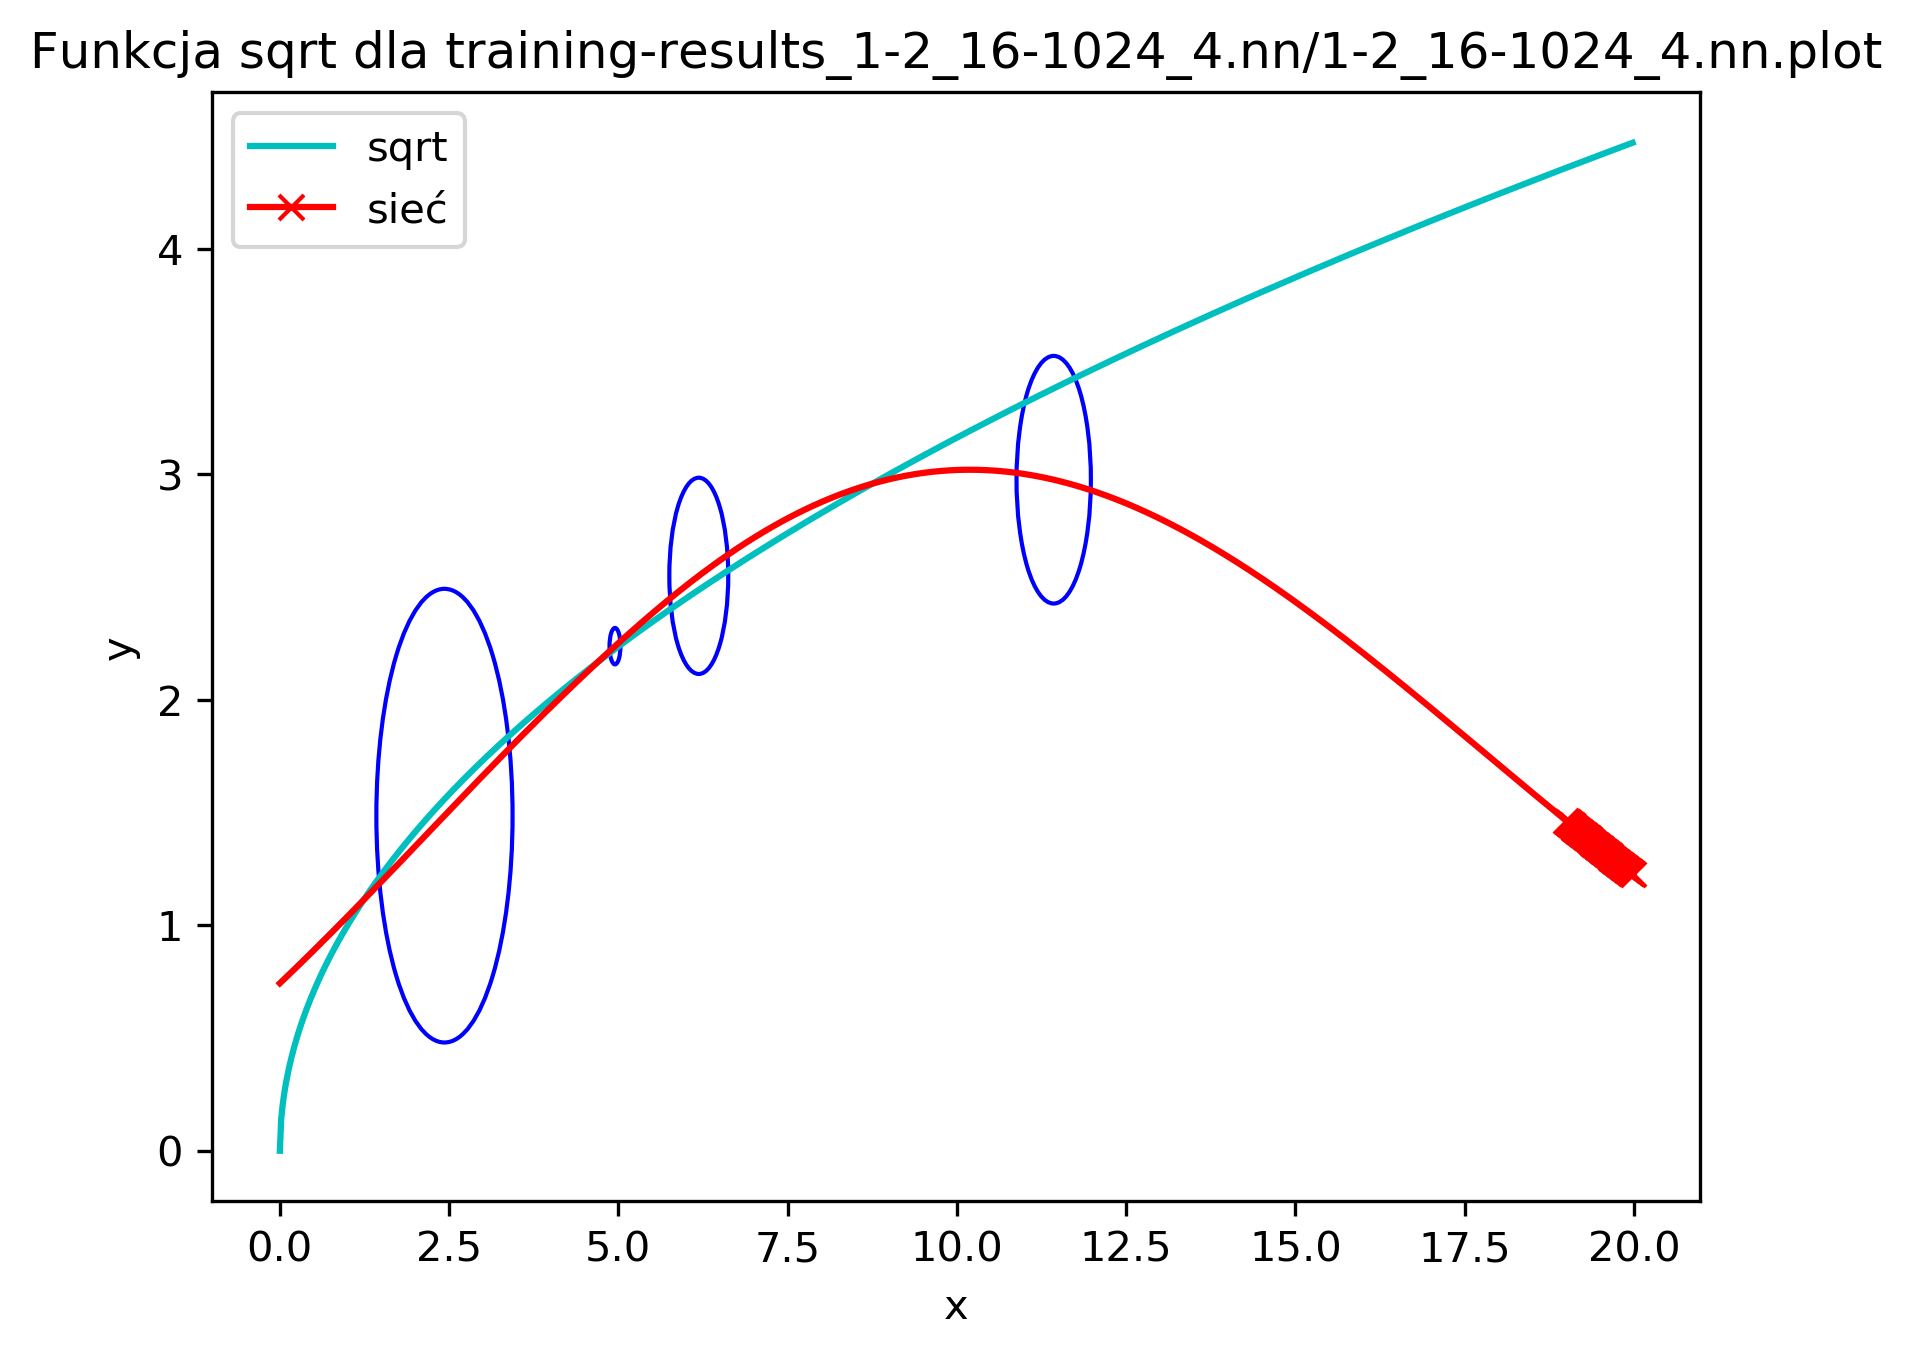
\includegraphics[width=105mm]{wykresy/1-2_16-1024_4_nn_plot.png}
                \end{figure}
                \begin{figure}[!htbp]
                    \centering
                    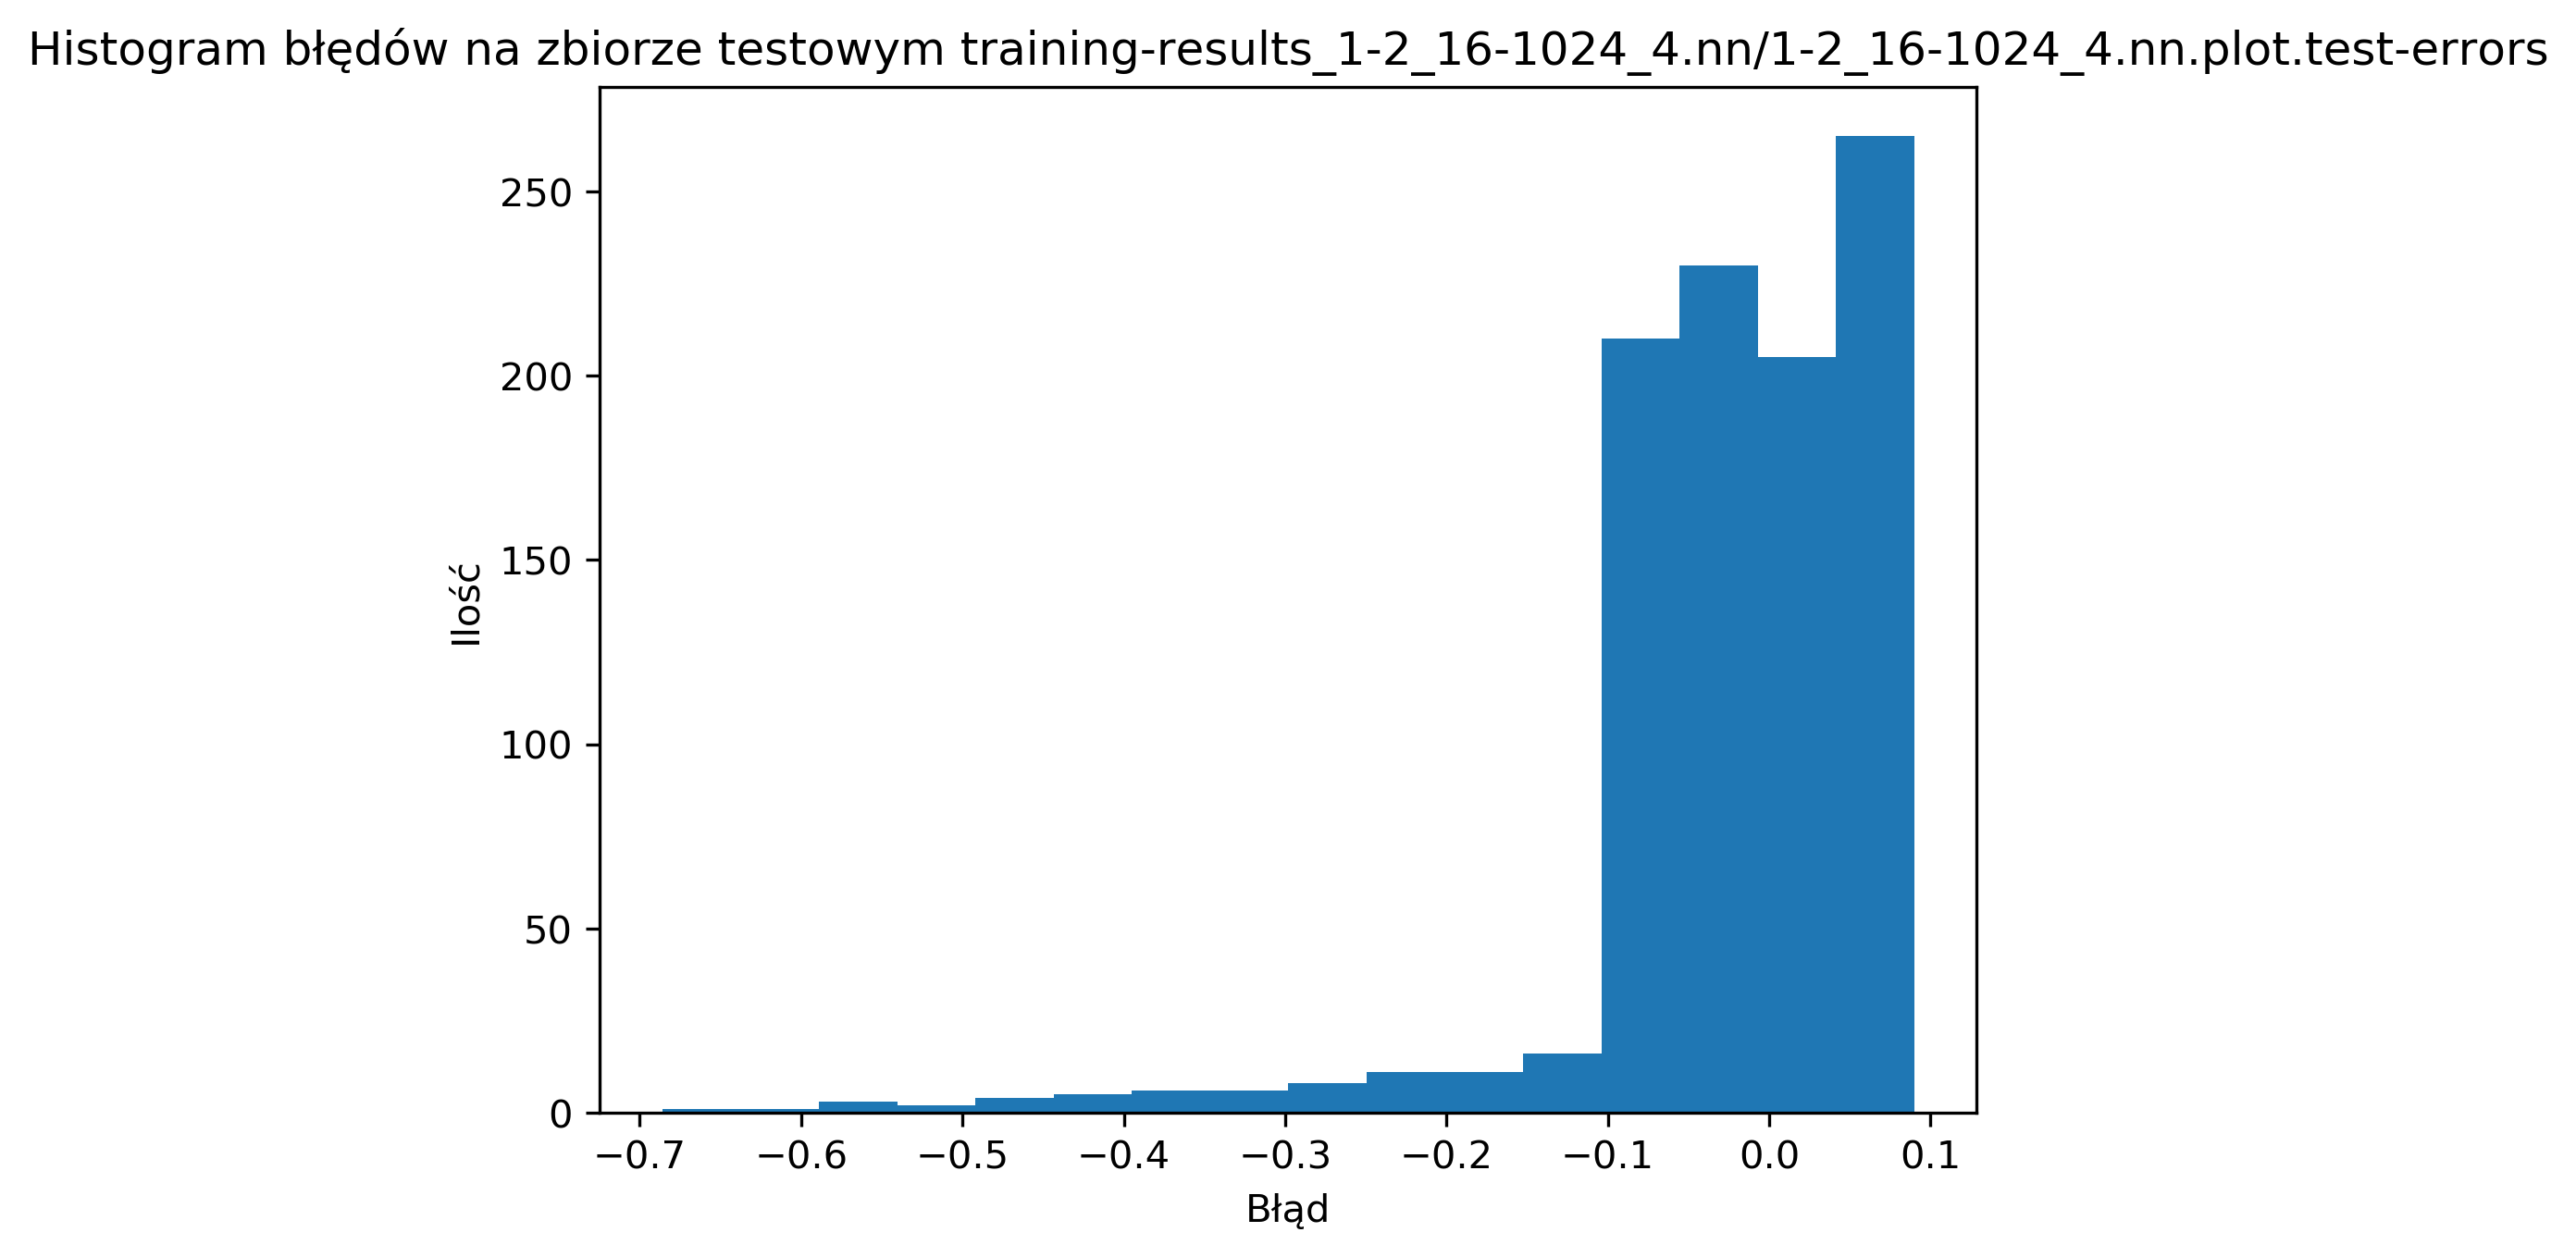
\includegraphics[width=140mm]{wykresy/1-2_16-1024_4_nn_plot_test-errors.png}
                \end{figure}
                \begin{figure}[!htbp]
                    \centering
                    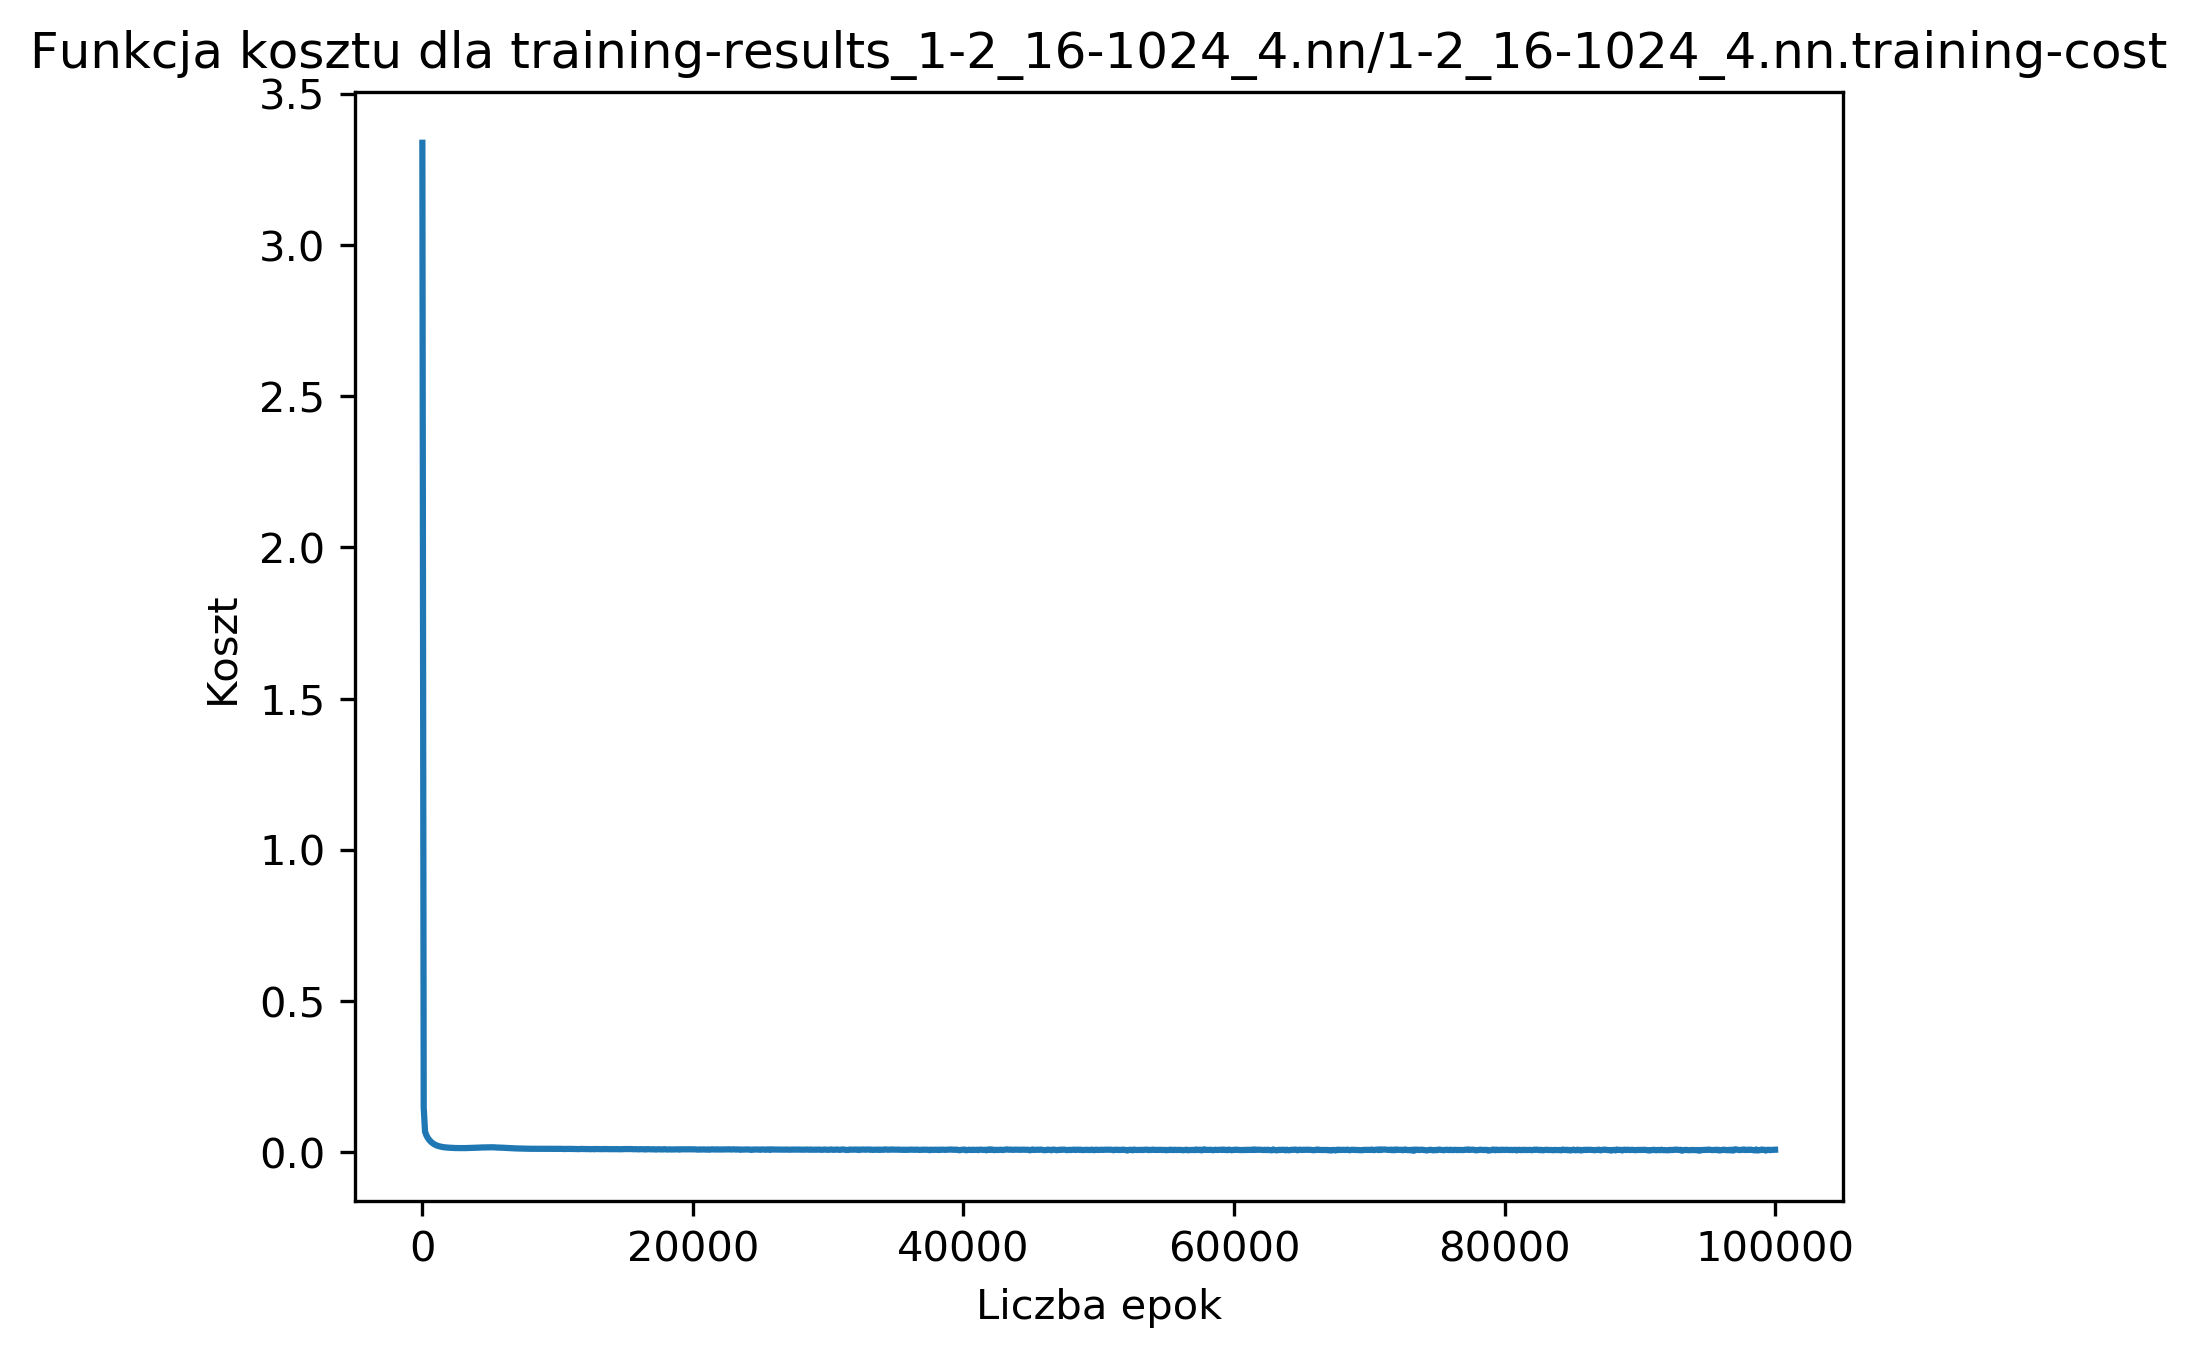
\includegraphics[width=120mm]{wykresy/1-2_16-1024_4_nn_training-cost.png}
                \end{figure}
                \begin{figure}[!htbp]
                    \centering
                    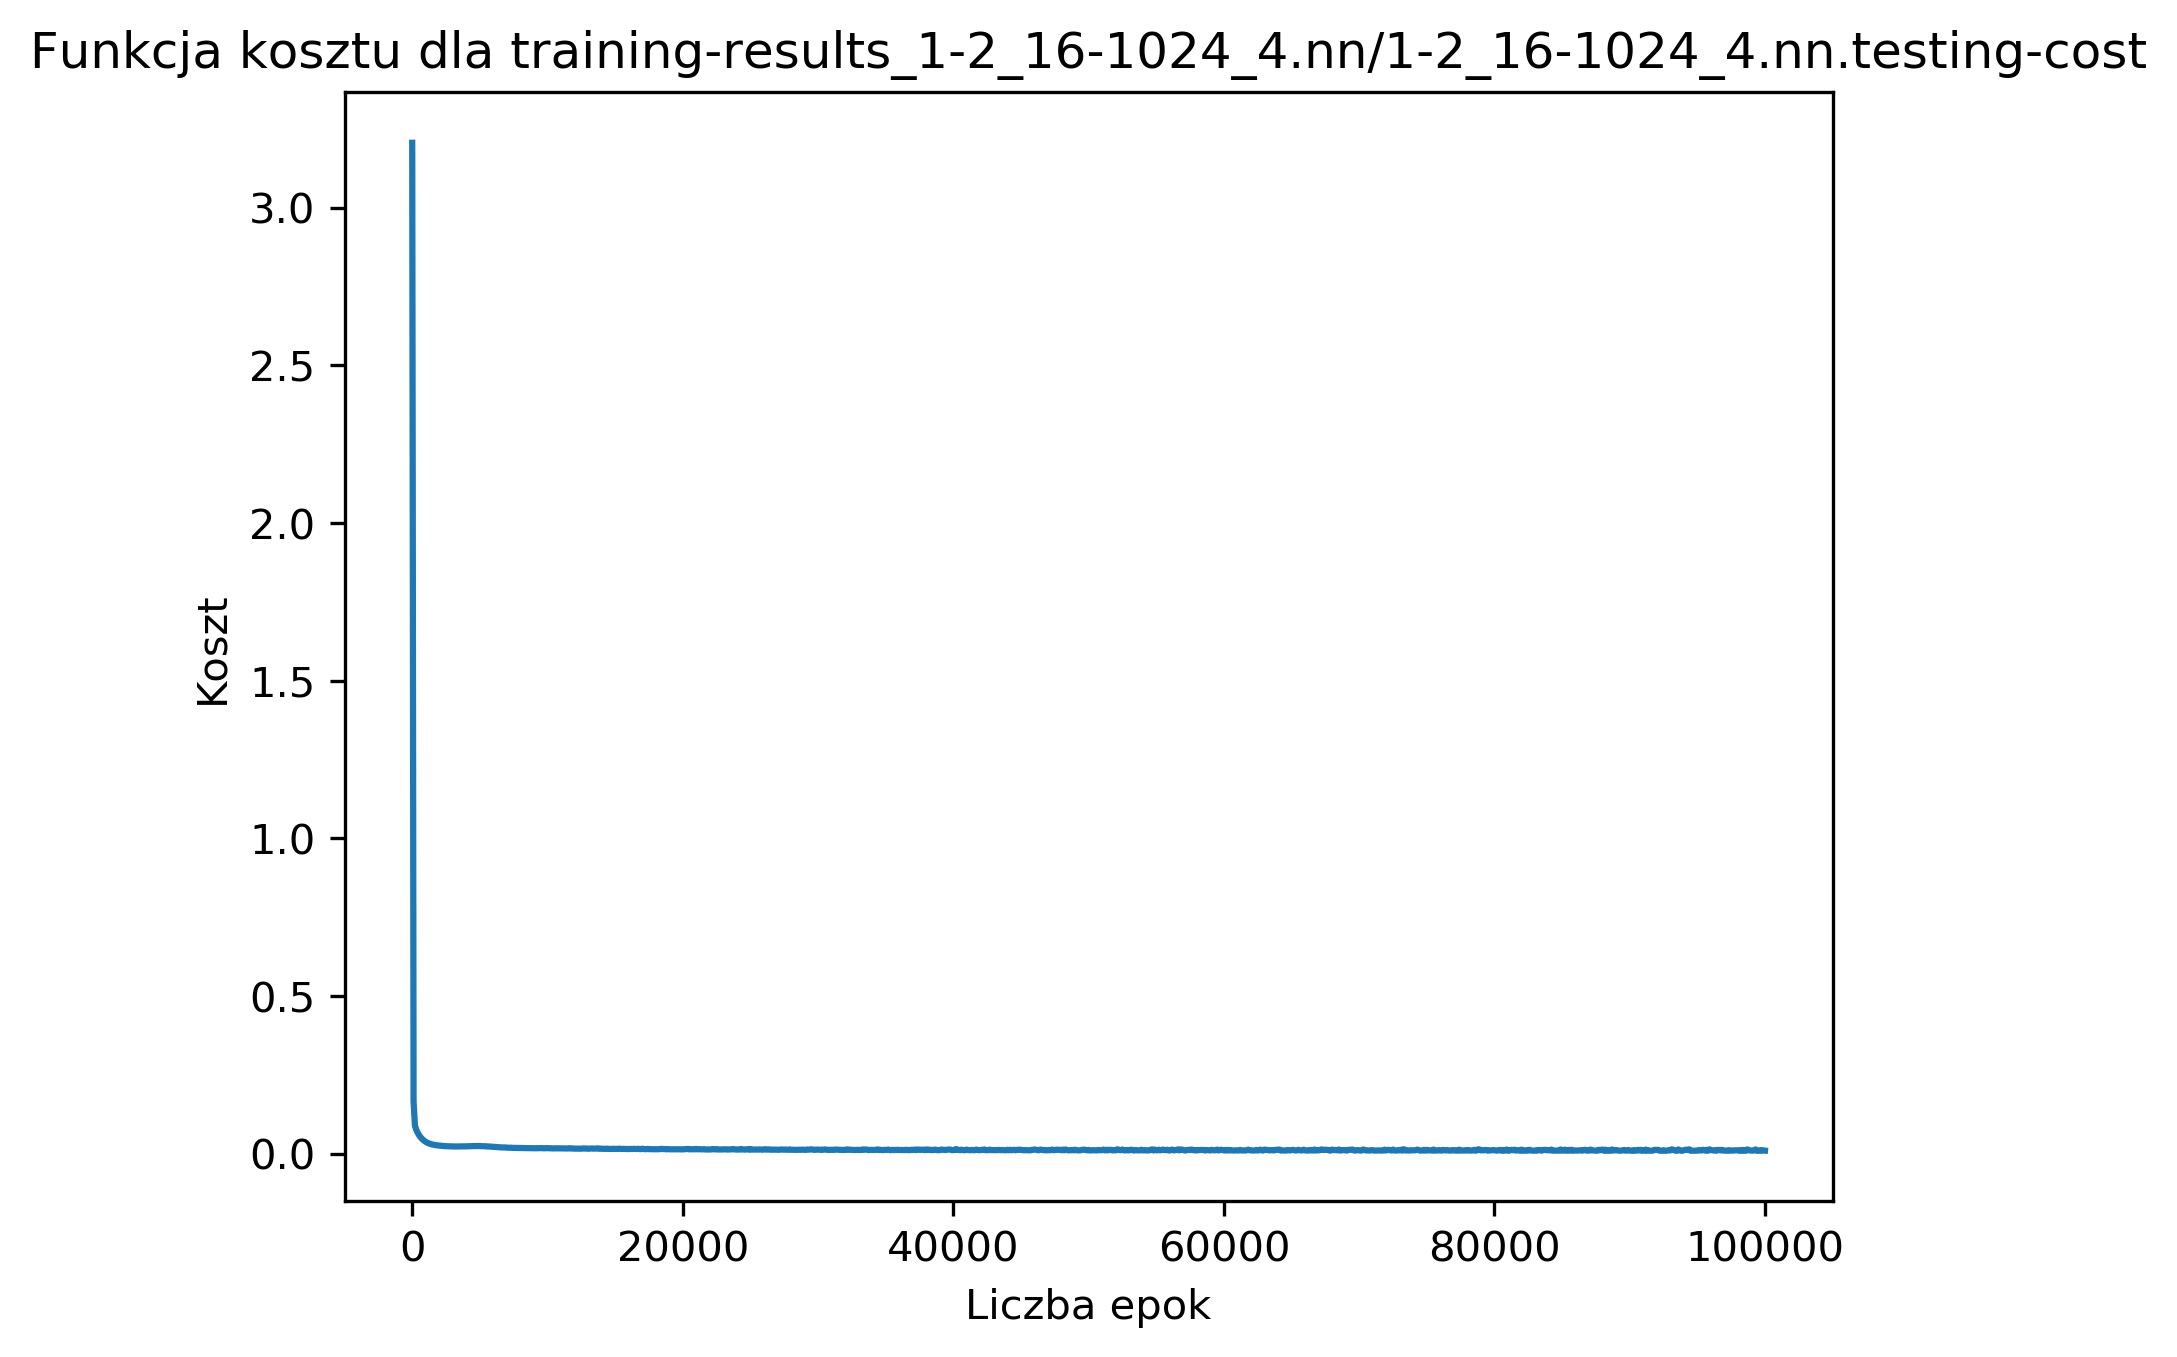
\includegraphics[width=120mm]{wykresy/1-2_16-1024_4_nn_testing-cost.png}
                \end{figure}
                \begin{figure}[!htbp]
                    \centering
                    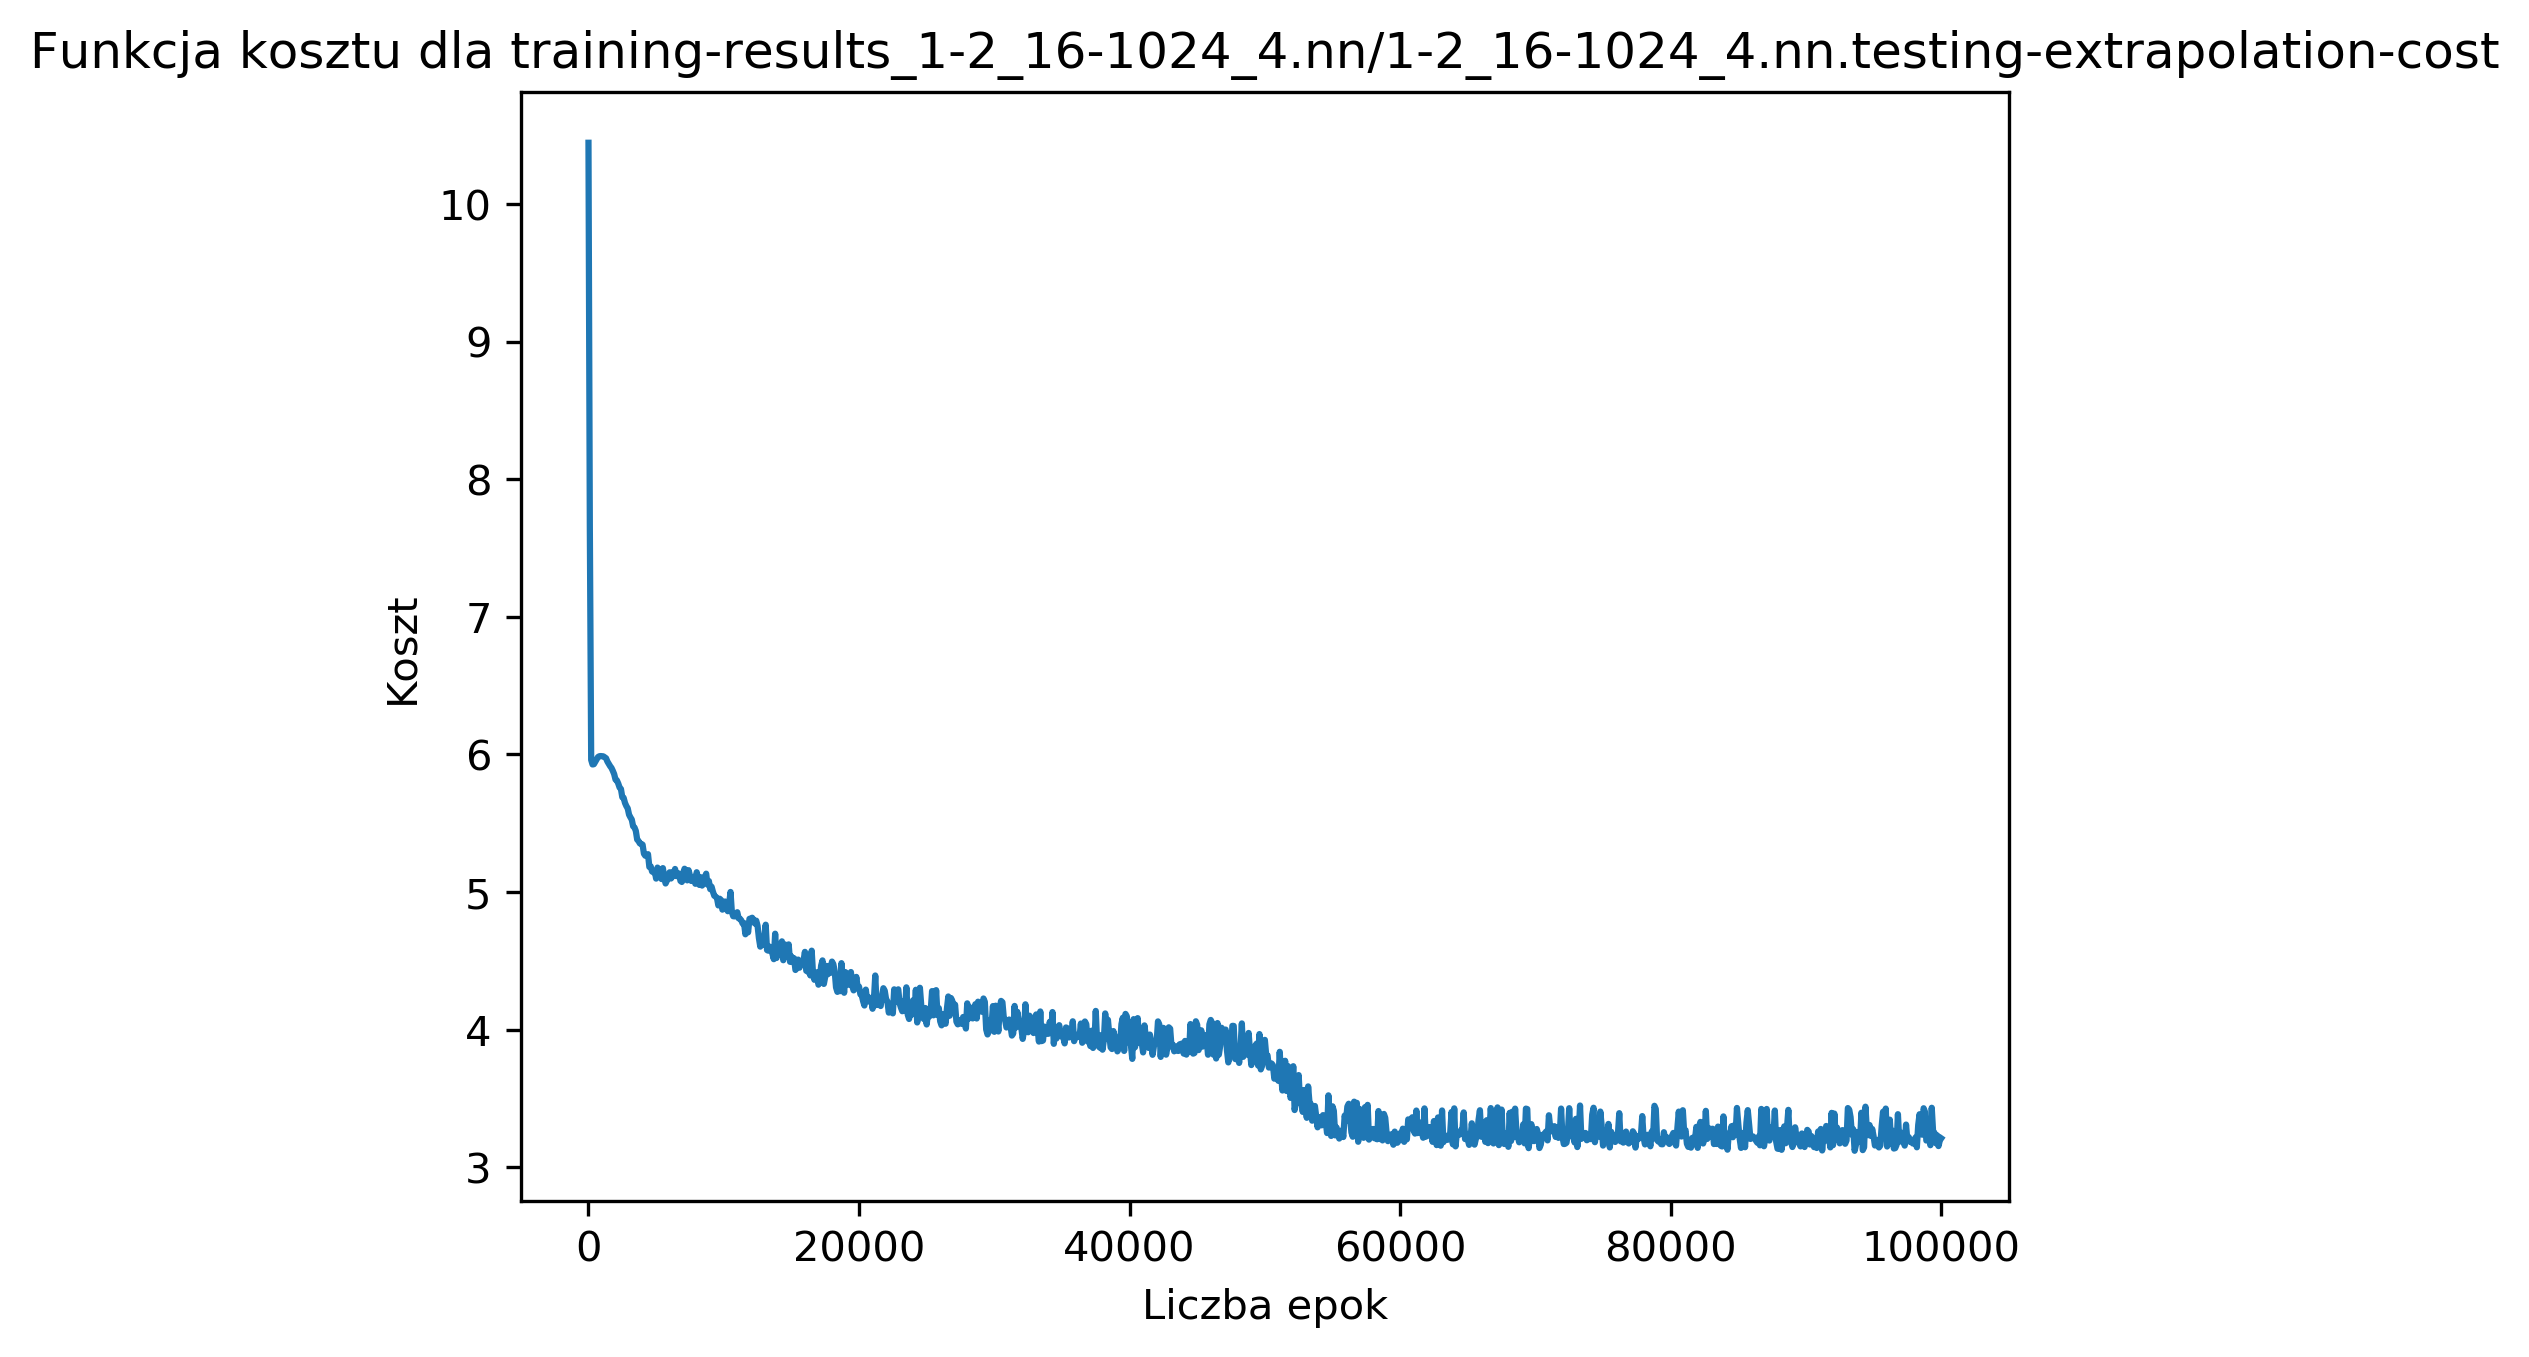
\includegraphics[width=140mm]{wykresy/1-2_16-1024_4_nn_testing-extrapolation-cost.png}
                \end{figure}
                \FloatBarrier
            %---------------------------------------------------%
                \begin{figure}[!htbp]
                    \centering
                    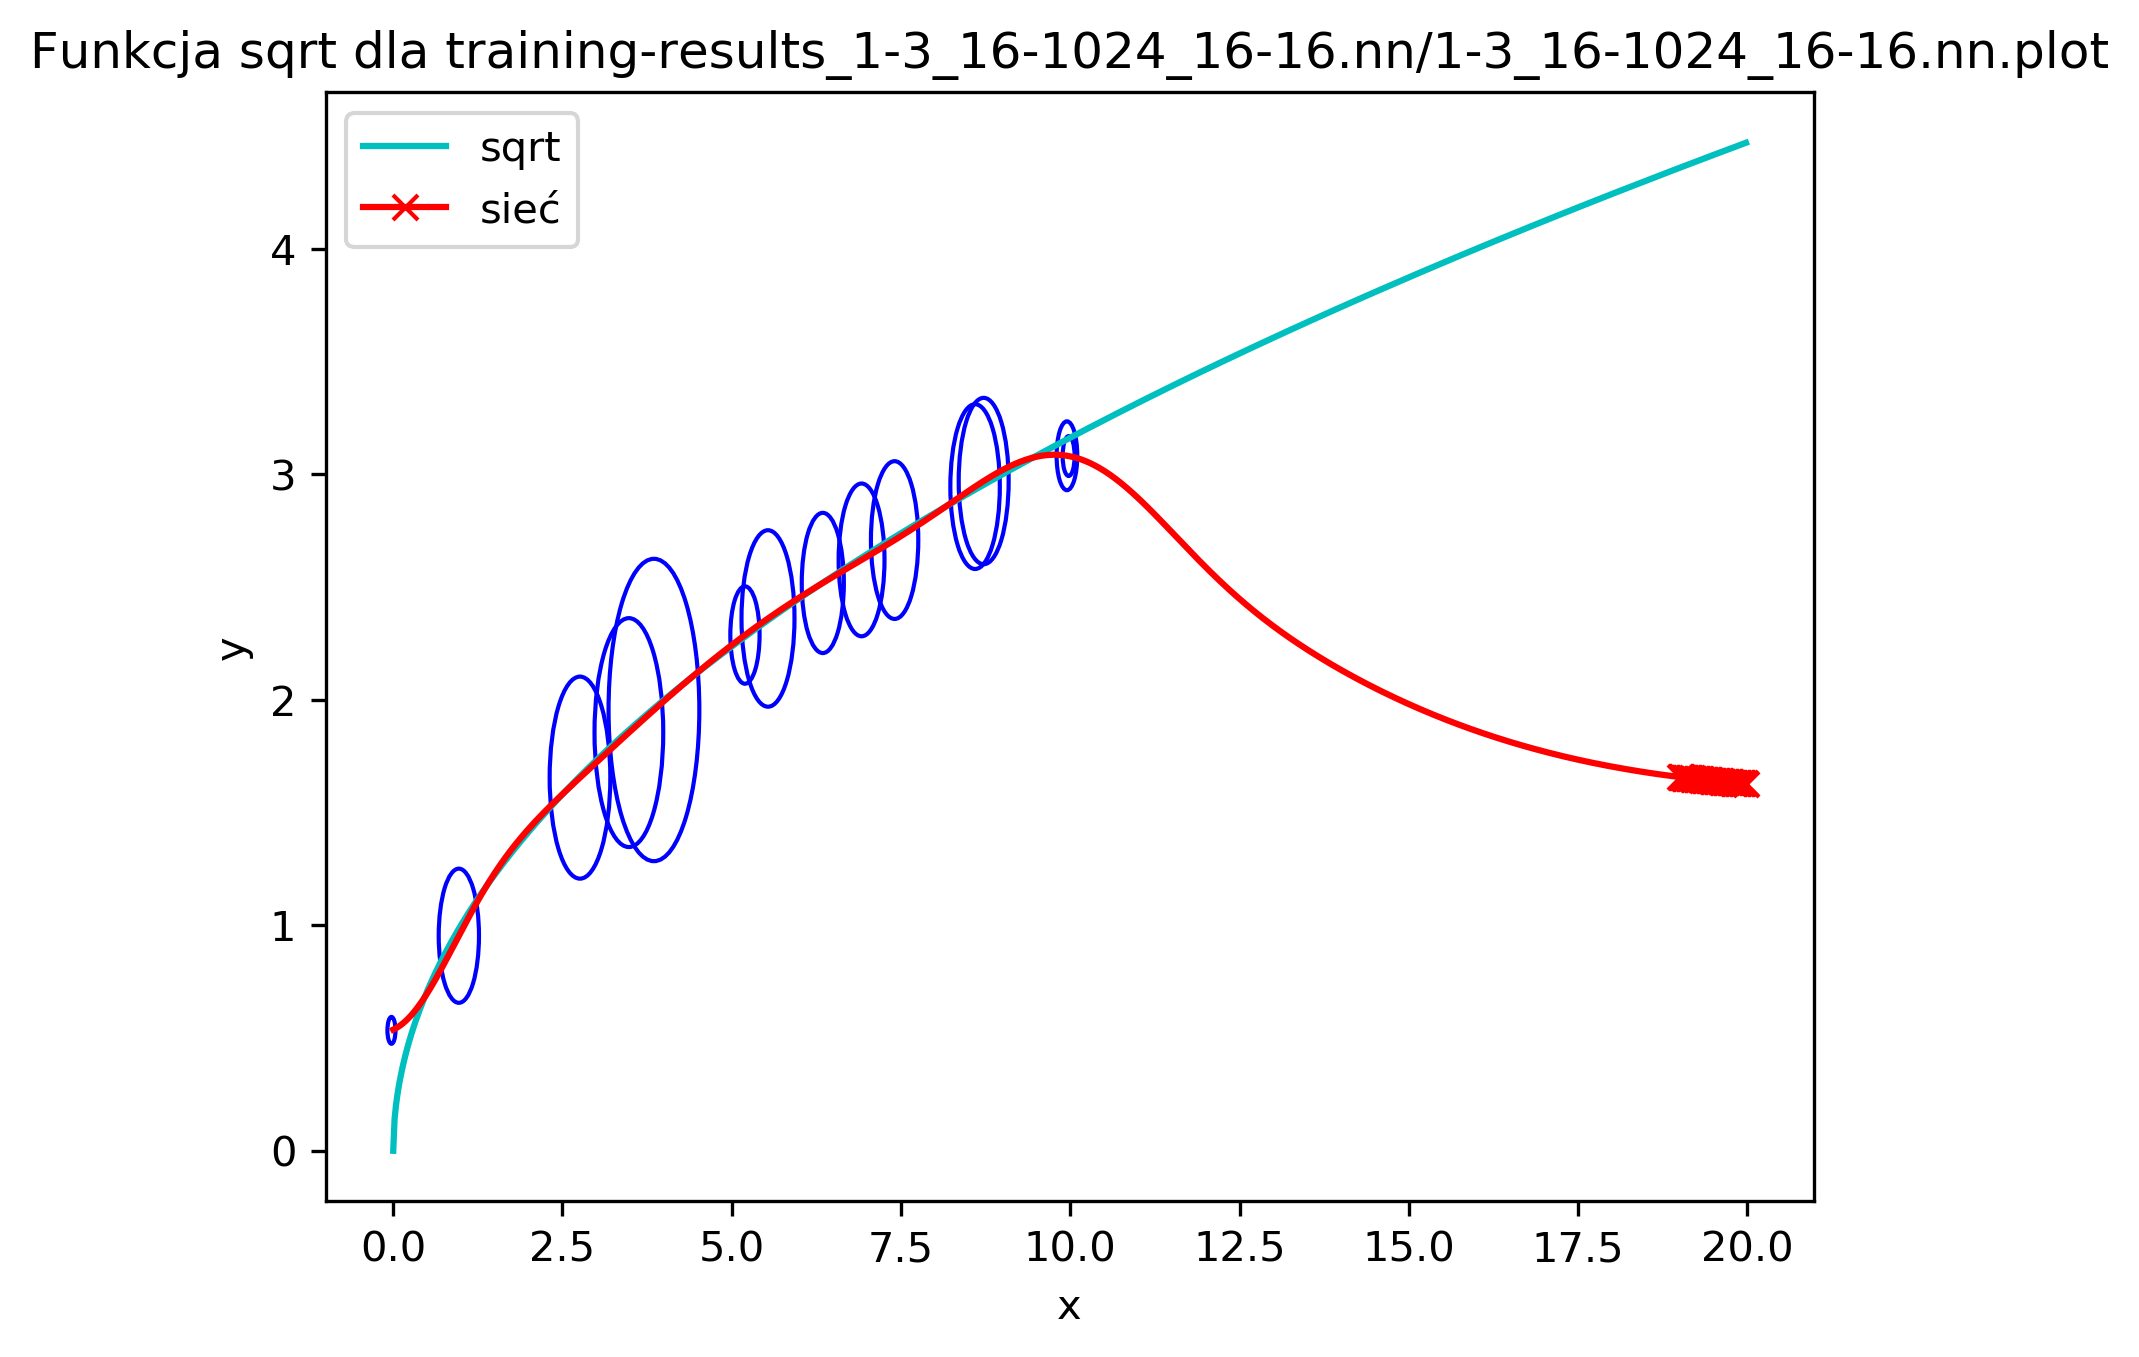
\includegraphics[width=105mm]{wykresy/1-3_16-1024_16-16_nn_plot.png}
                \end{figure}
                \begin{figure}[!htbp]
                    \centering
                    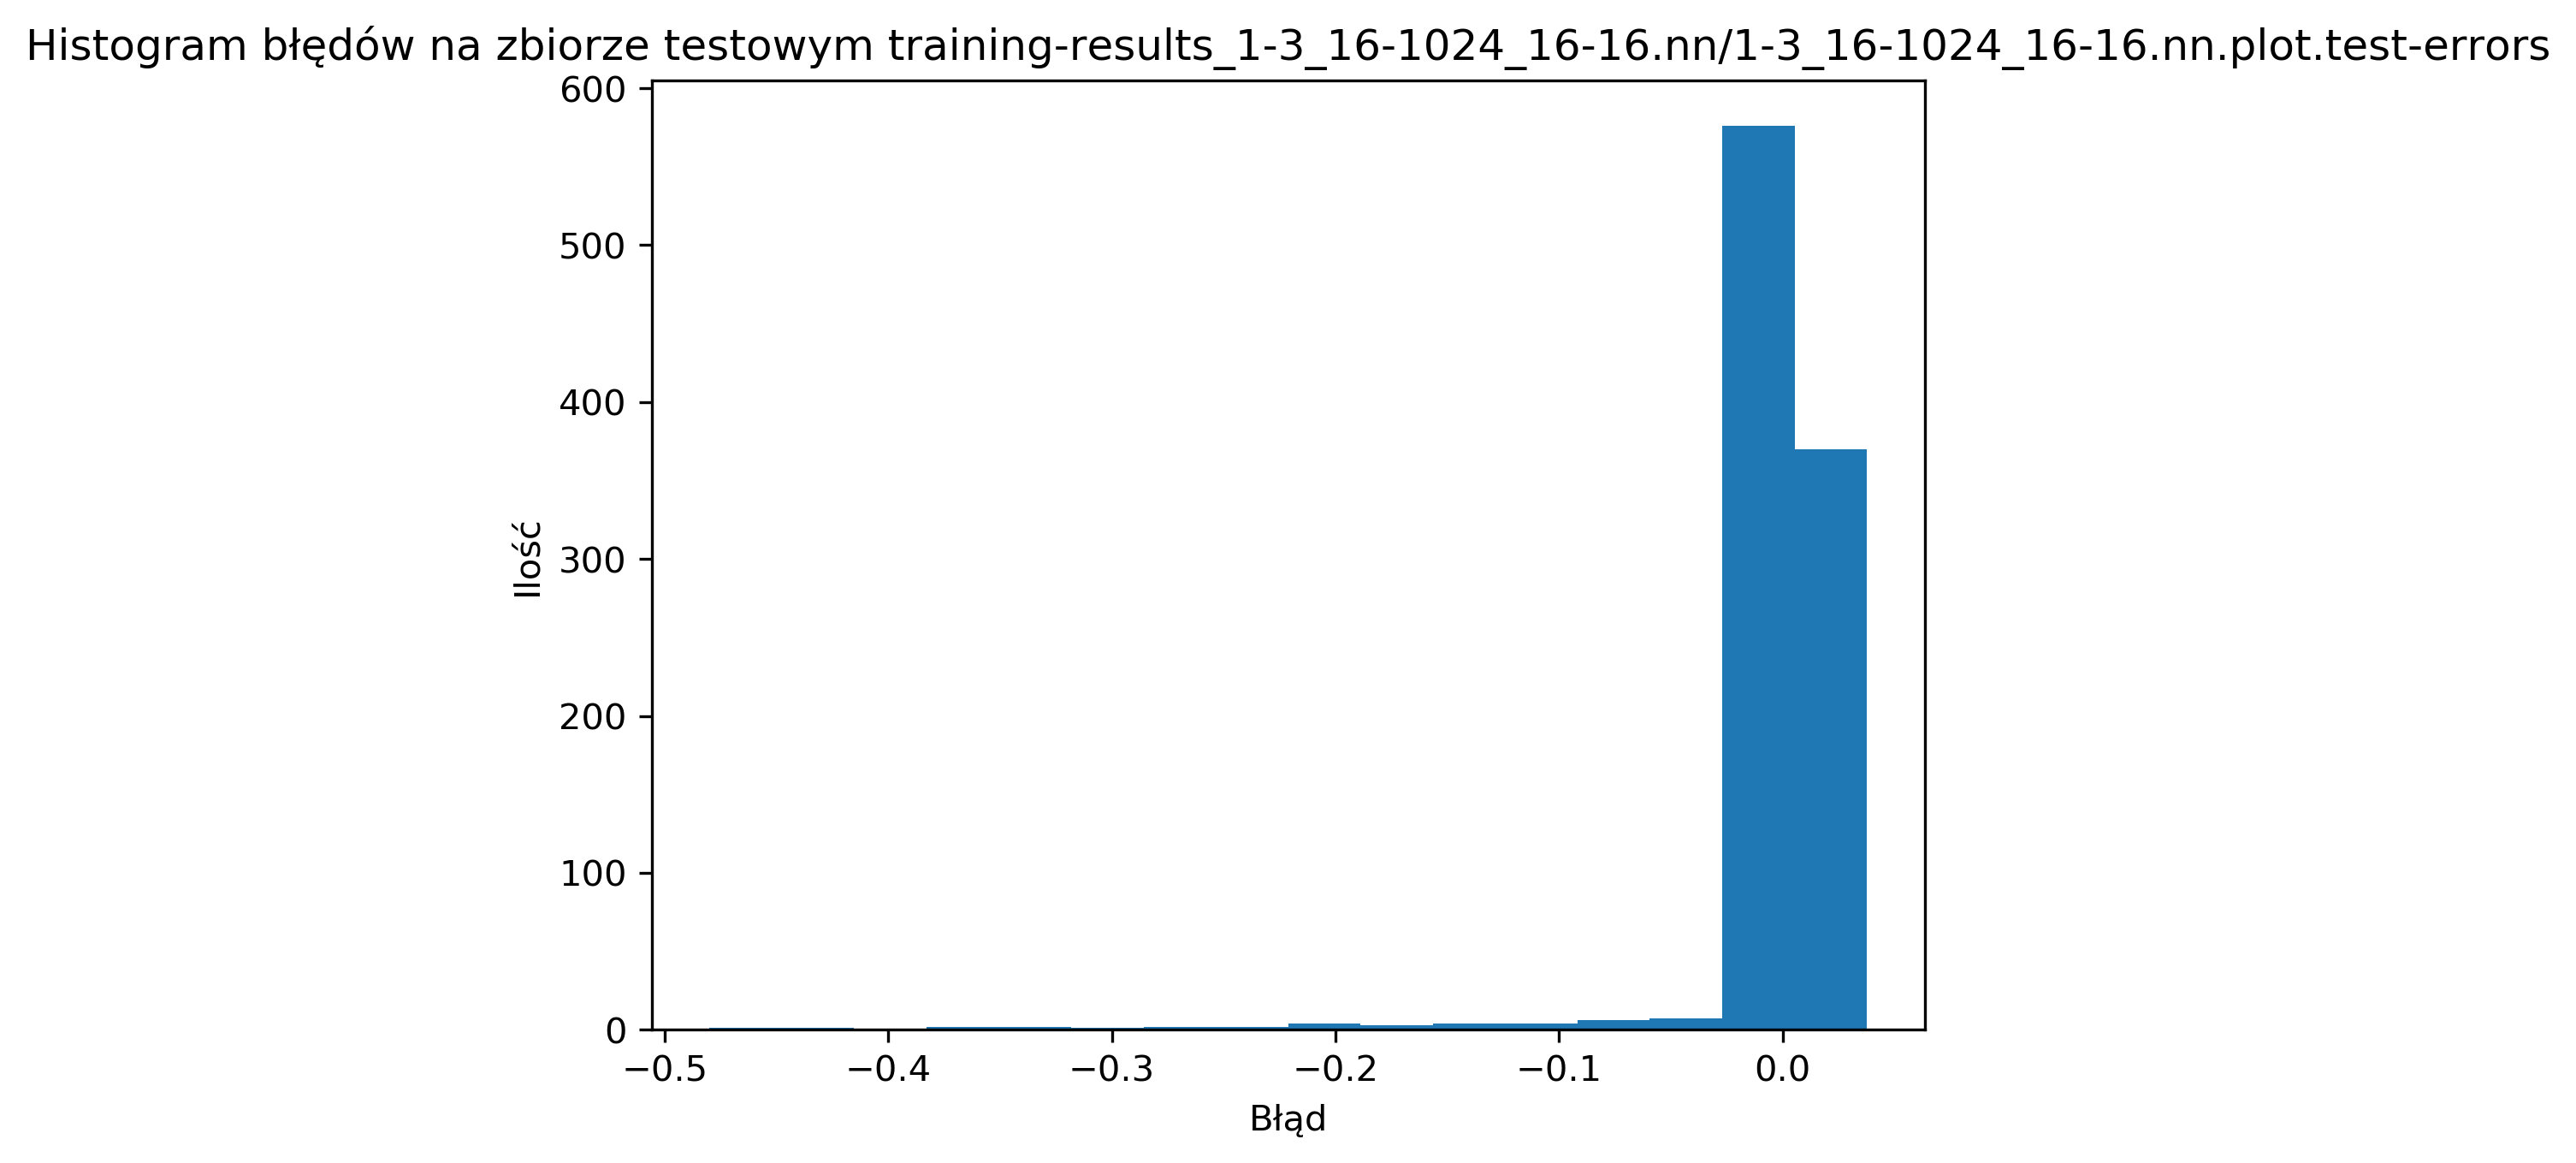
\includegraphics[width=140mm]{wykresy/1-3_16-1024_16-16_nn_plot_test-errors.png}
                \end{figure}
                \begin{figure}[!htbp]
                    \centering
                    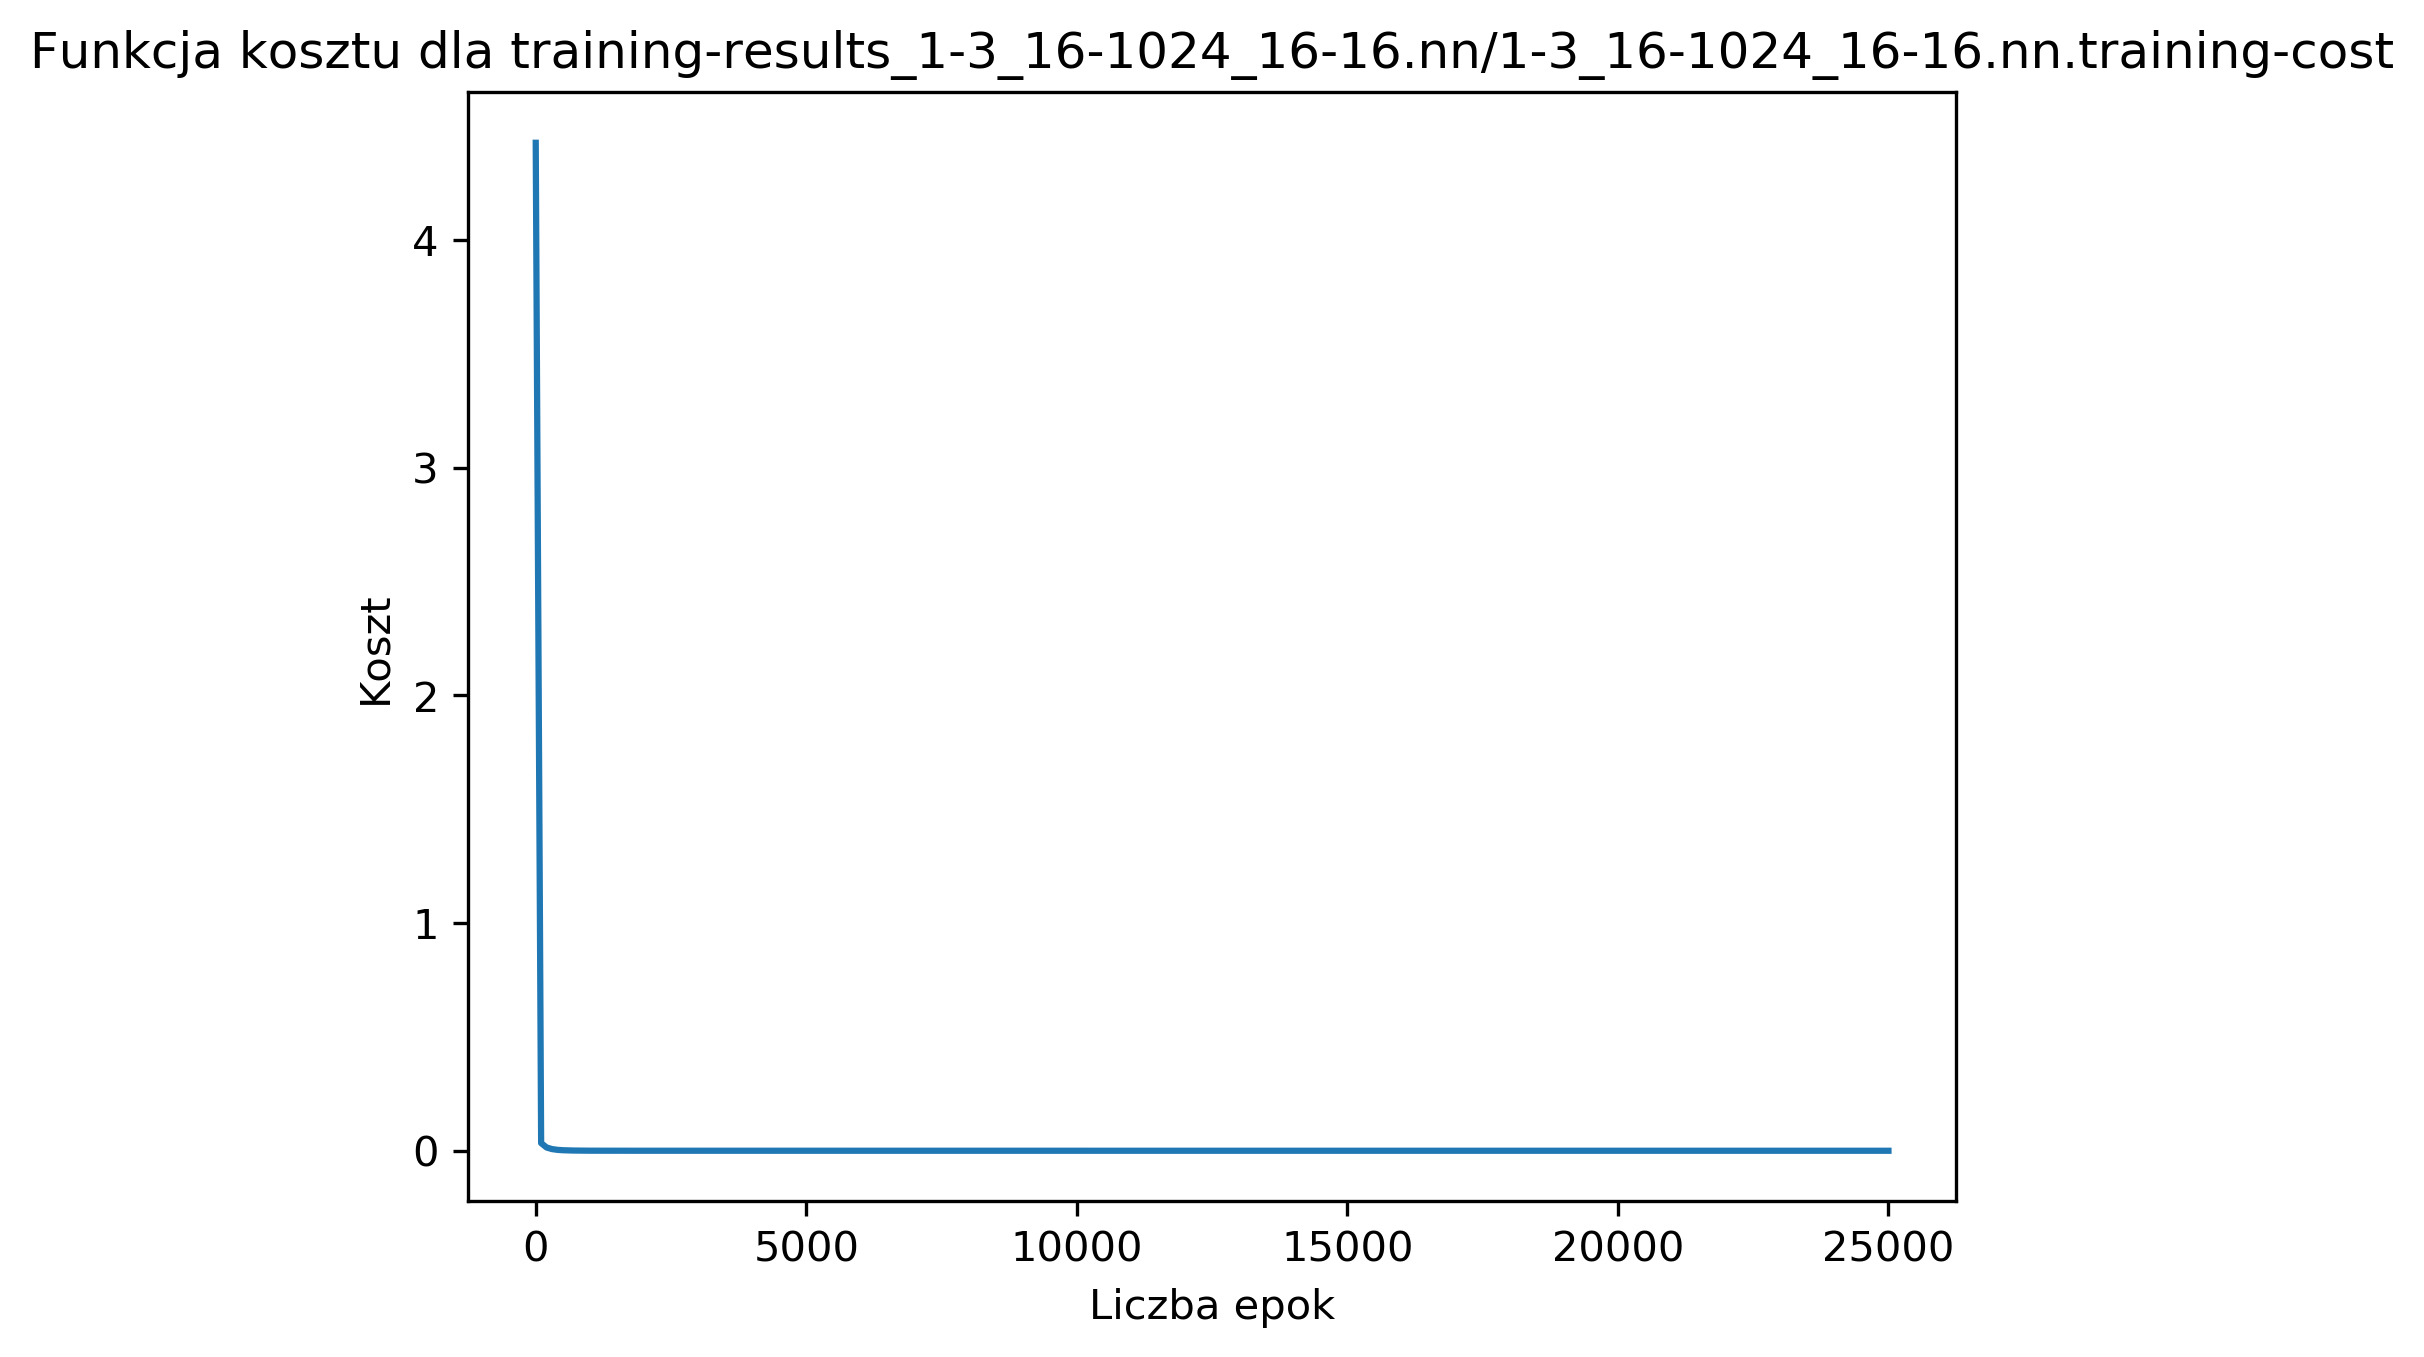
\includegraphics[width=120mm]{wykresy/1-3_16-1024_16-16_nn_training-cost.png}
                \end{figure}
                \begin{figure}[!htbp]
                    \centering
                    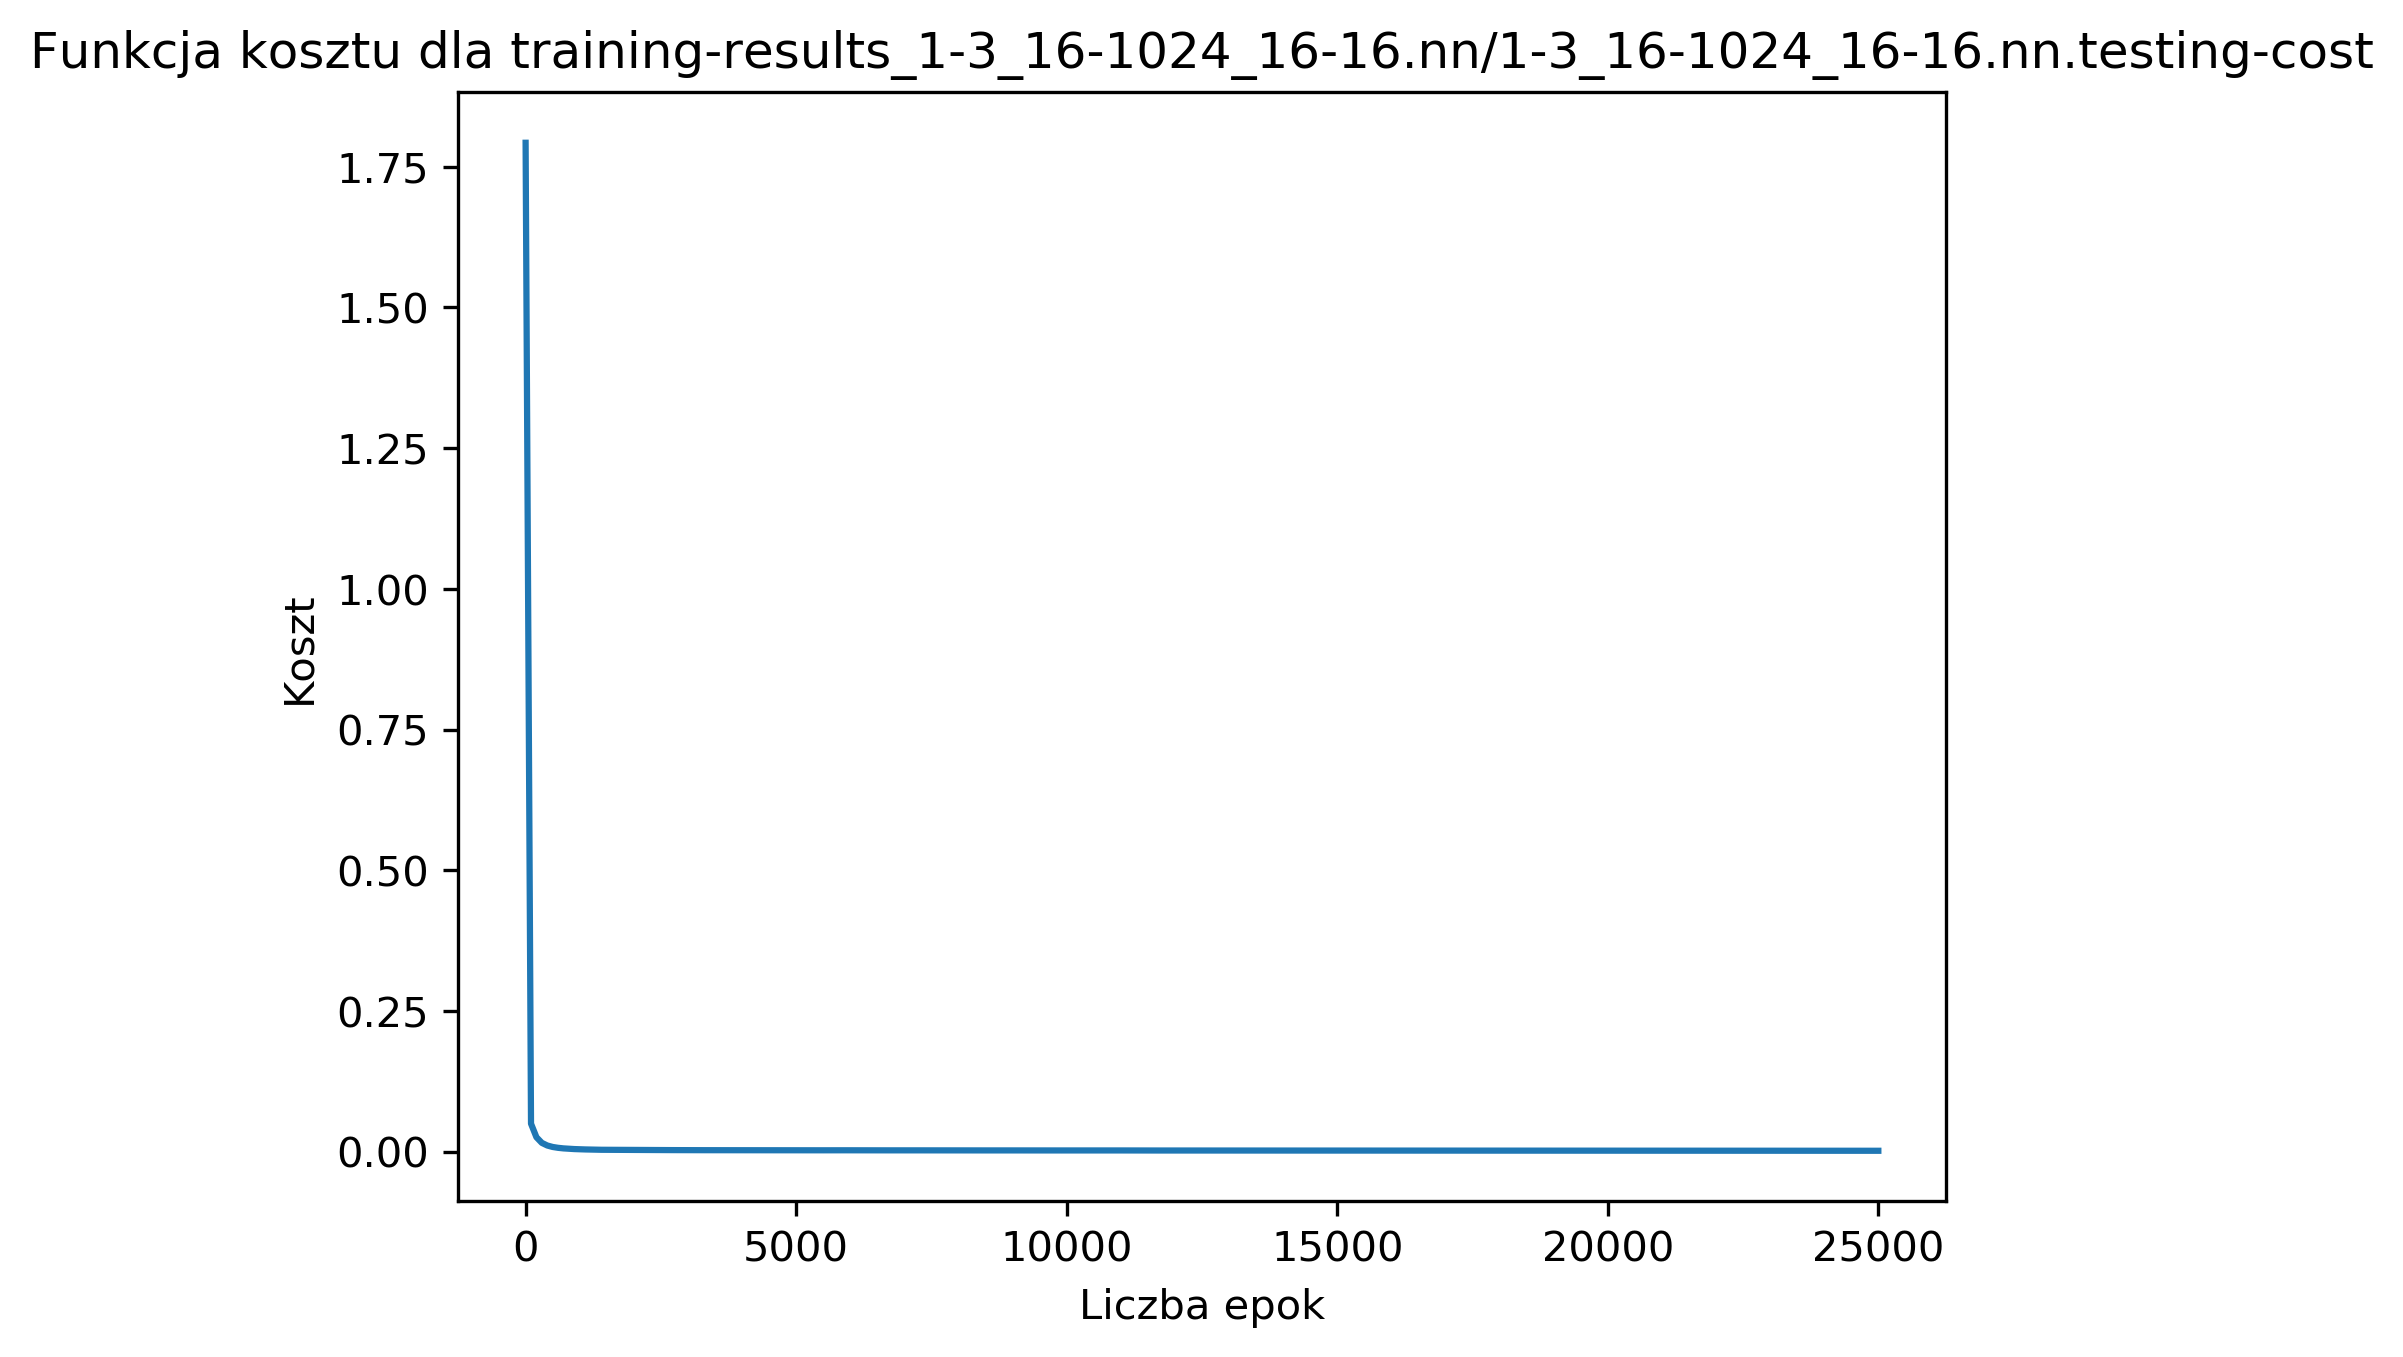
\includegraphics[width=120mm]{wykresy/1-3_16-1024_16-16_nn_testing-cost.png}
                \end{figure}
                \begin{figure}[!htbp]
                    \centering
                    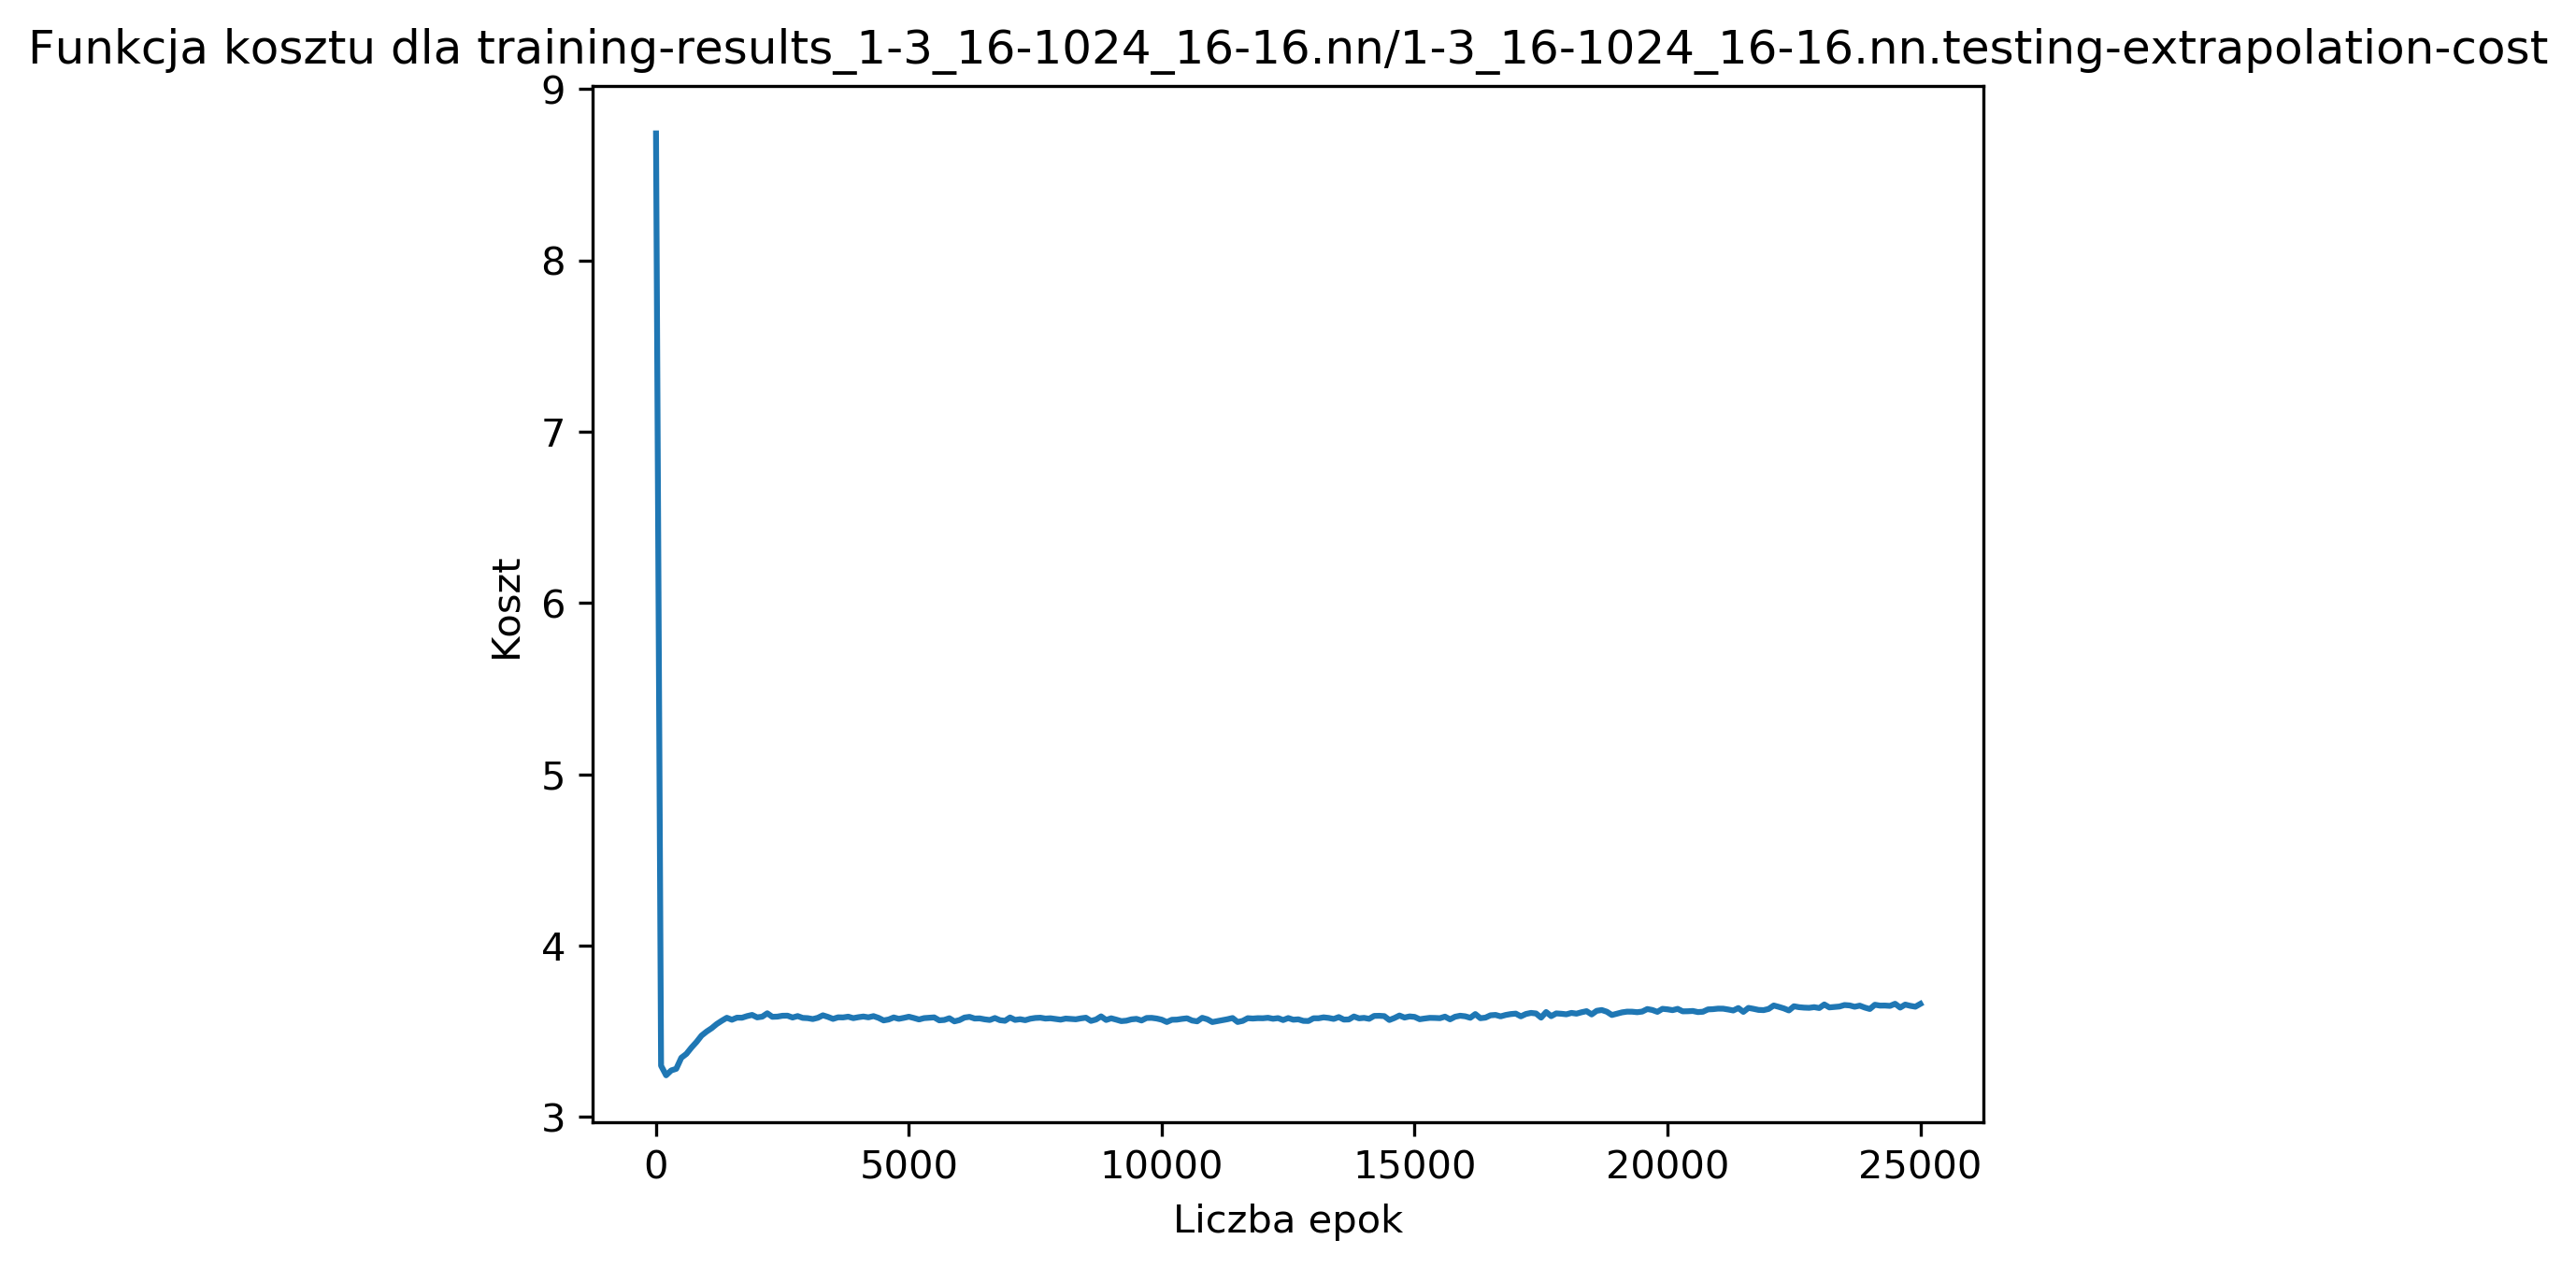
\includegraphics[width=140mm]{wykresy/1-3_16-1024_16-16_nn_testing-extrapolation-cost.png}
                \end{figure}
                \FloatBarrier
            %---------------------------------------------------%
            }

            \subsubsection{Badanie liczby punktów treningowych}
            {
                \begin{figure}[!htbp]
                    \centering
                    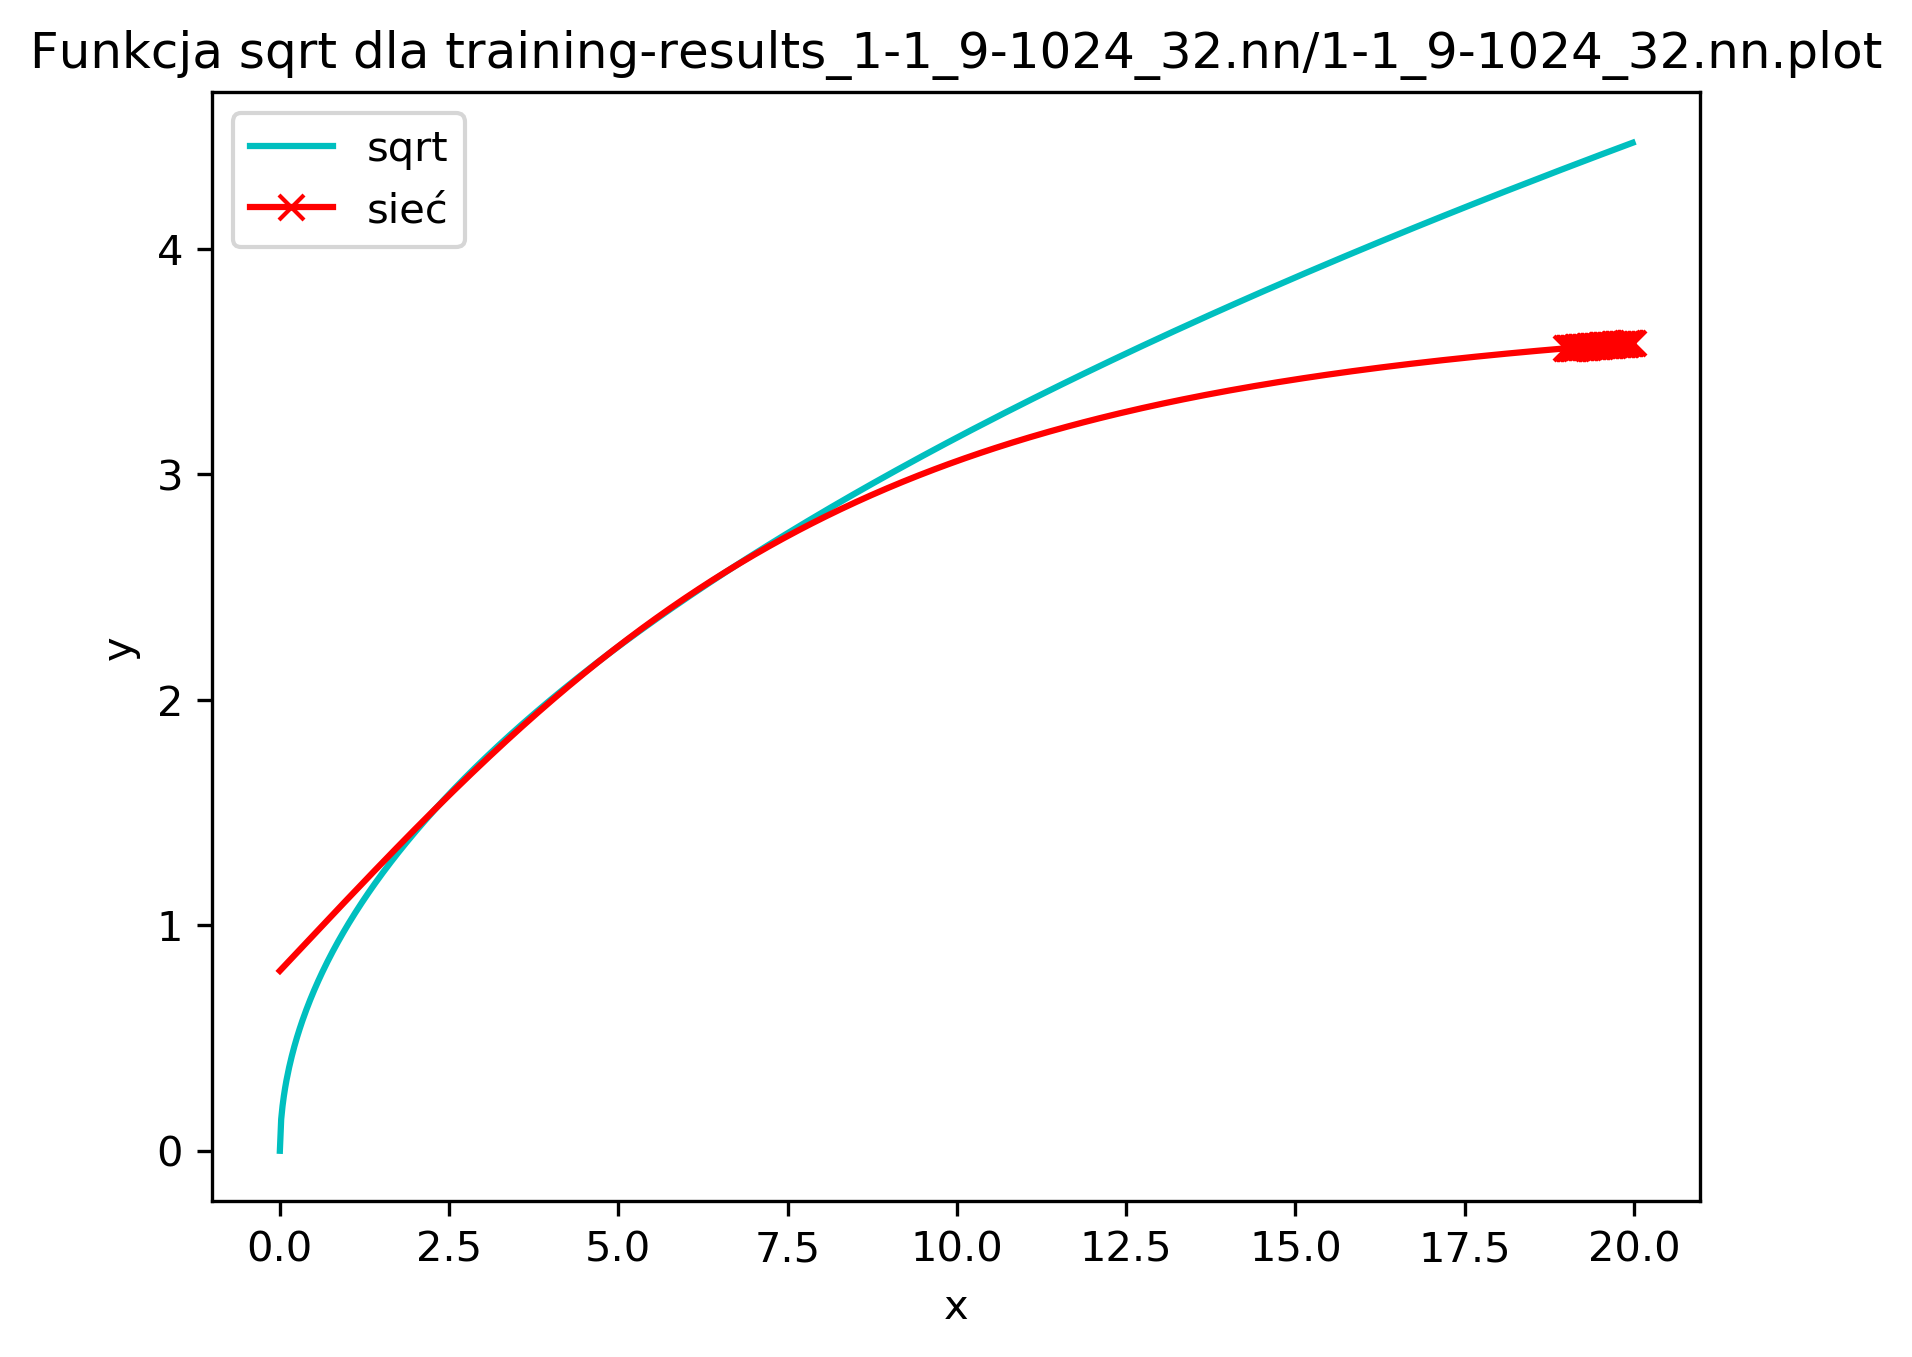
\includegraphics[width=105mm]{wykresy/1-1_9-1024_32_nn_plot.png}
                \end{figure}
                \begin{figure}[!htbp]
                    \centering
                    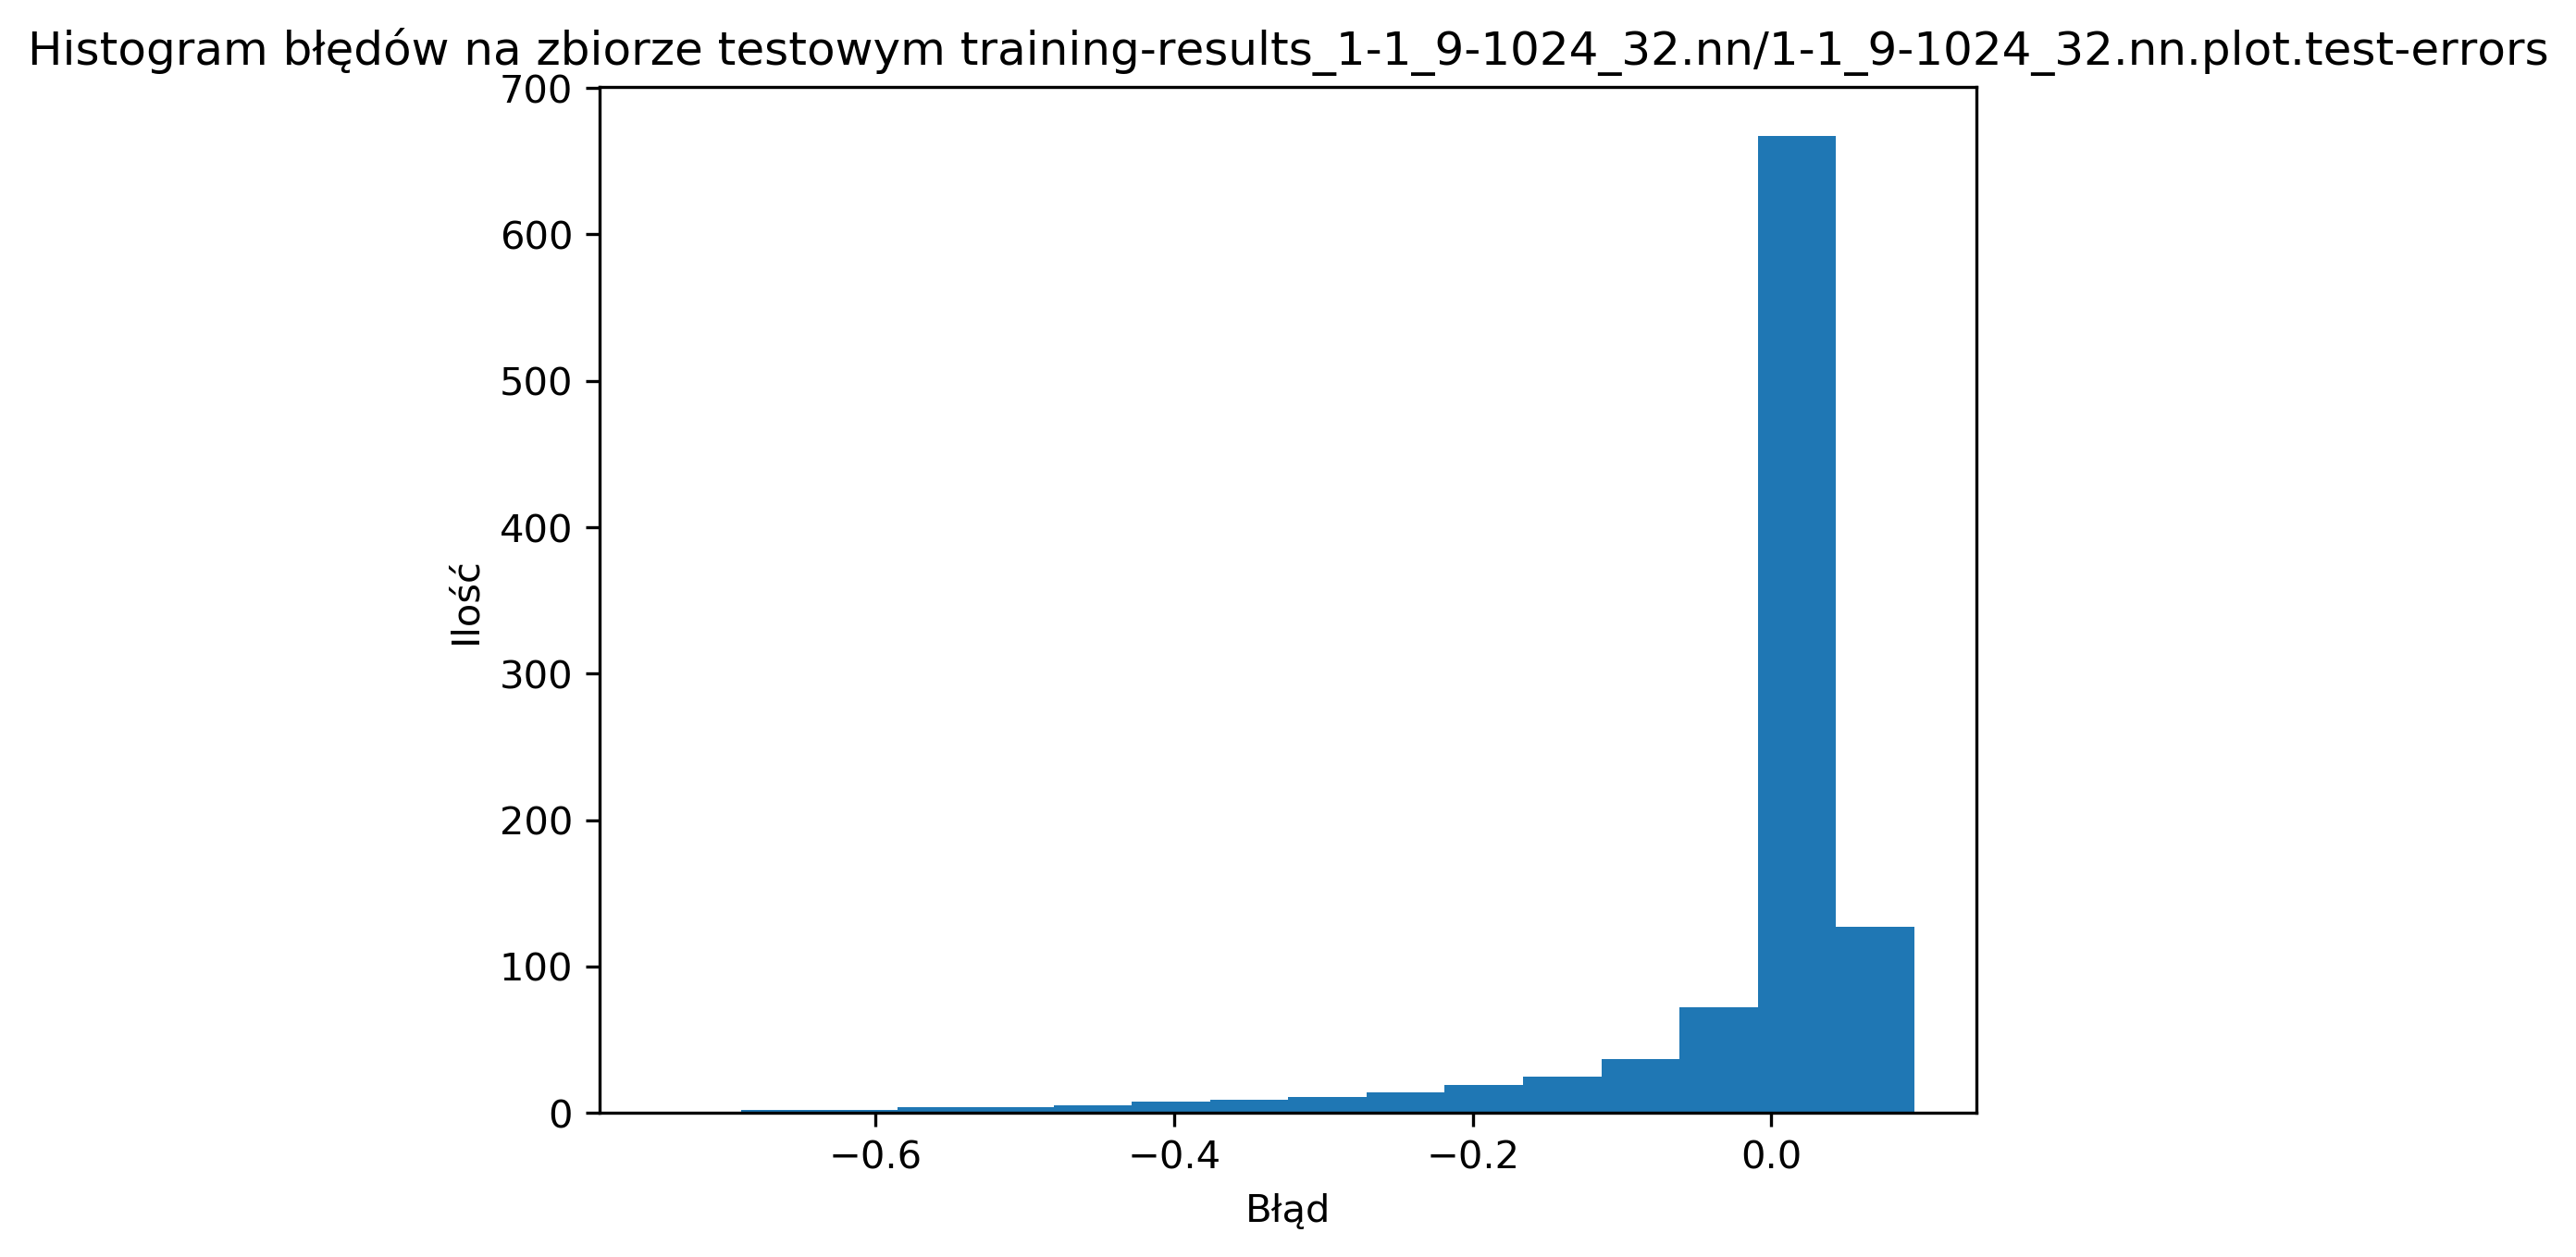
\includegraphics[width=140mm]{wykresy/1-1_9-1024_32_nn_plot_test-errors.png}
                \end{figure}
                \begin{figure}[!htbp]
                    \centering
                    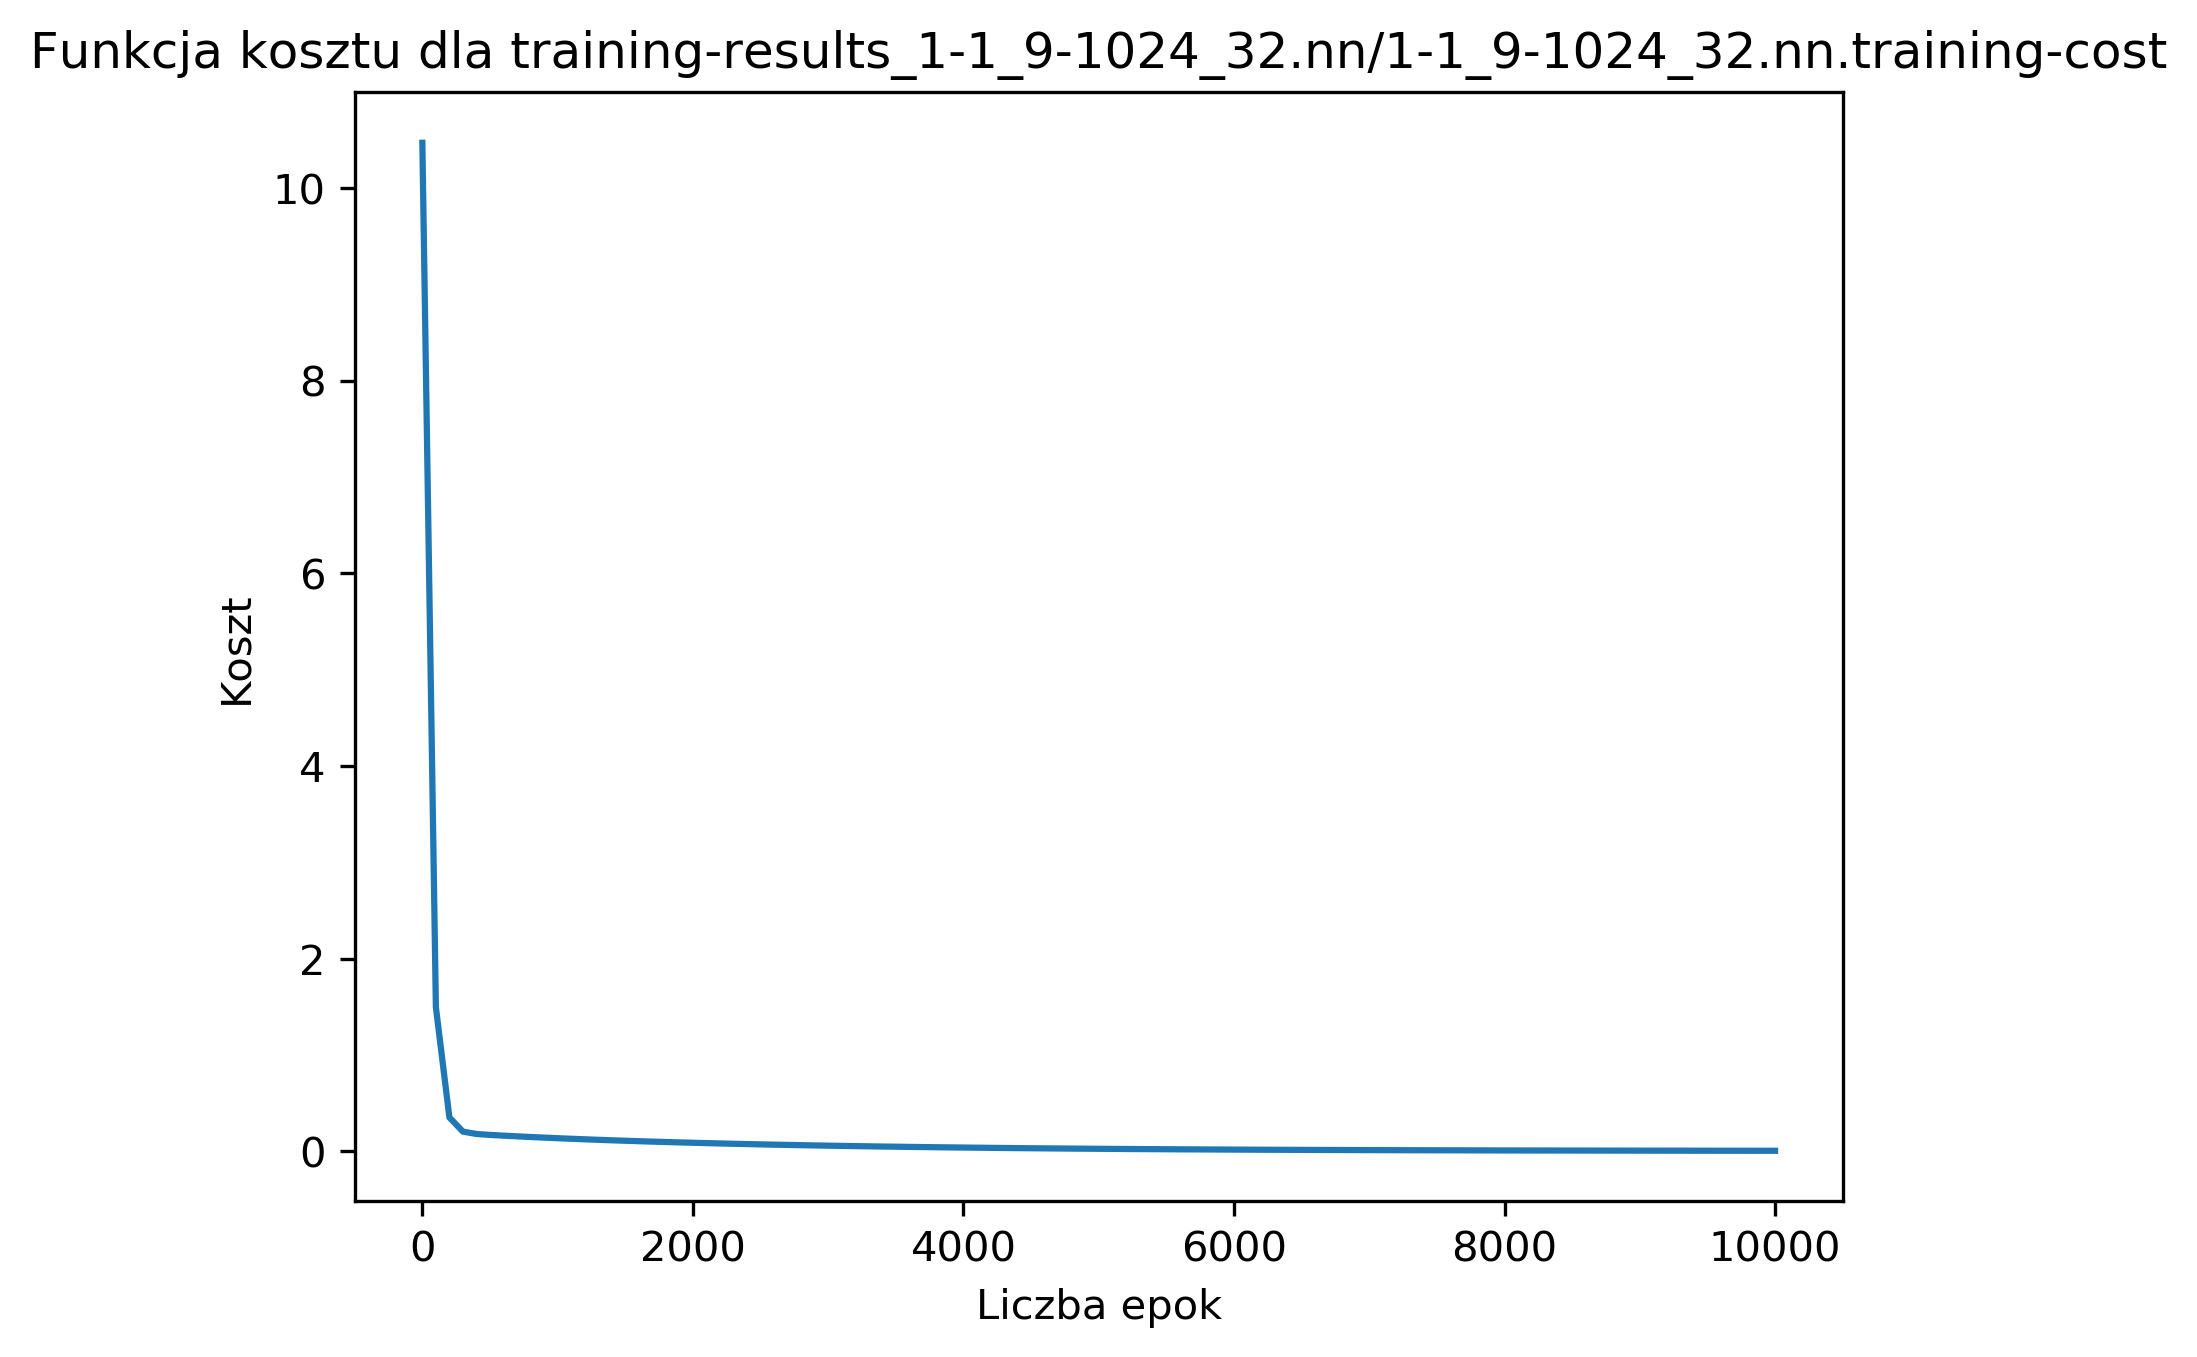
\includegraphics[width=120mm]{wykresy/1-1_9-1024_32_nn_training-cost.png}
                \end{figure}
                \begin{figure}[!htbp]
                    \centering
                    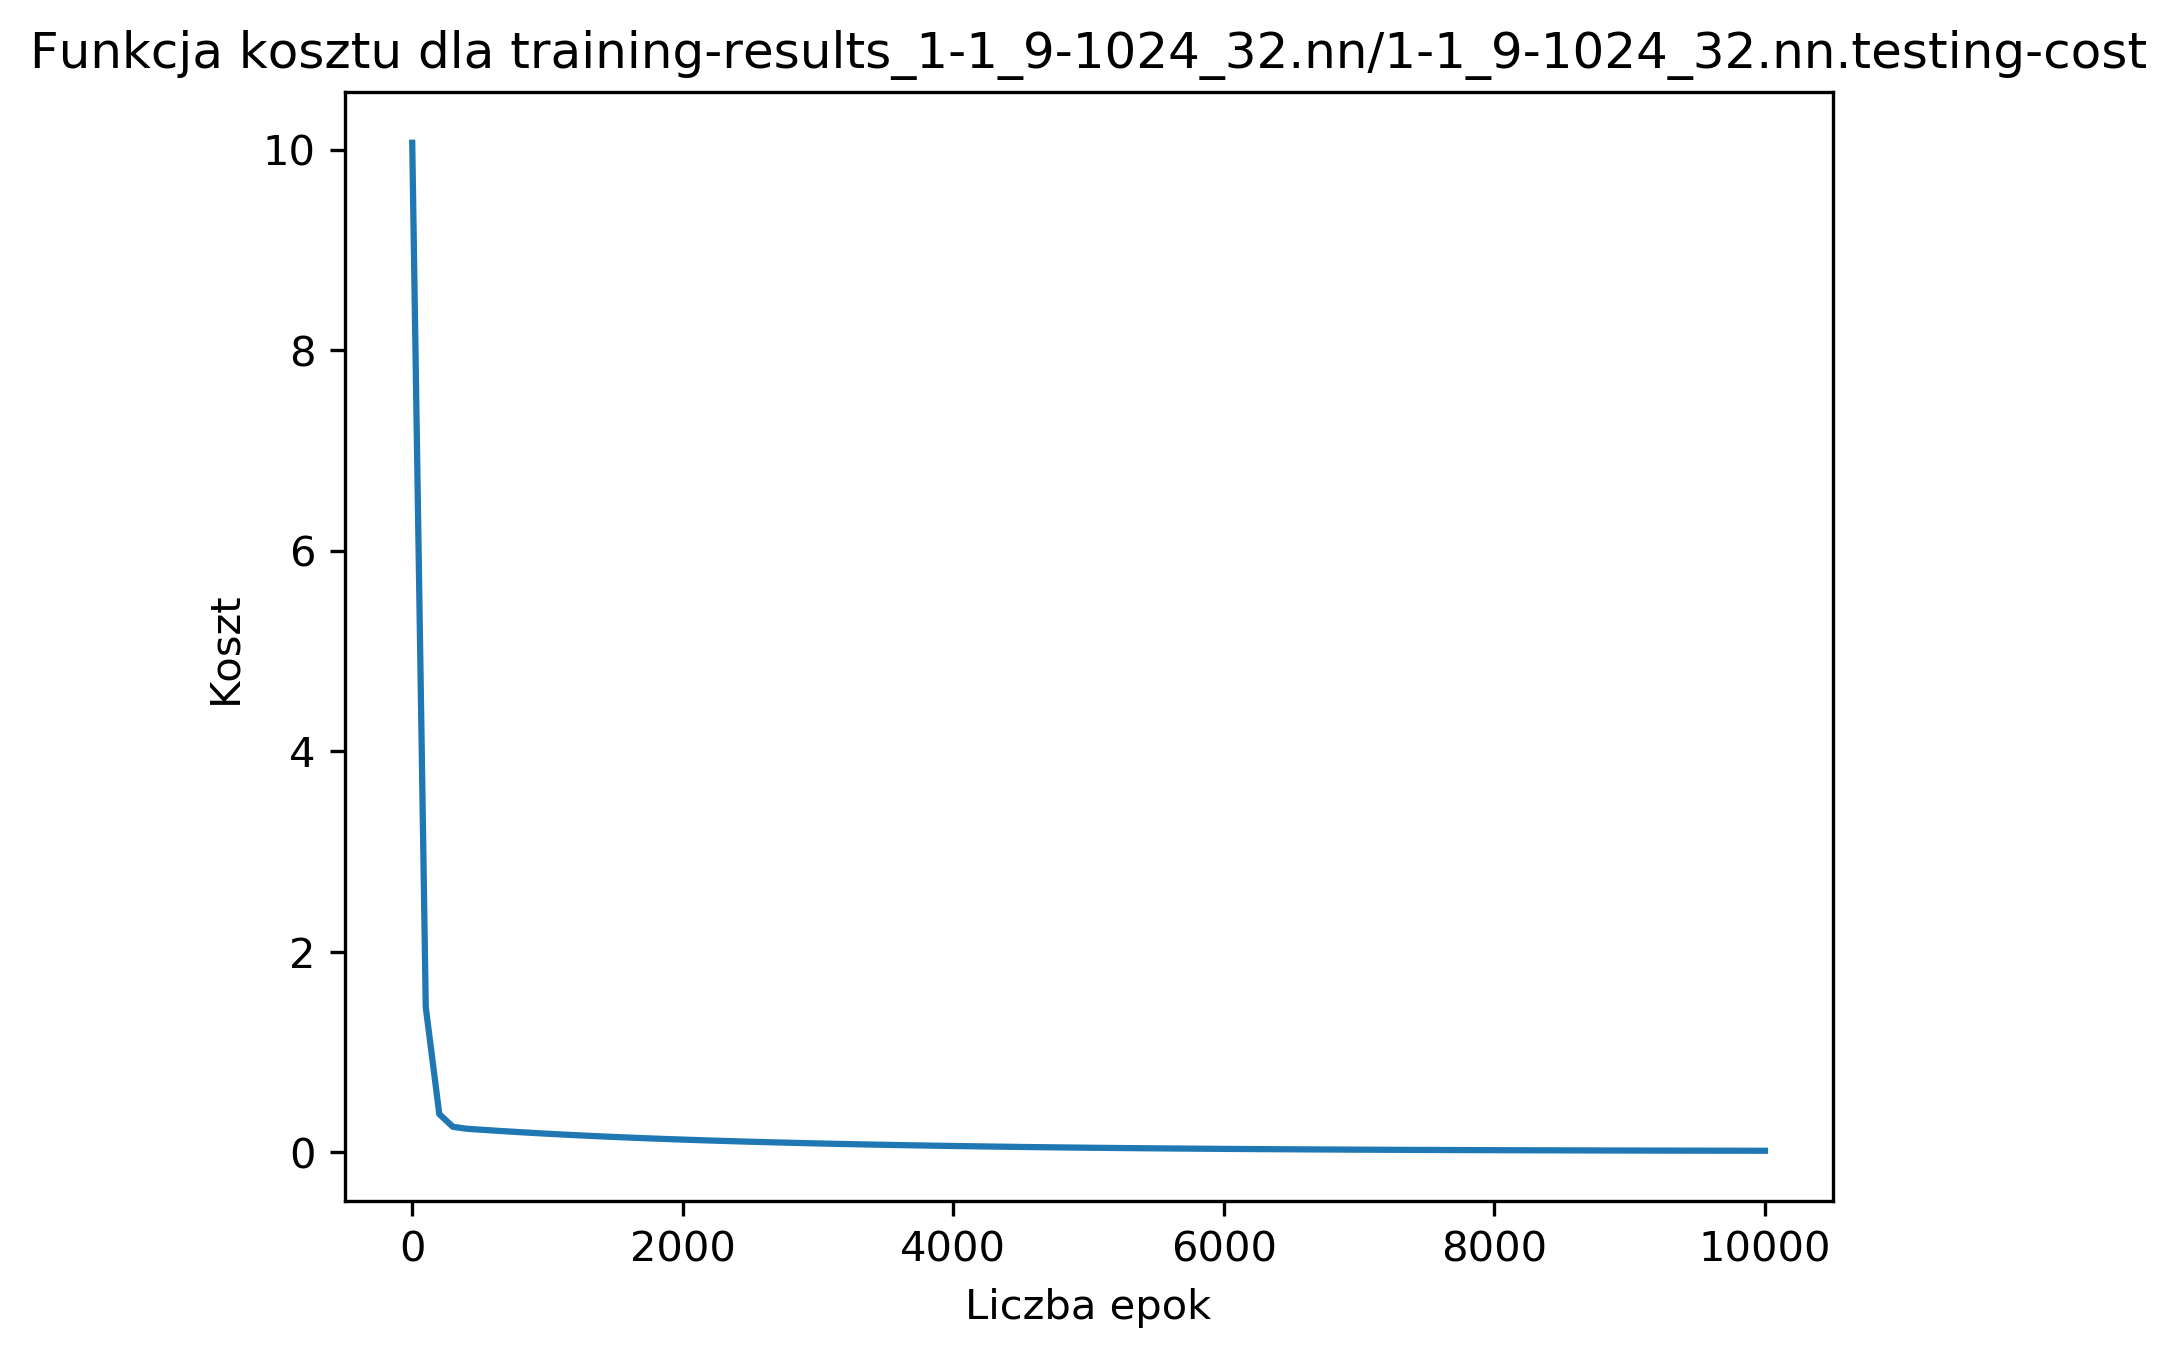
\includegraphics[width=120mm]{wykresy/1-1_9-1024_32_nn_testing-cost.png}
                \end{figure}
                \begin{figure}[!htbp]
                    \centering
                    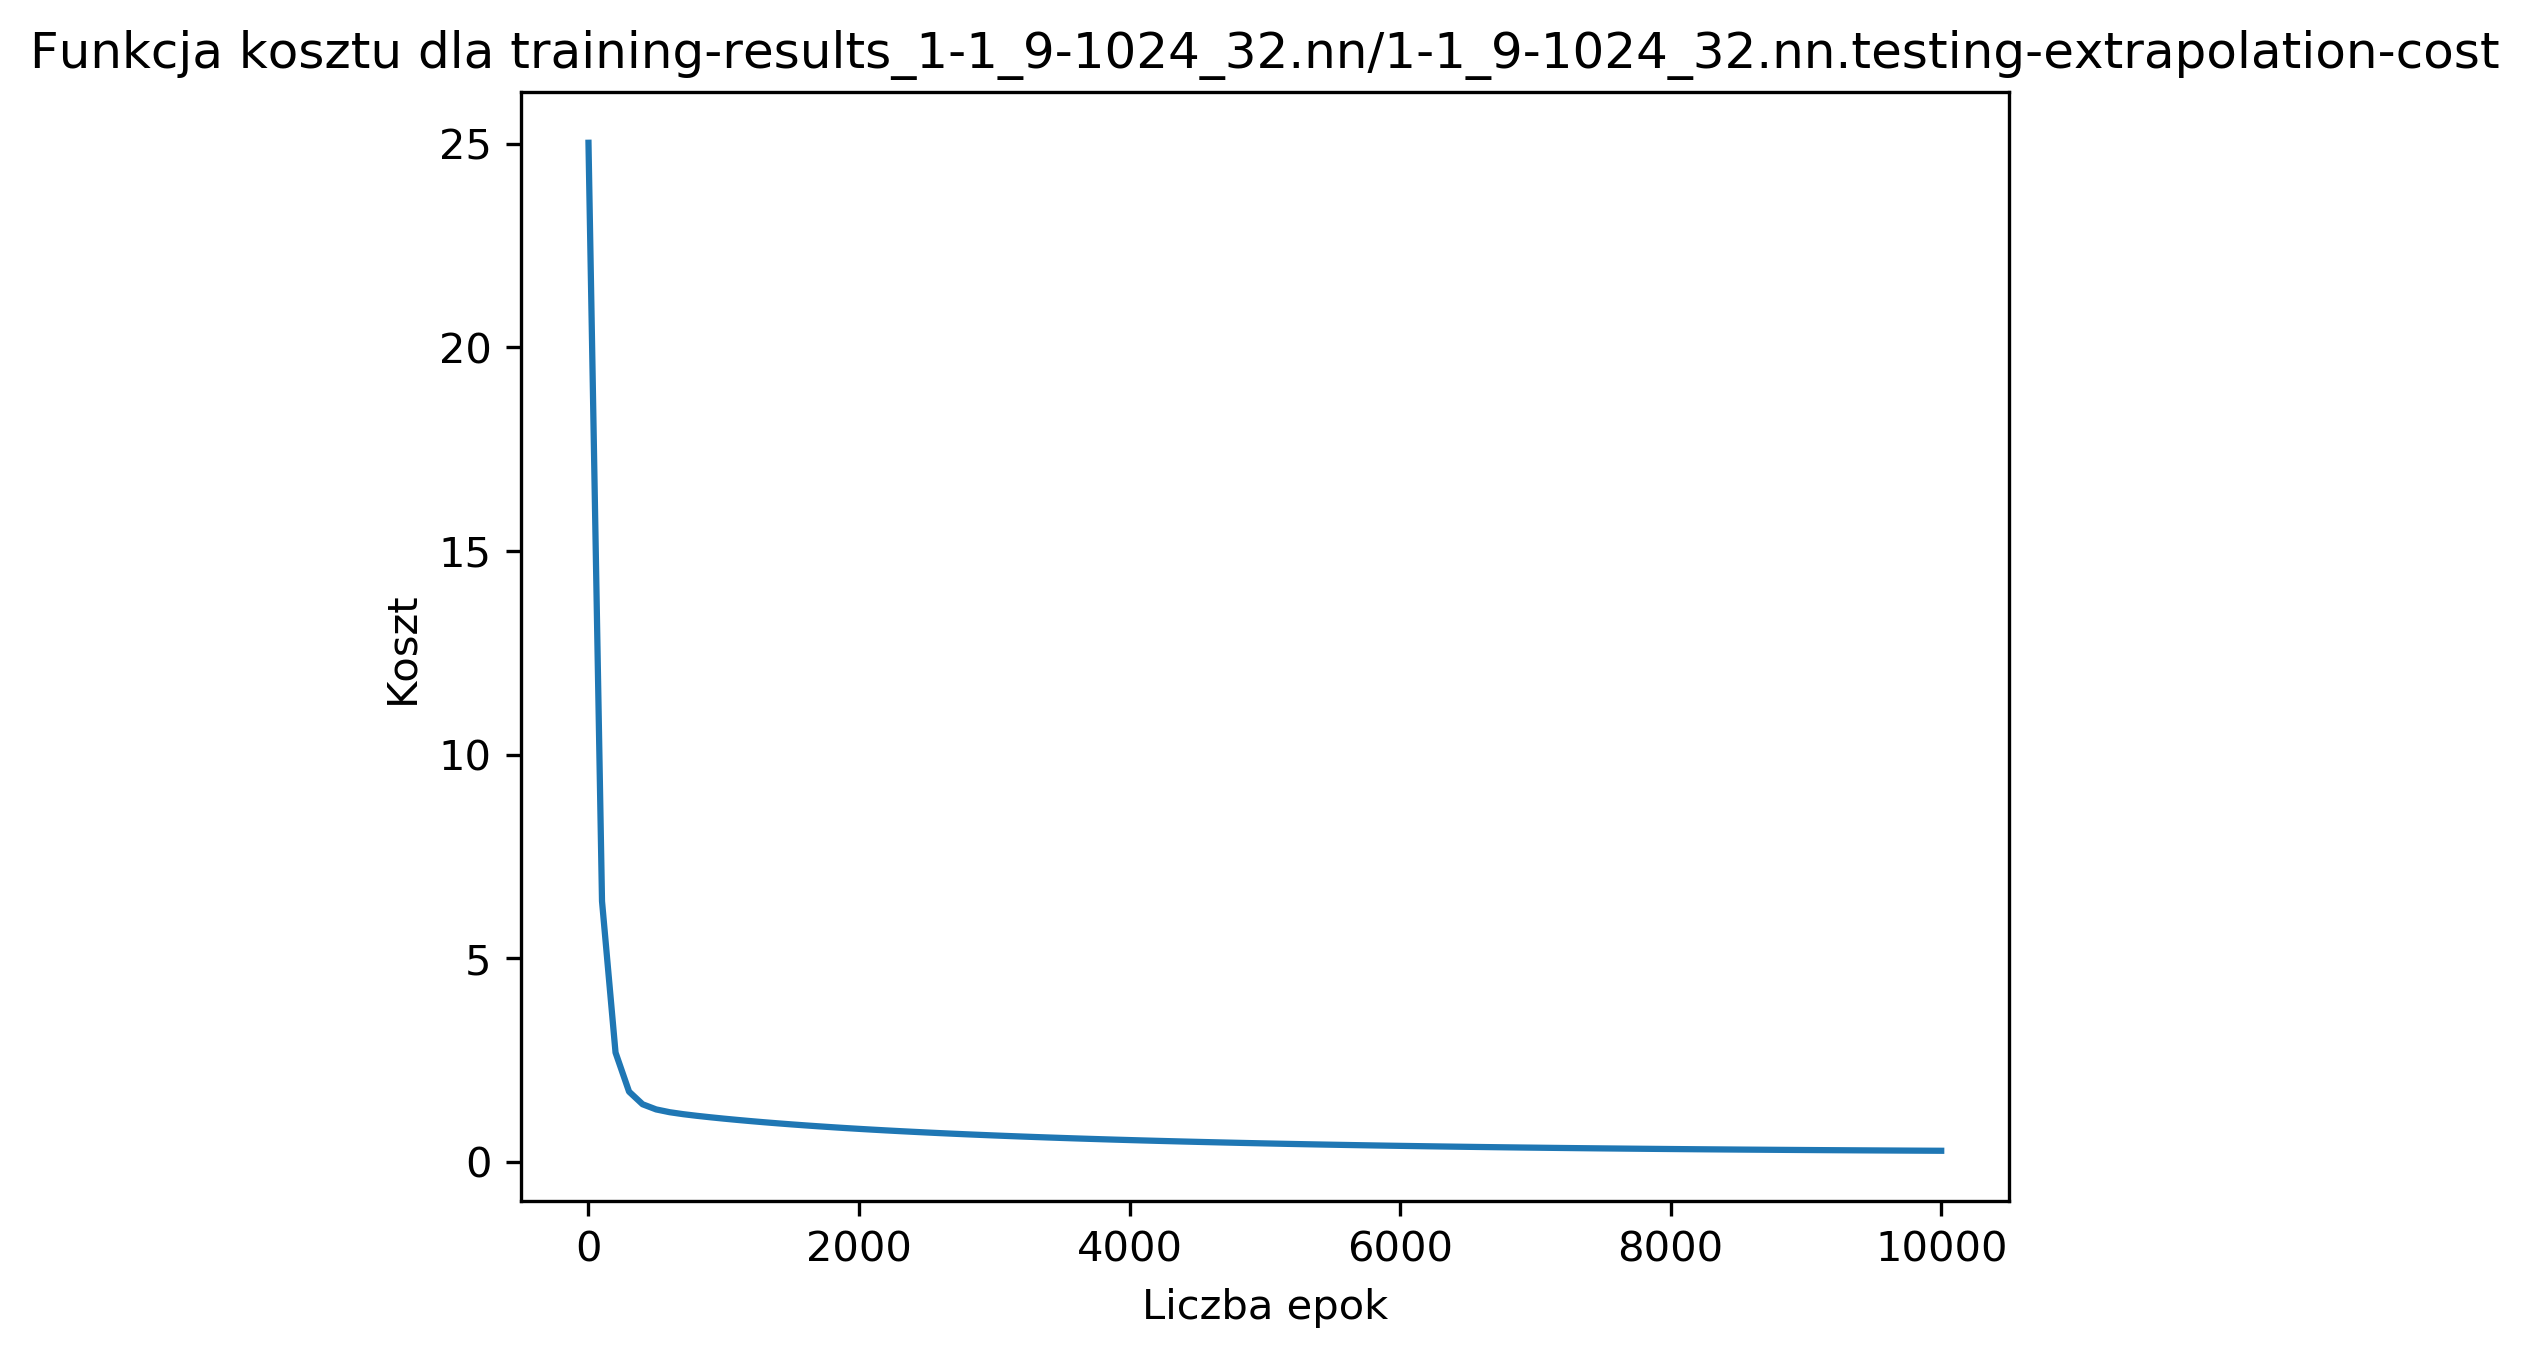
\includegraphics[width=140mm]{wykresy/1-1_9-1024_32_nn_testing-extrapolation-cost.png}
                \end{figure}
                \FloatBarrier
            %---------------------------------------------------%
                \begin{figure}[!htbp]
                    \centering
                    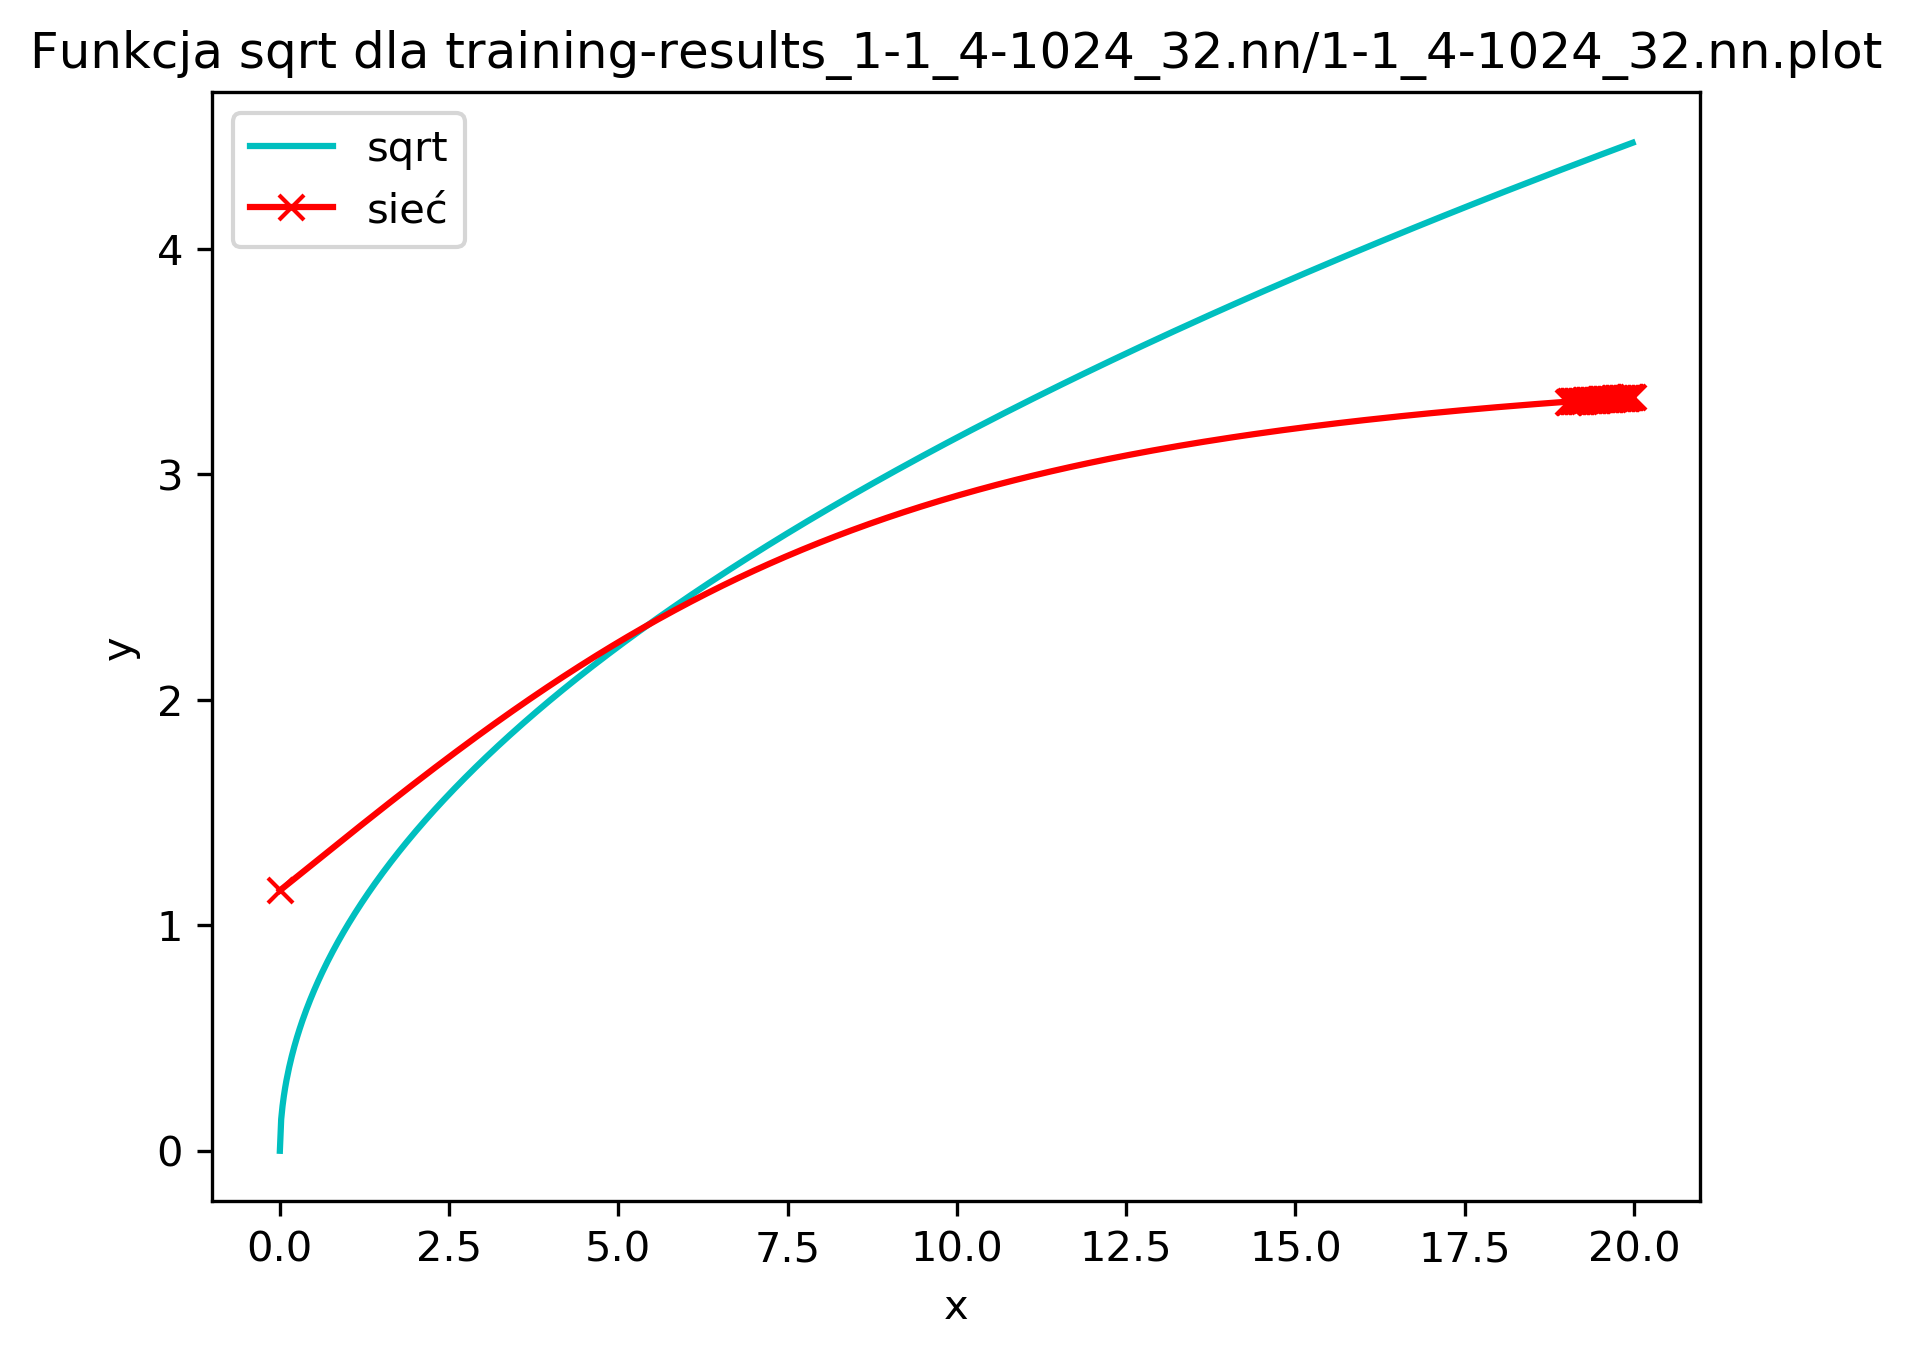
\includegraphics[width=105mm]{wykresy/1-1_4-1024_32_nn_plot.png}
                \end{figure}
                \begin{figure}[!htbp]
                    \centering
                    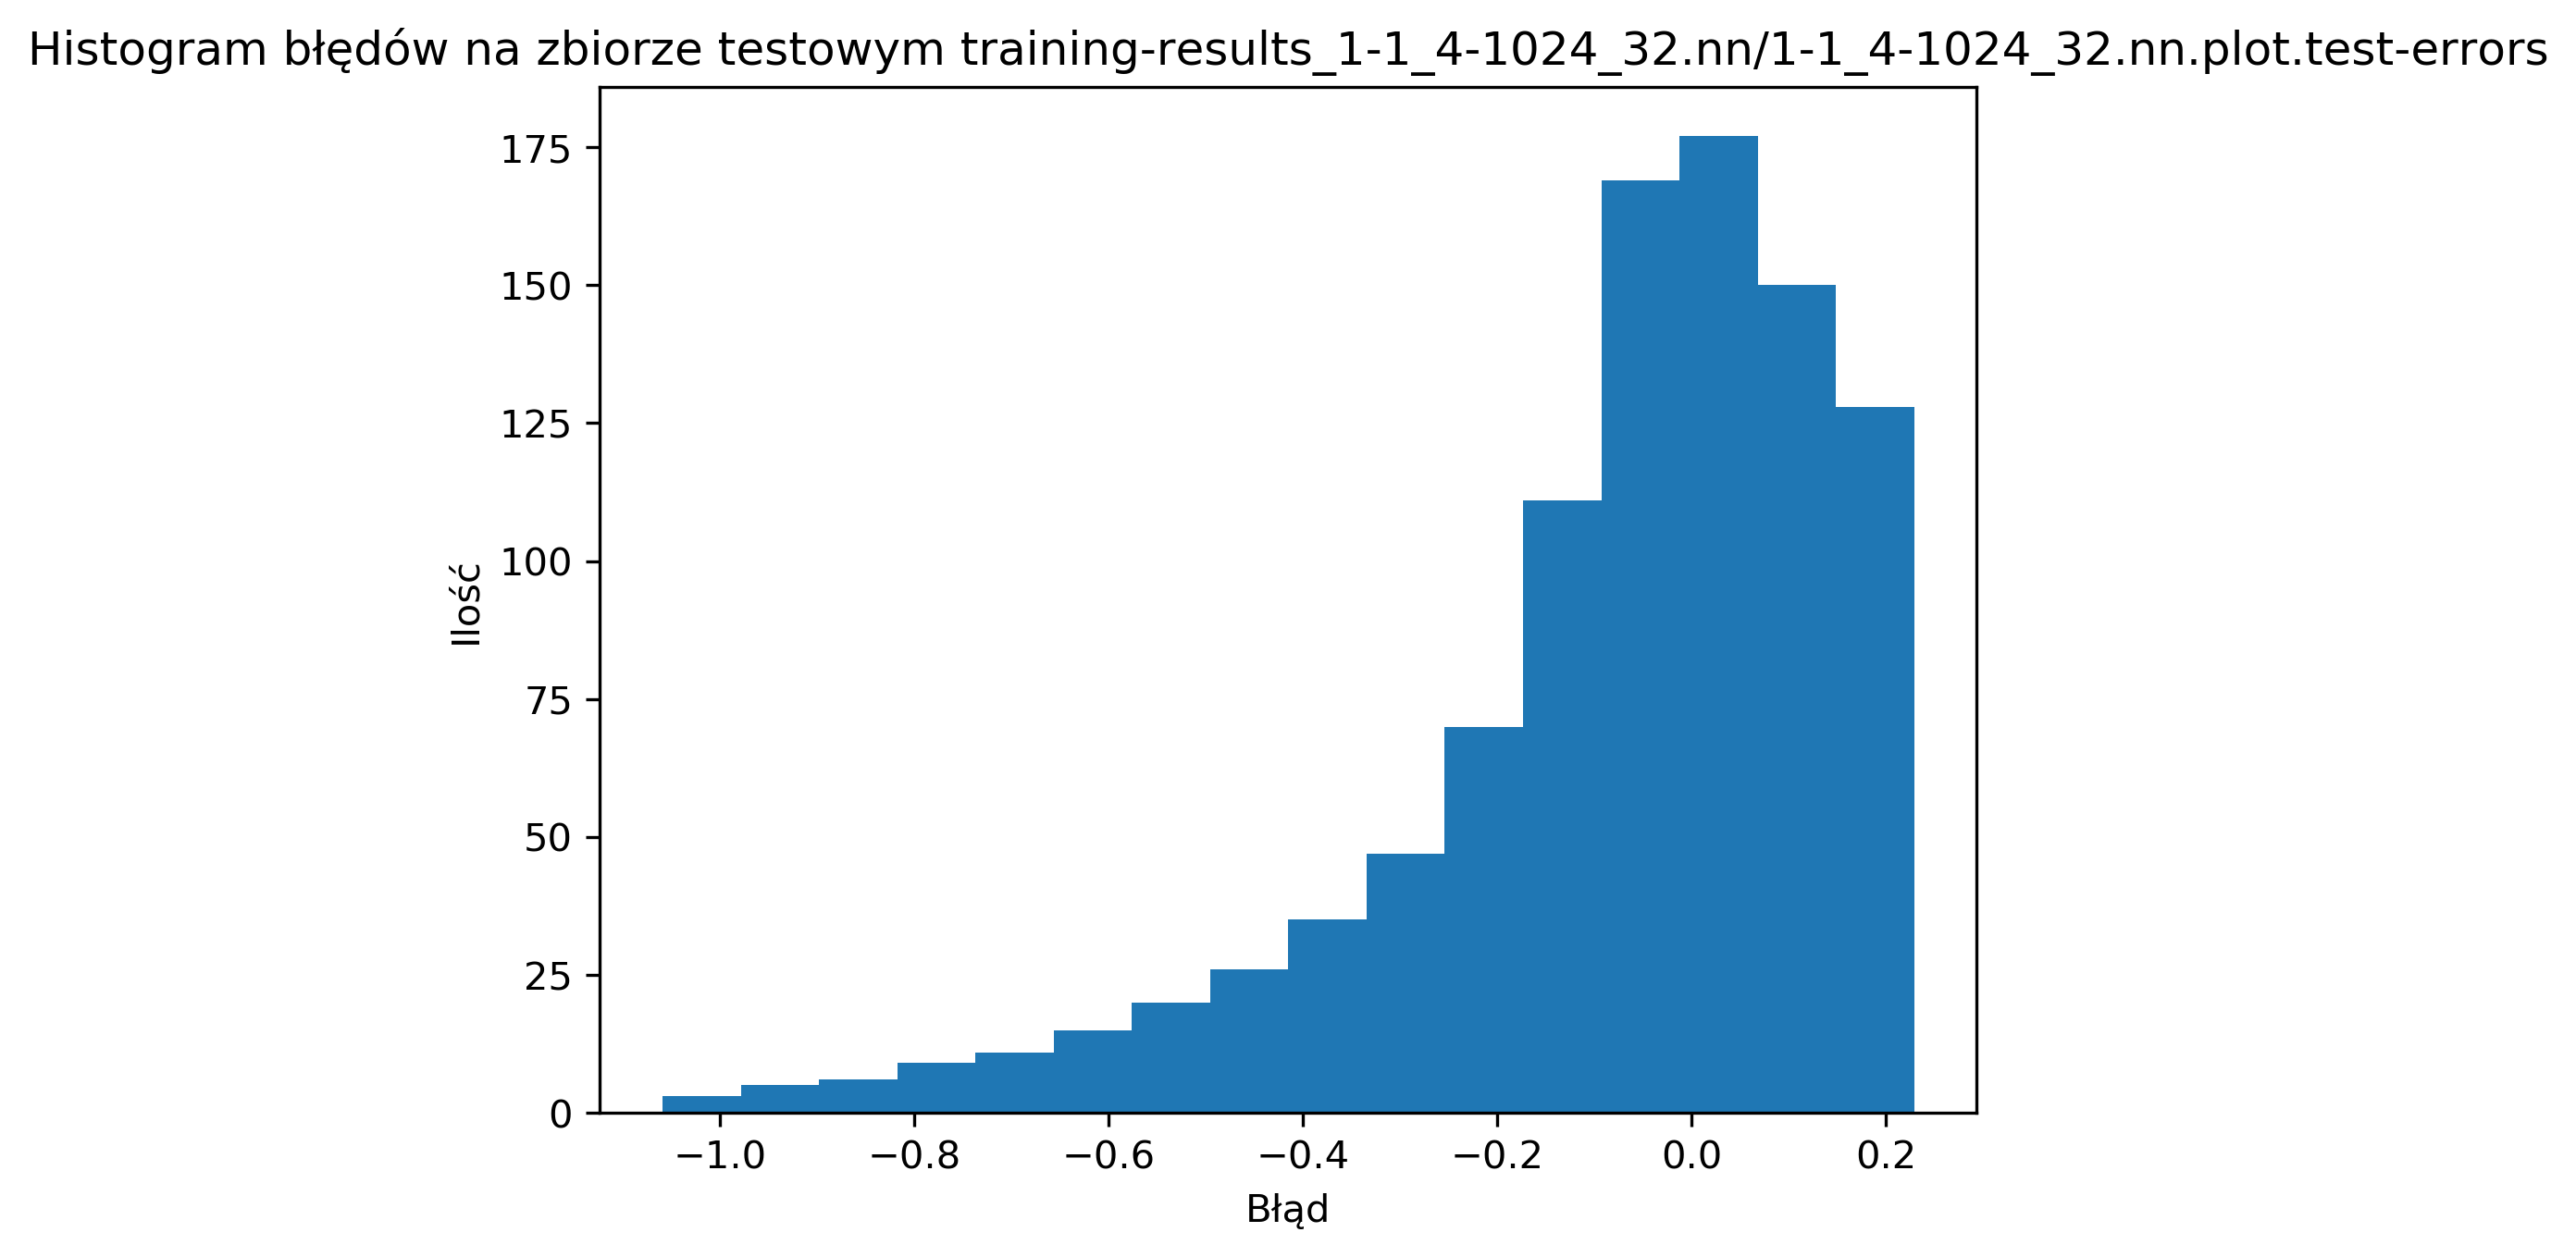
\includegraphics[width=140mm]{wykresy/1-1_4-1024_32_nn_plot_test-errors.png}
                \end{figure}
                \begin{figure}[!htbp]
                    \centering
                    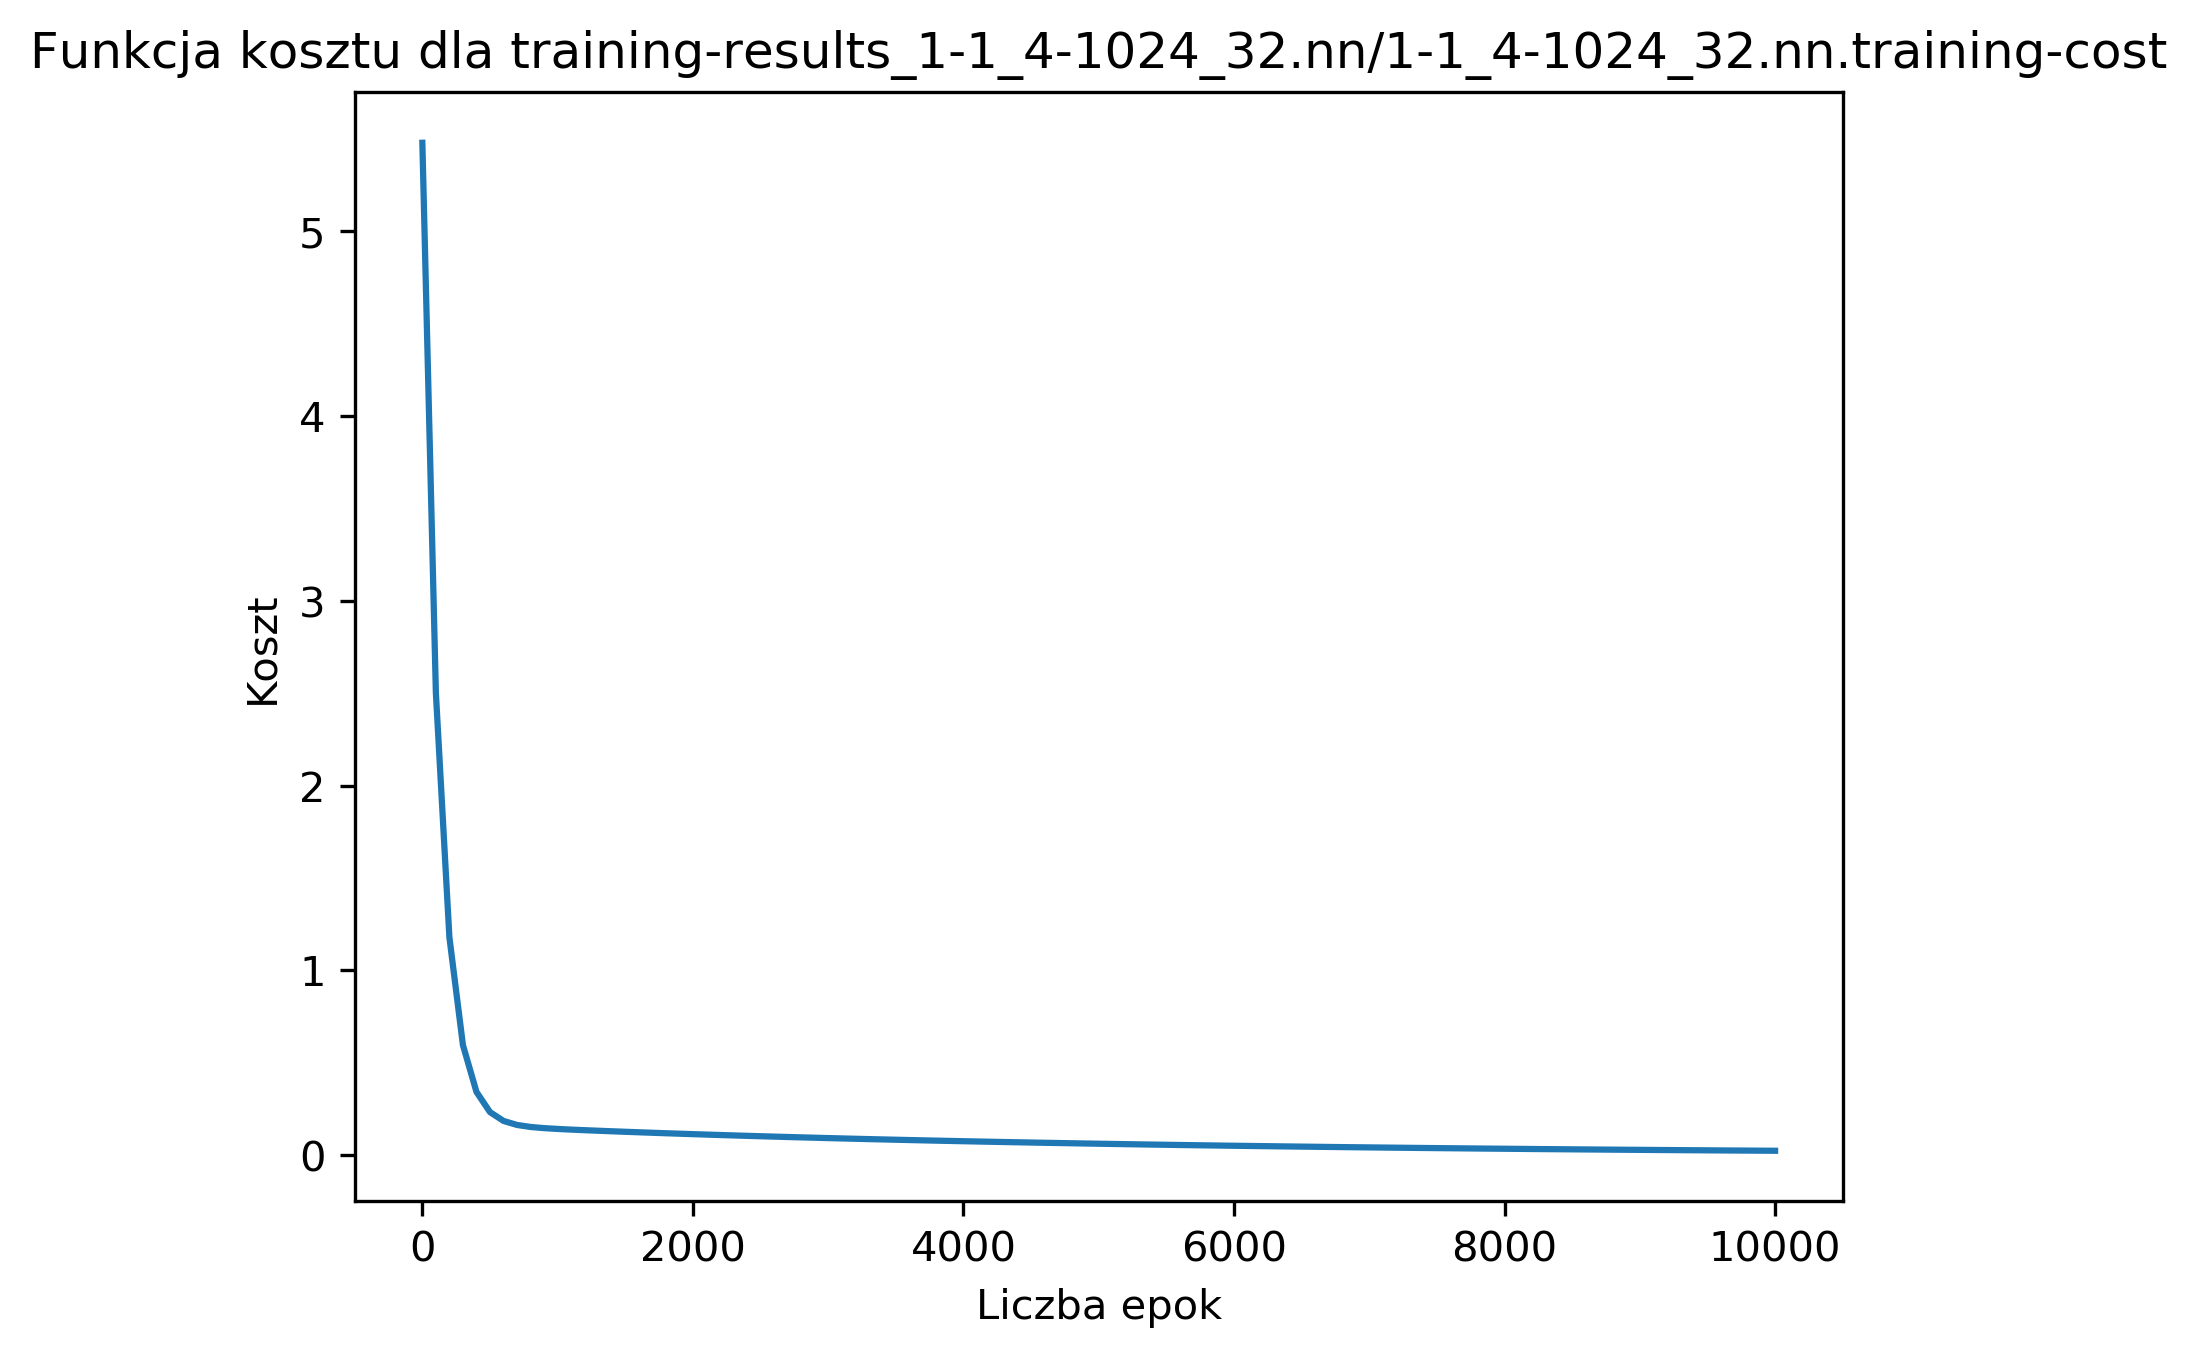
\includegraphics[width=140mm]{wykresy/1-1_4-1024_32_nn_training-cost.png}
                \end{figure}
                \begin{figure}[!htbp]
                    \centering
                    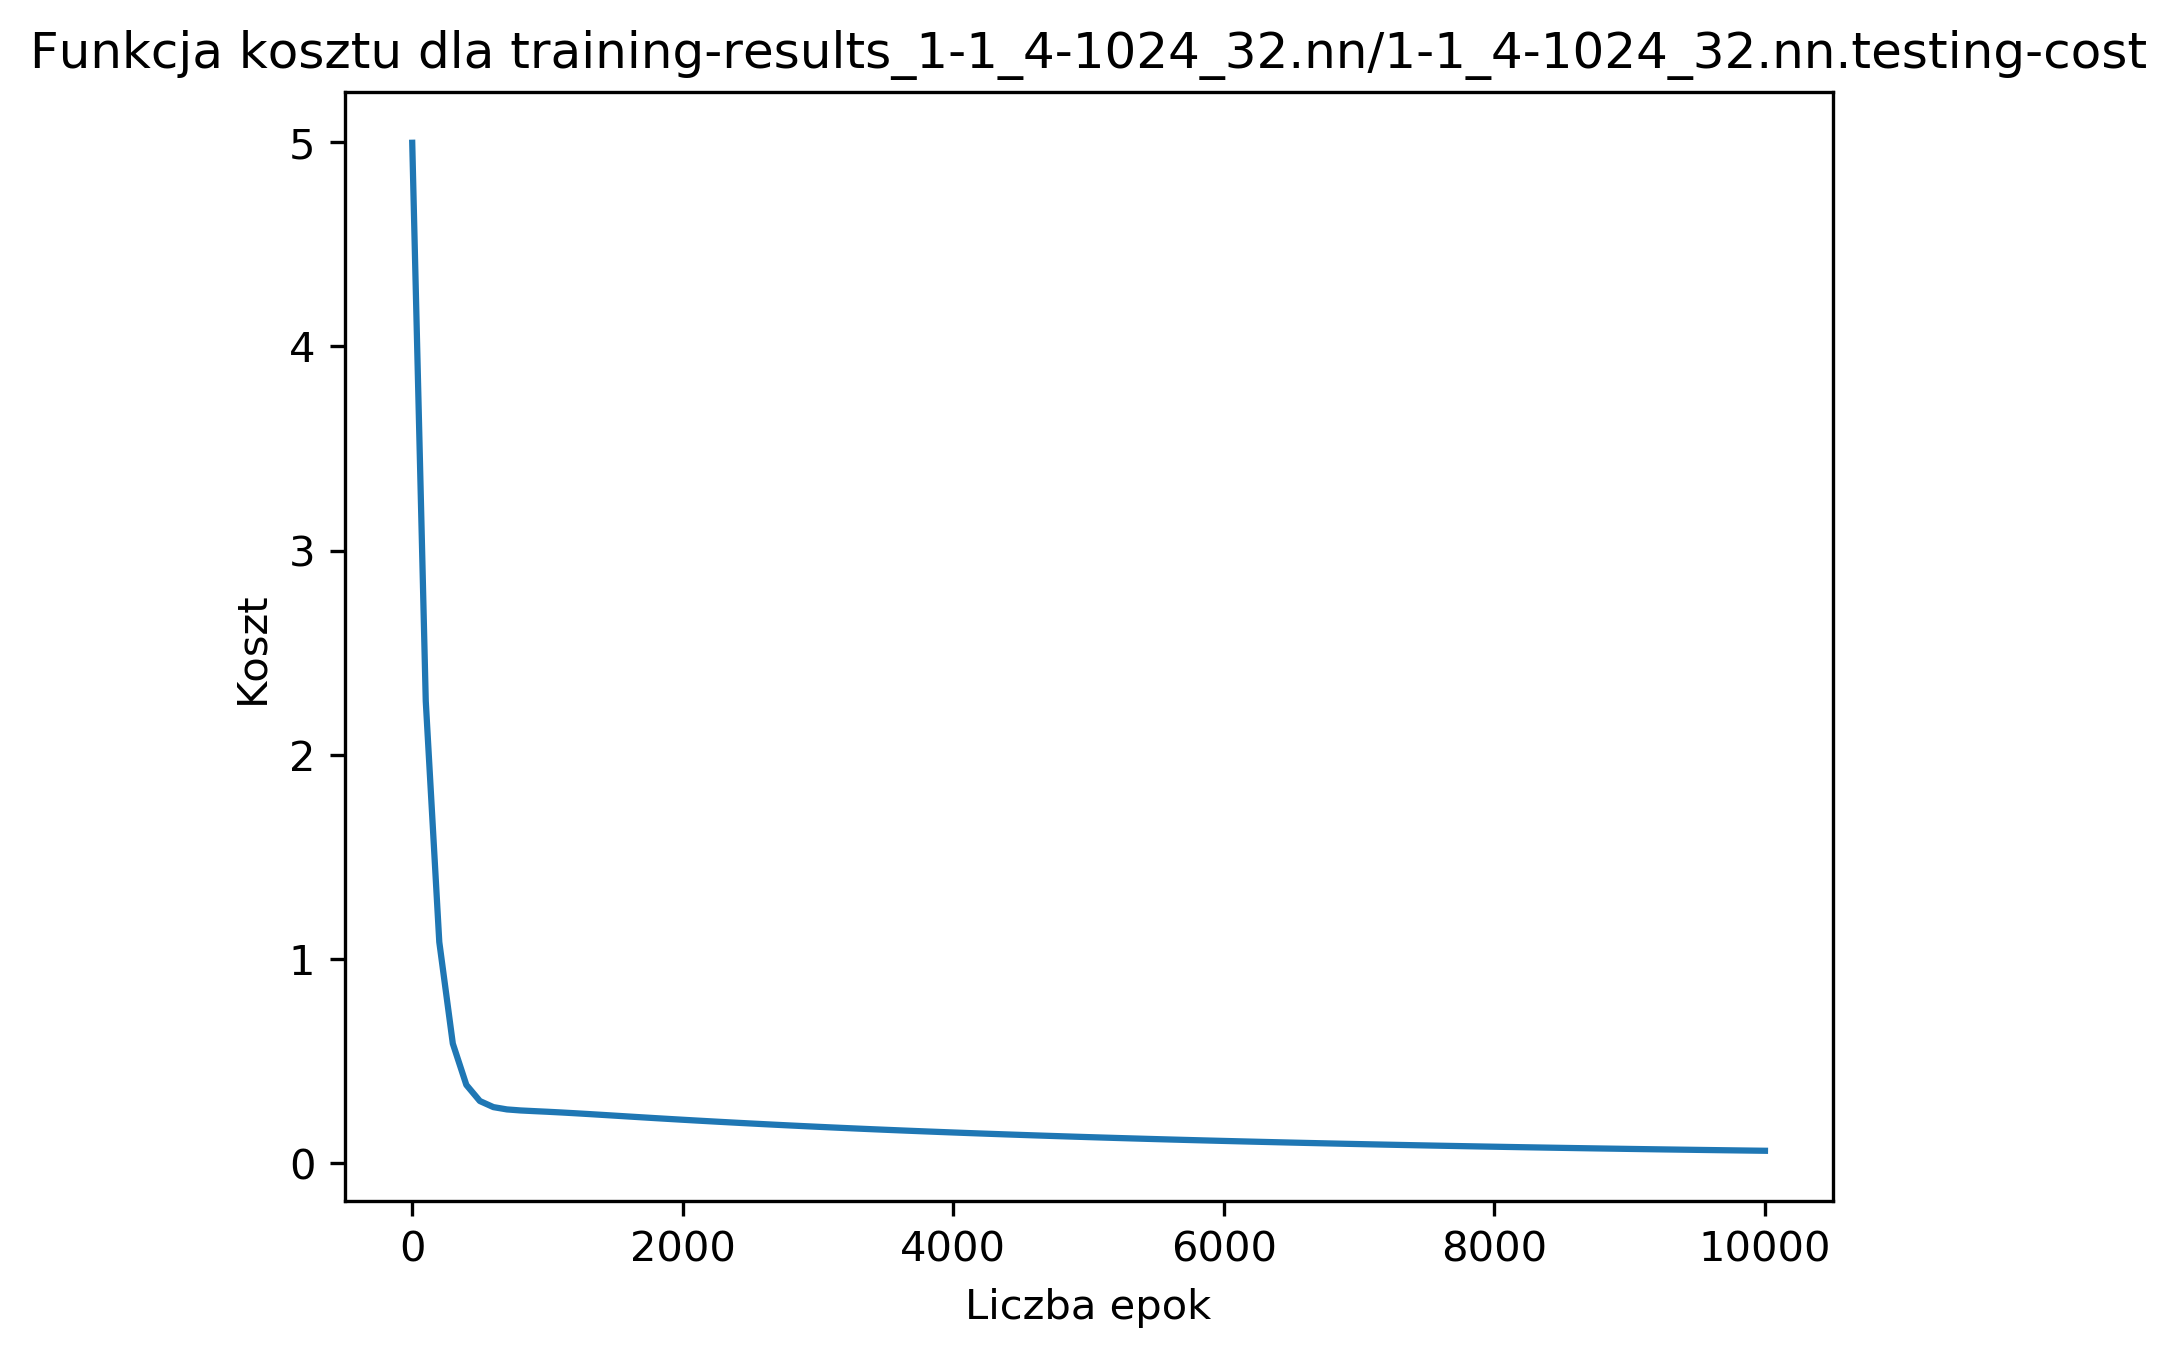
\includegraphics[width=120mm]{wykresy/1-1_4-1024_32_nn_testing-cost.png}
                \end{figure}
                \begin{figure}[!htbp]
                    \centering
                    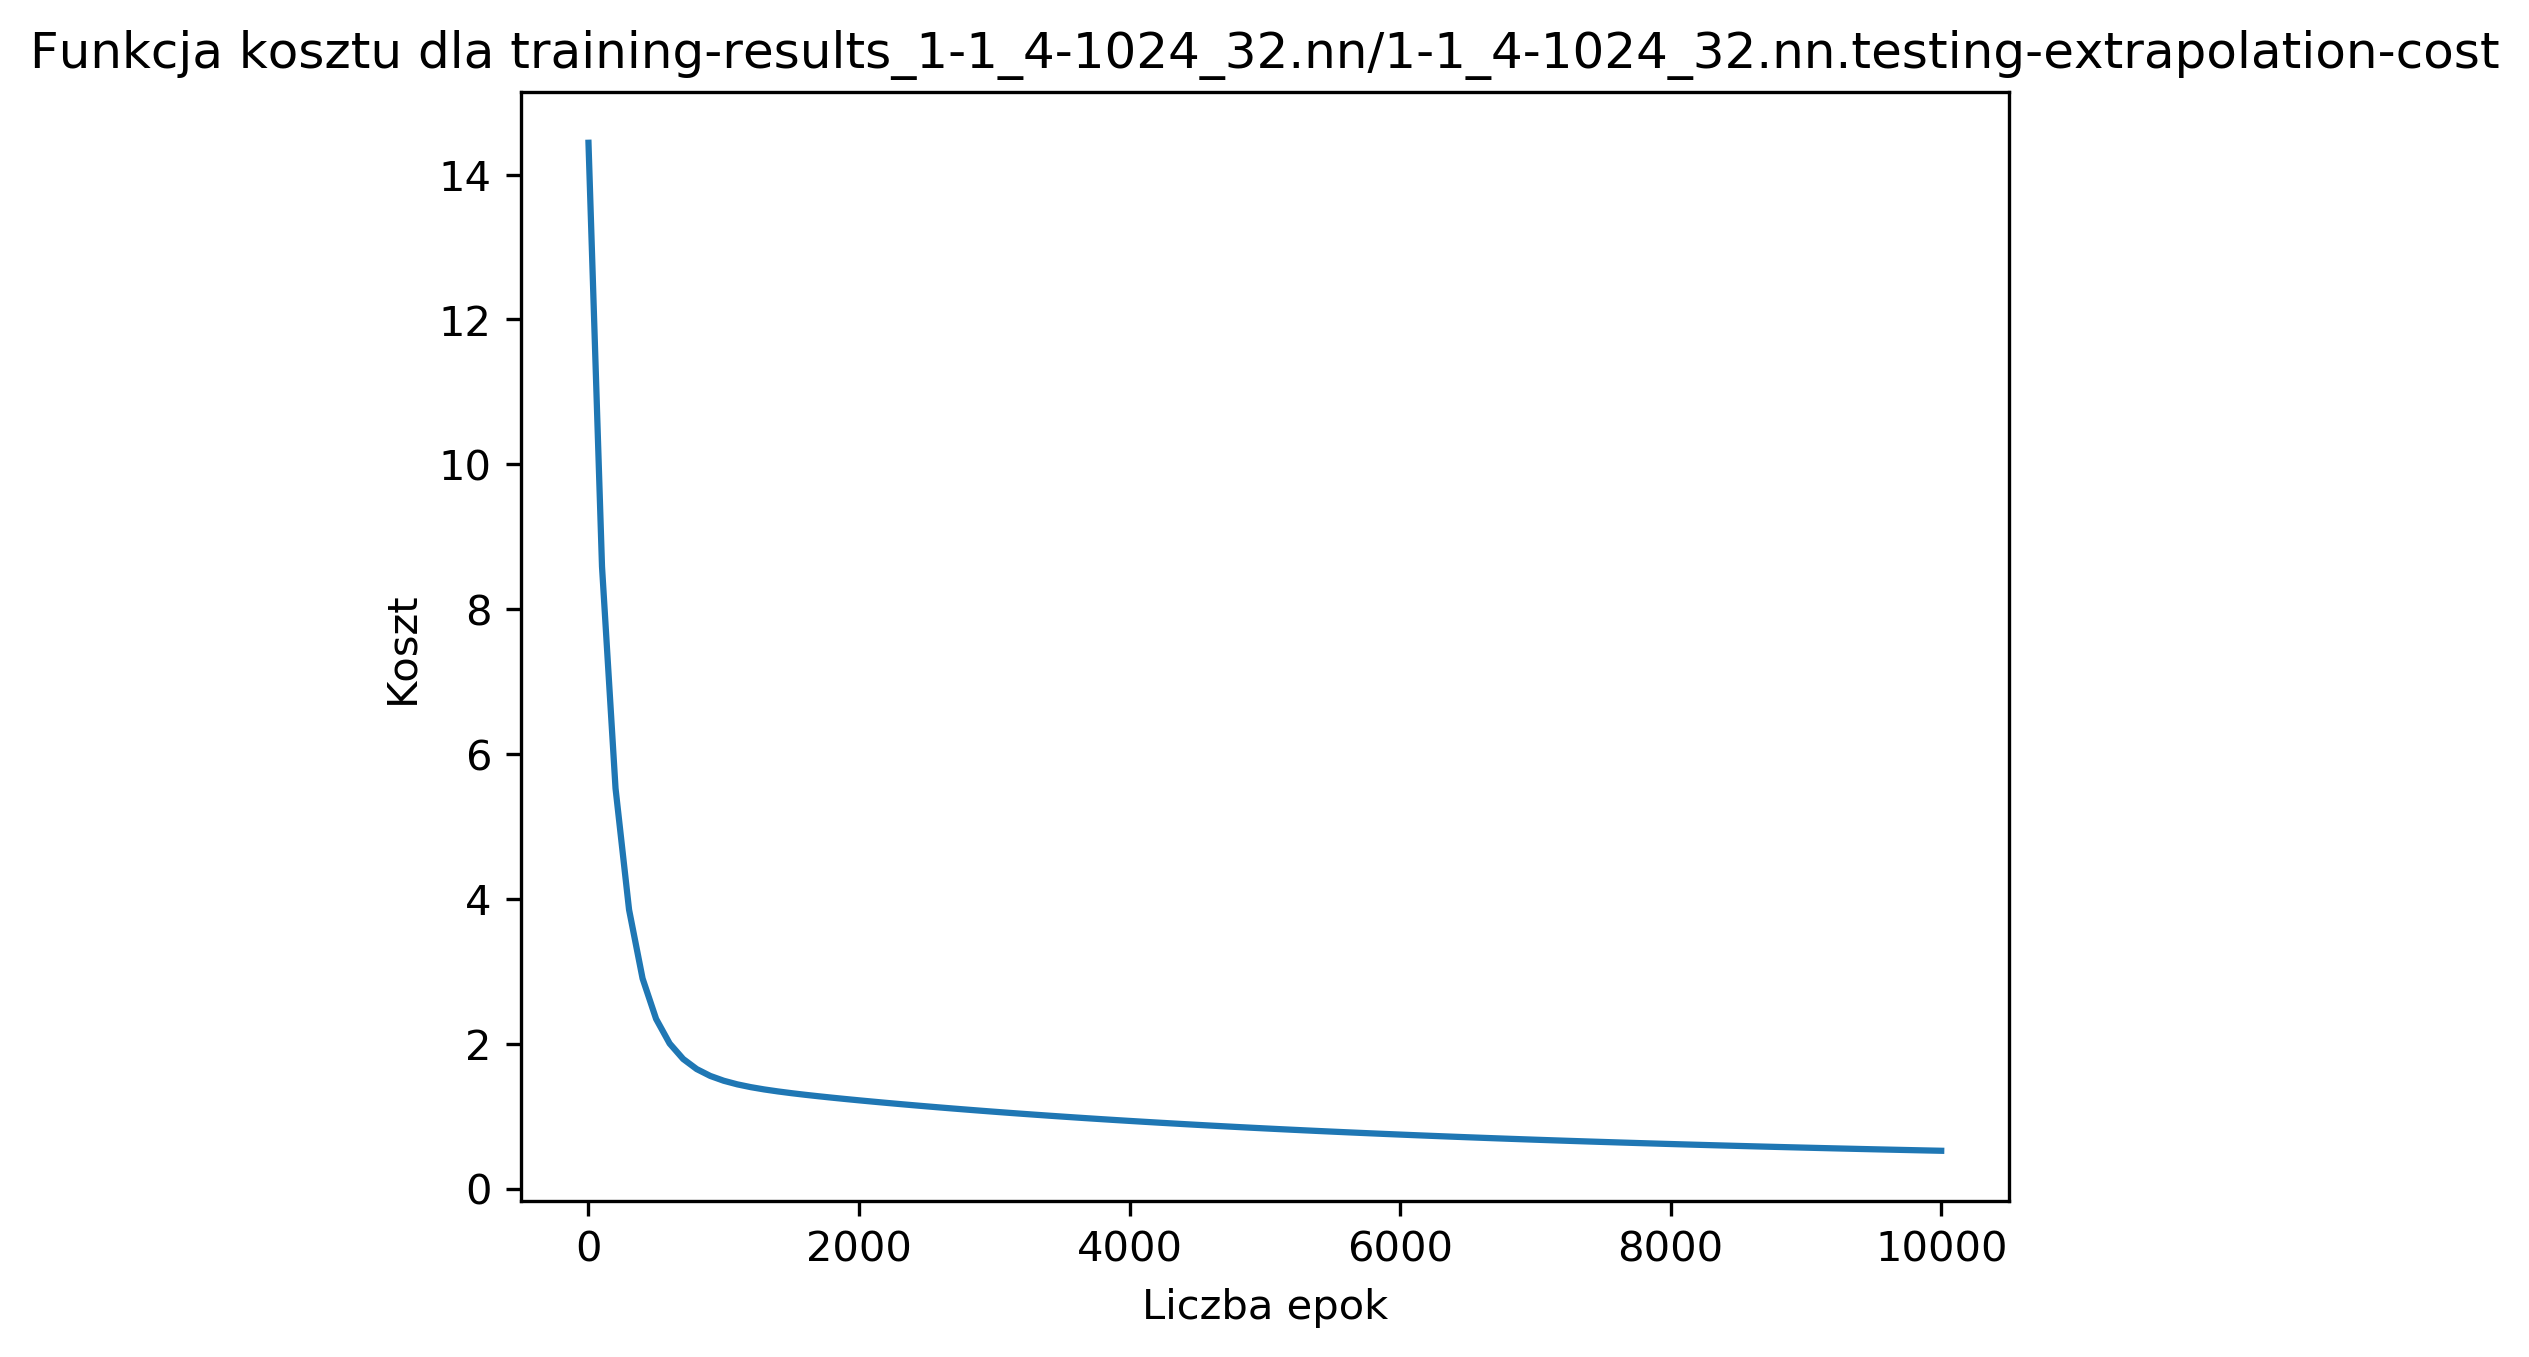
\includegraphics[width=120mm]{wykresy/1-1_4-1024_32_nn_testing-extrapolation-cost.png}
                \end{figure}
                \FloatBarrier
            %---------------------------------------------------%
            }
        }
    %---------------------------------------------------%
        \subsection{Funkcja sinusa - sin}
        {
            \begin{figure}[!htbp]
                \centering
                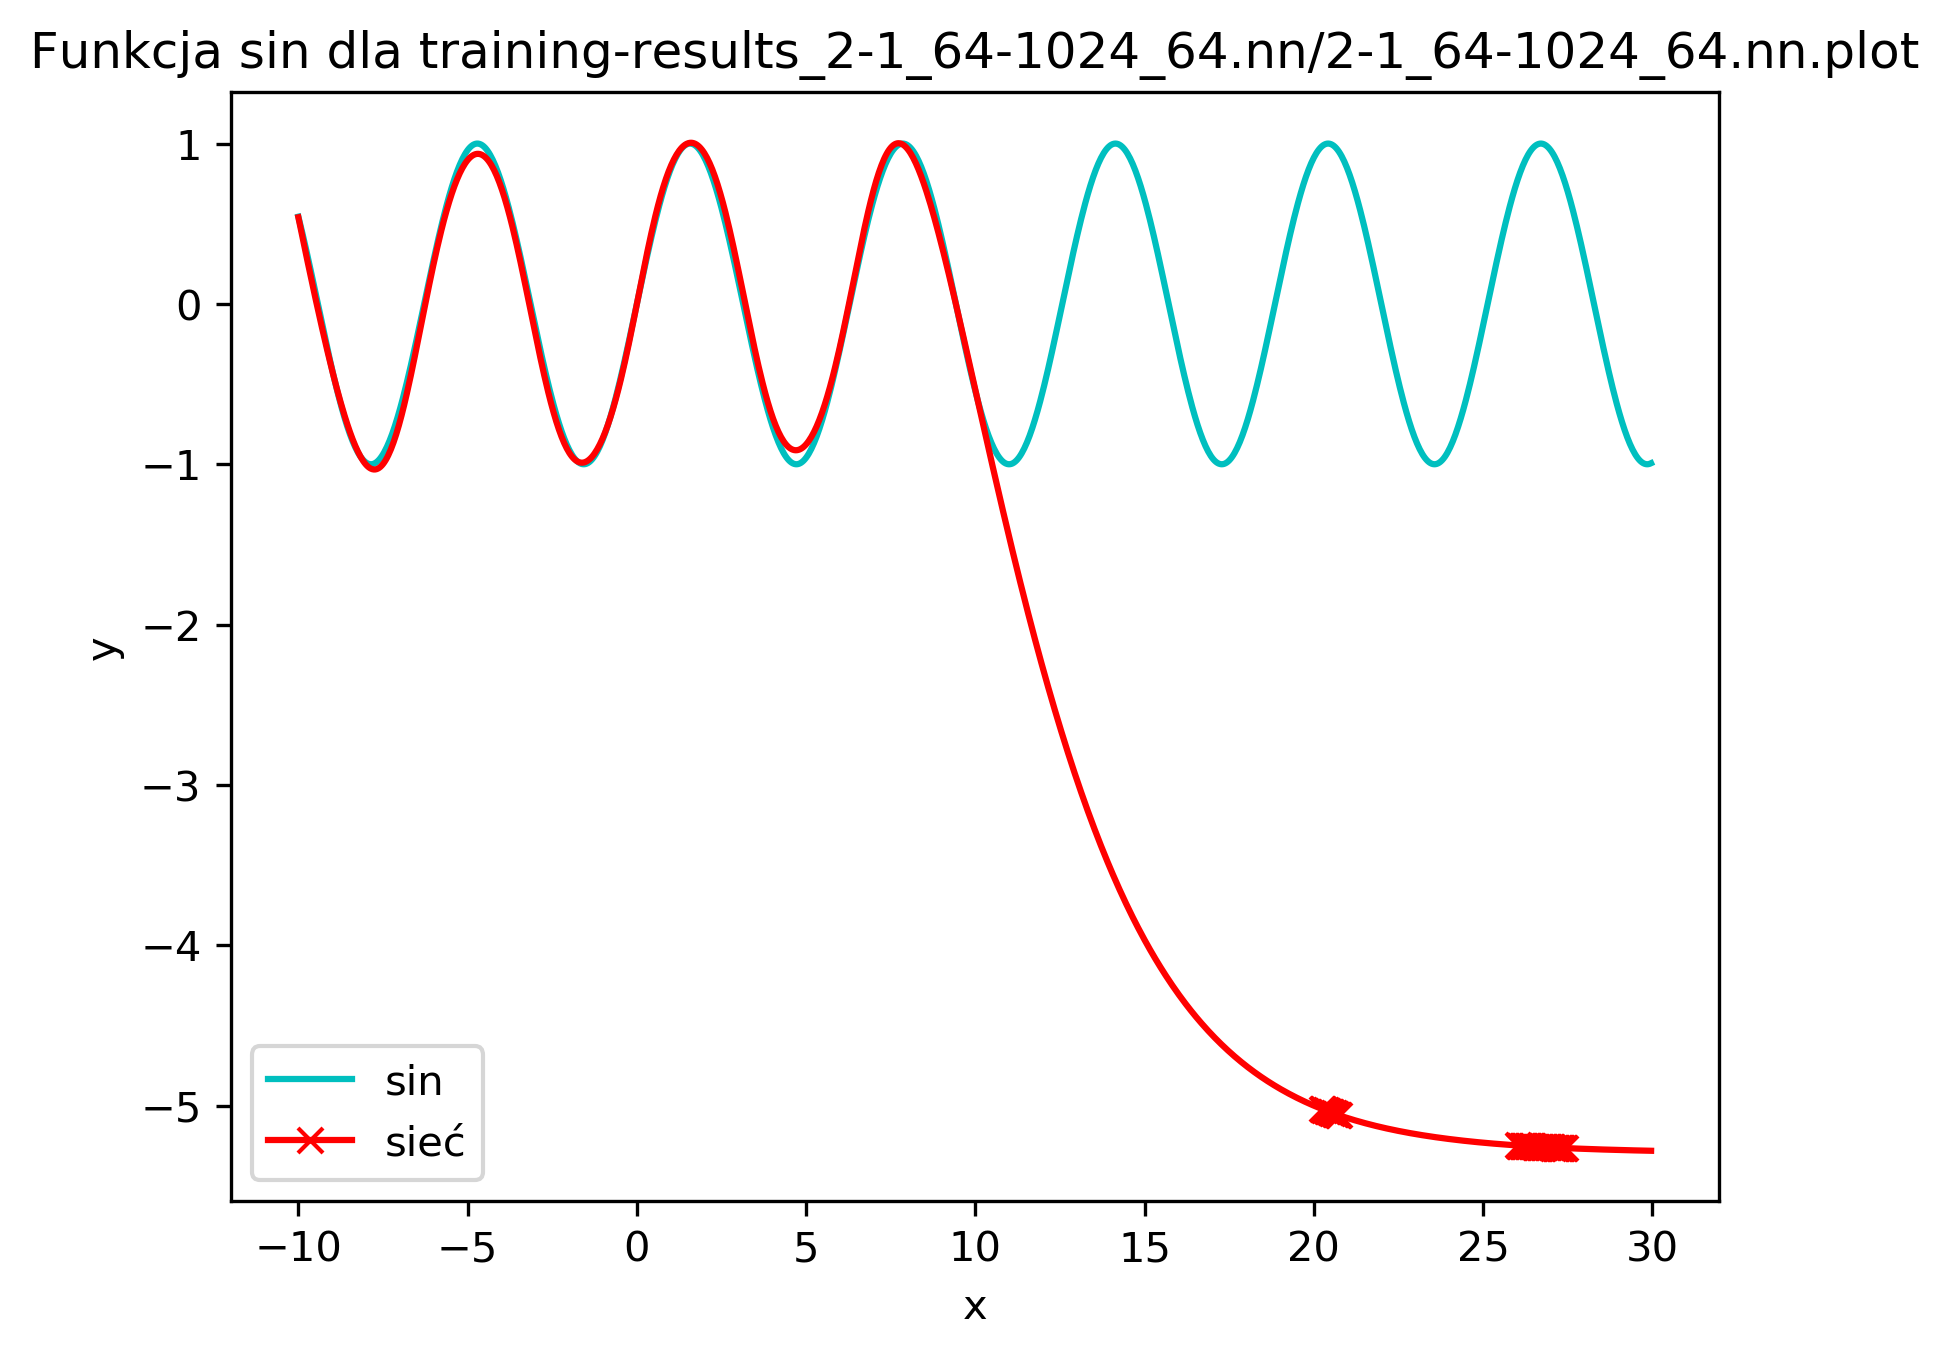
\includegraphics[width=105mm]{wykresy/2-1_64-1024_64_nn_plot.png}
            \end{figure}
            \begin{figure}[!htbp]
                \centering
                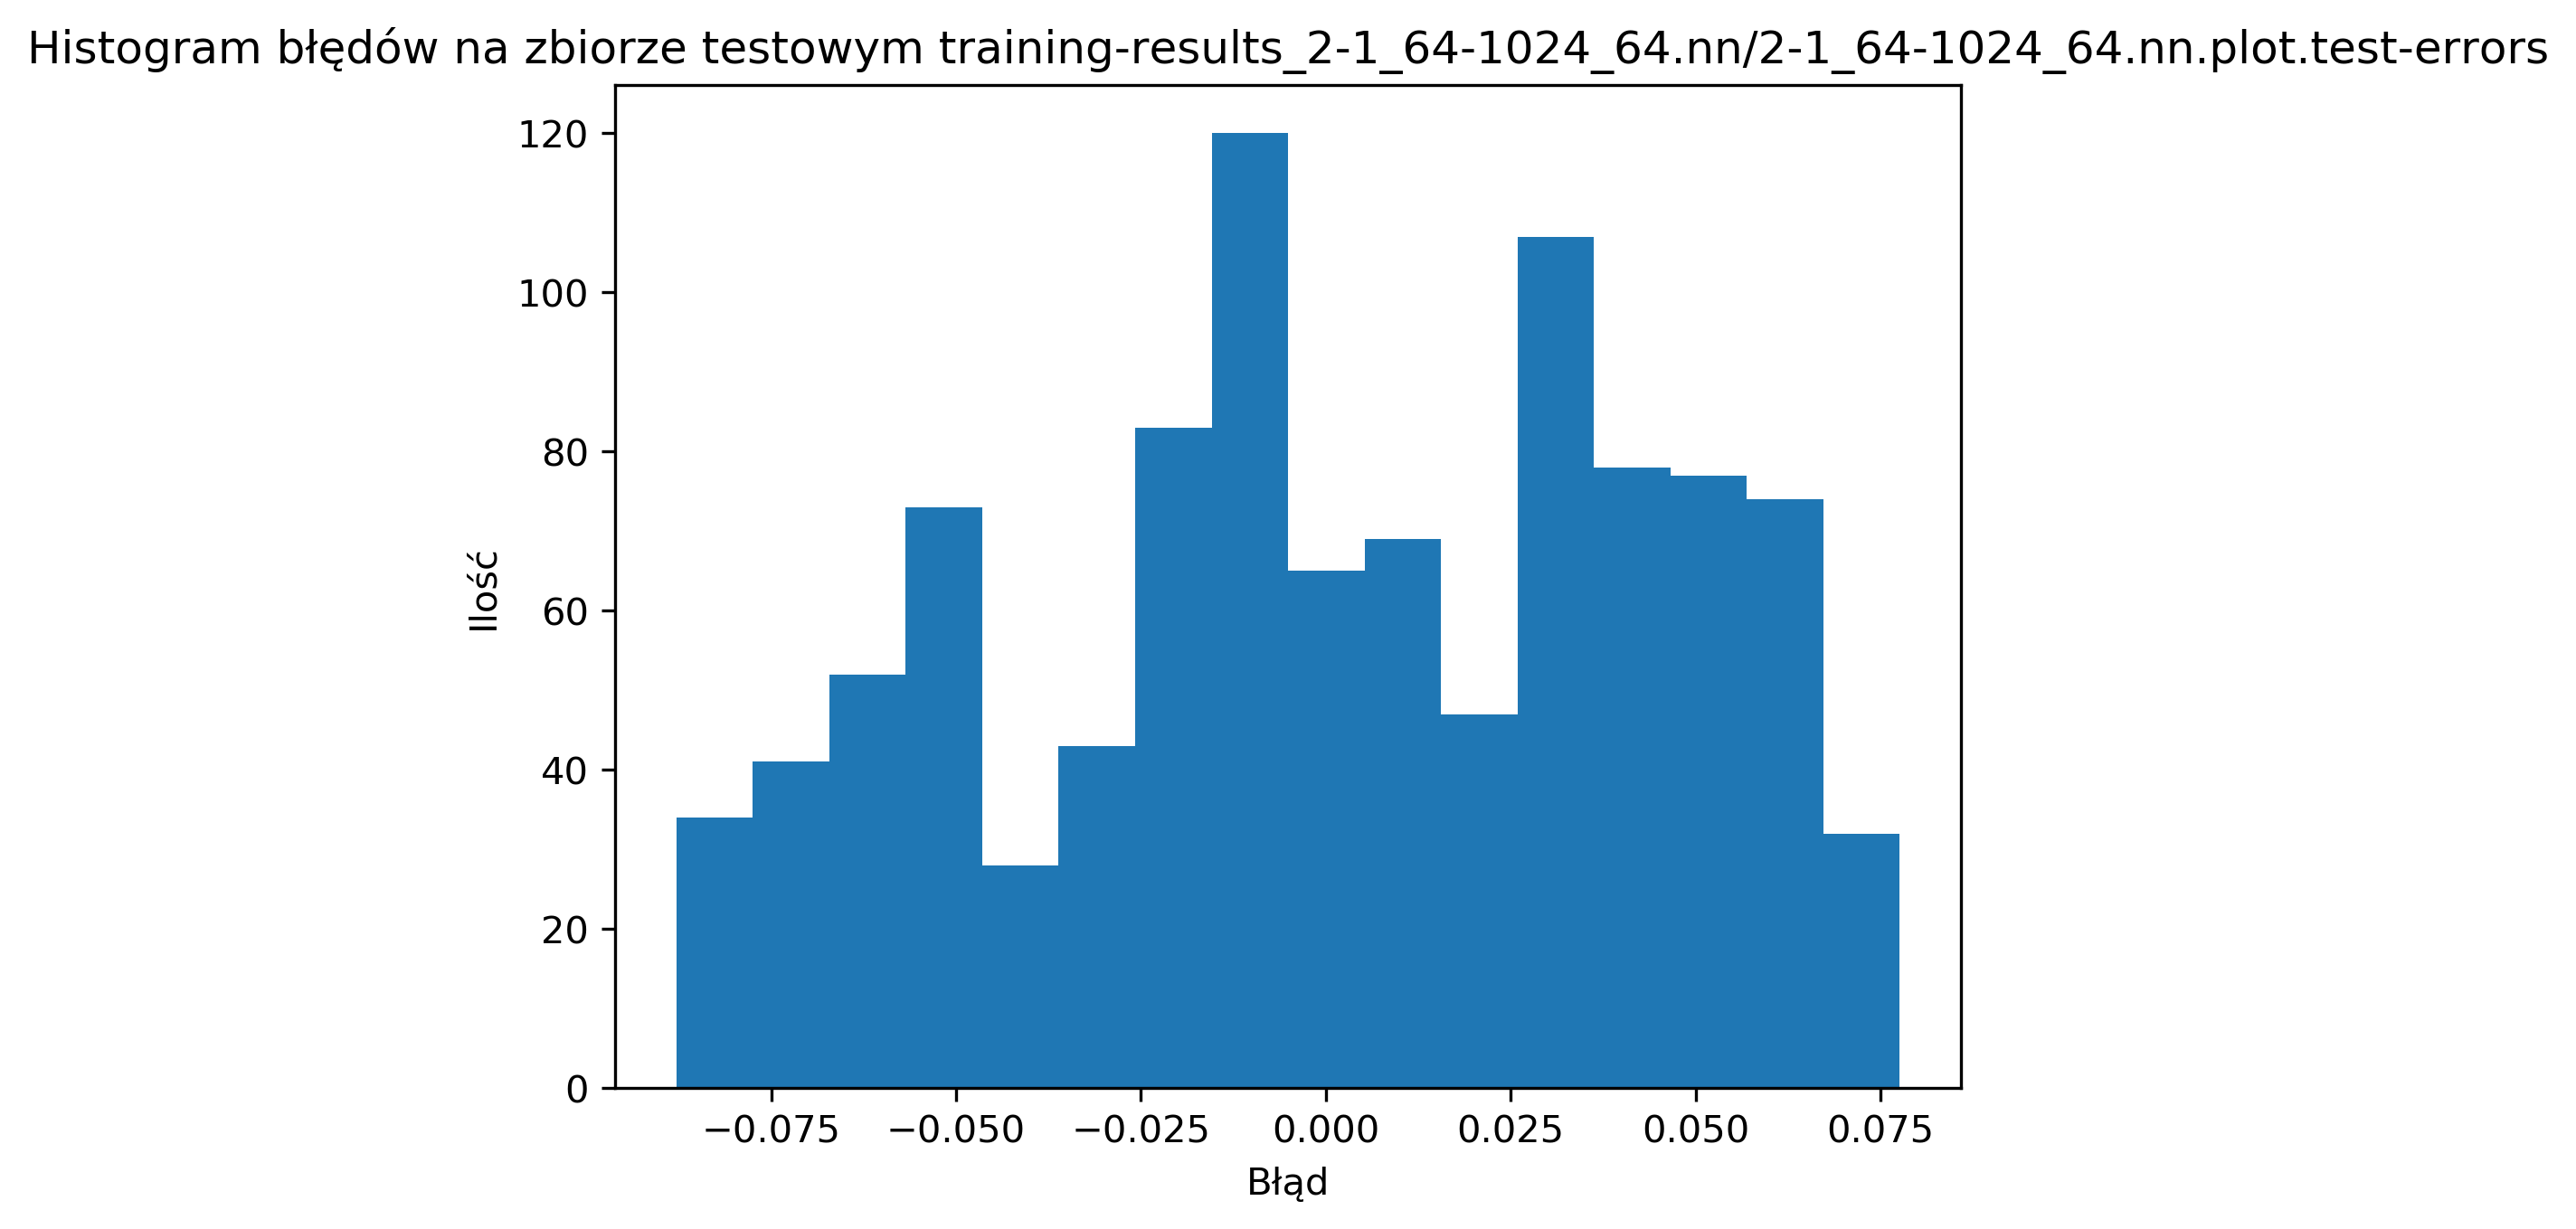
\includegraphics[width=140mm]{wykresy/2-1_64-1024_64_nn_plot_test-errors.png}
            \end{figure}
            \begin{figure}[!htbp]
                \centering
                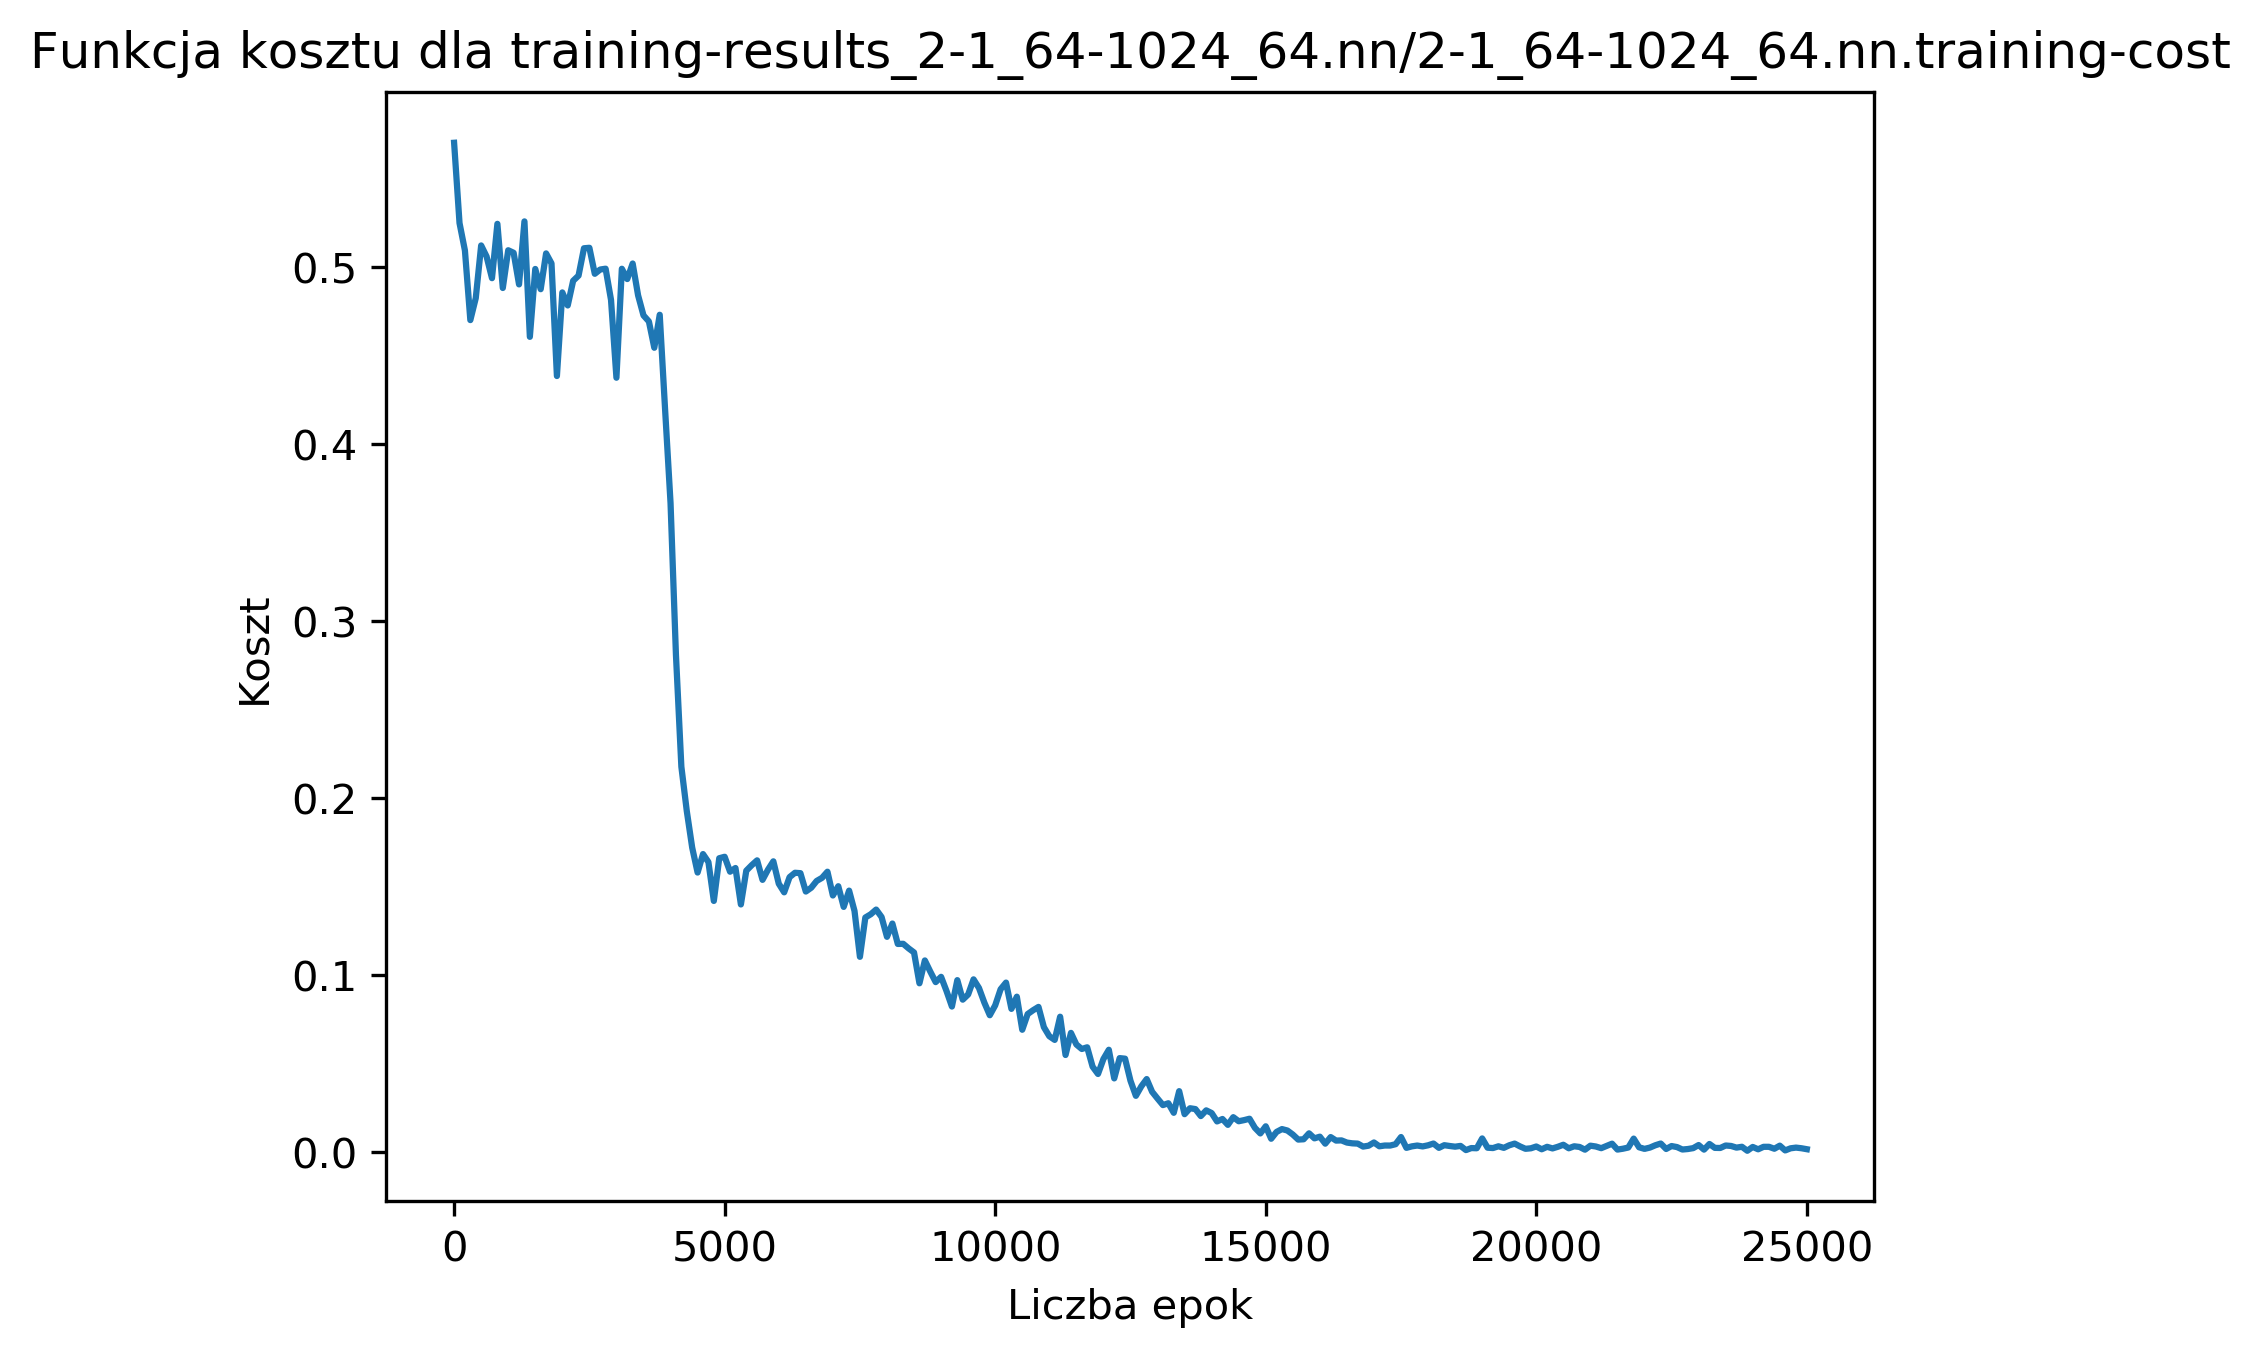
\includegraphics[width=120mm]{wykresy/2-1_64-1024_64_nn_training-cost.png}
            \end{figure}
            \begin{figure}[!htbp]
                \centering
                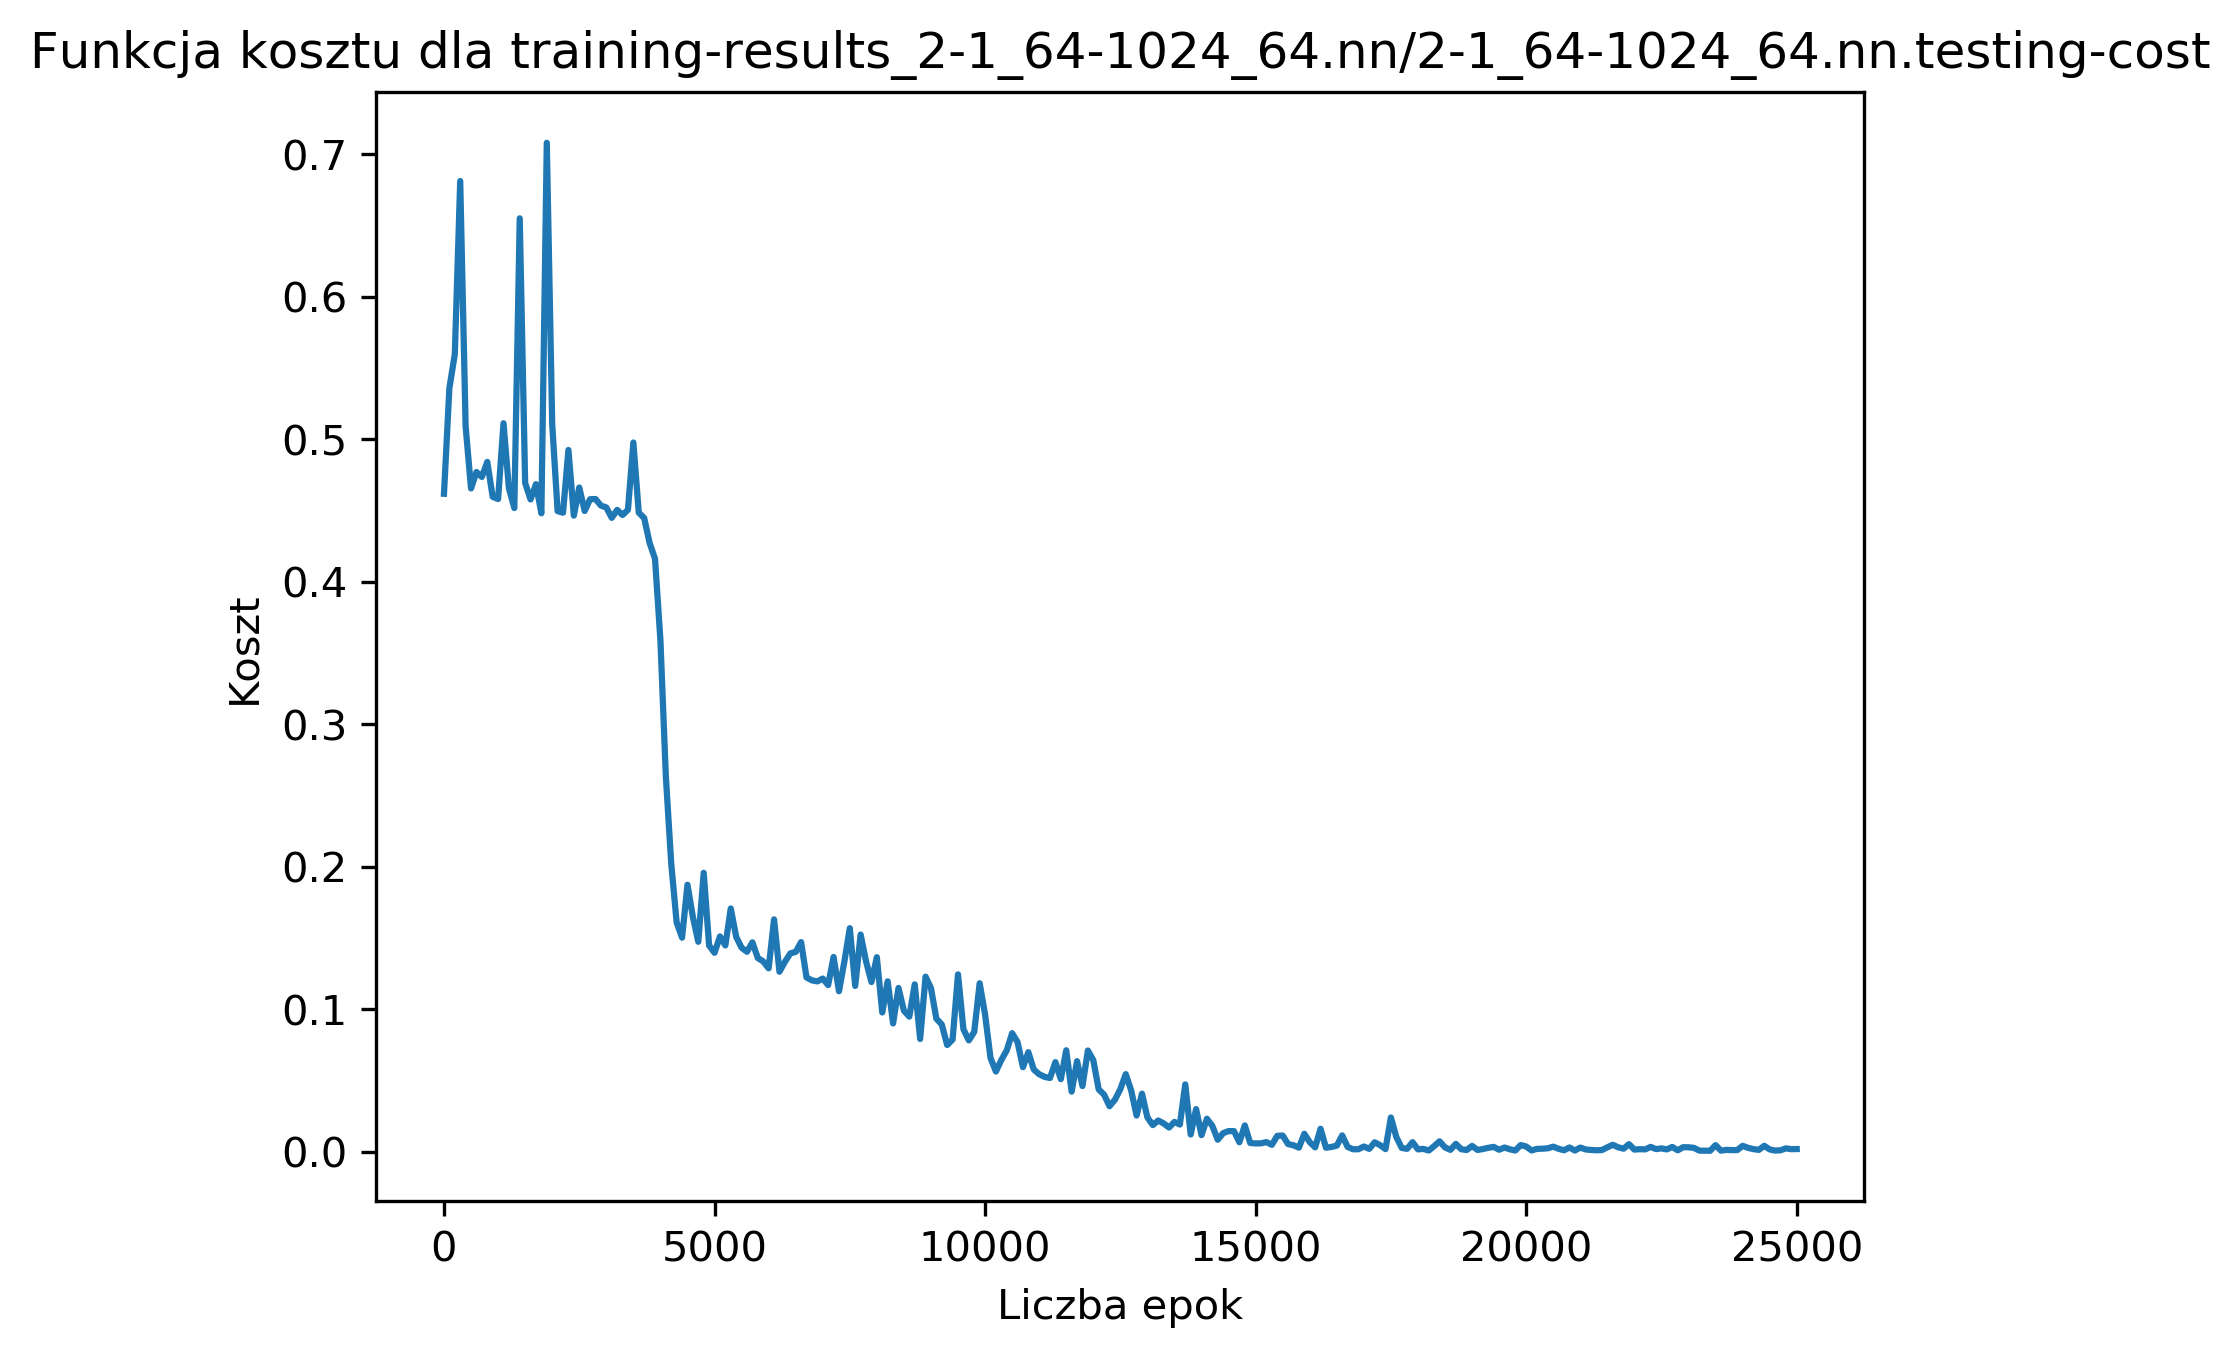
\includegraphics[width=120mm]{wykresy/2-1_64-1024_64_nn_testing-cost.png}
            \end{figure}
            \begin{figure}[!htbp]
                \centering
                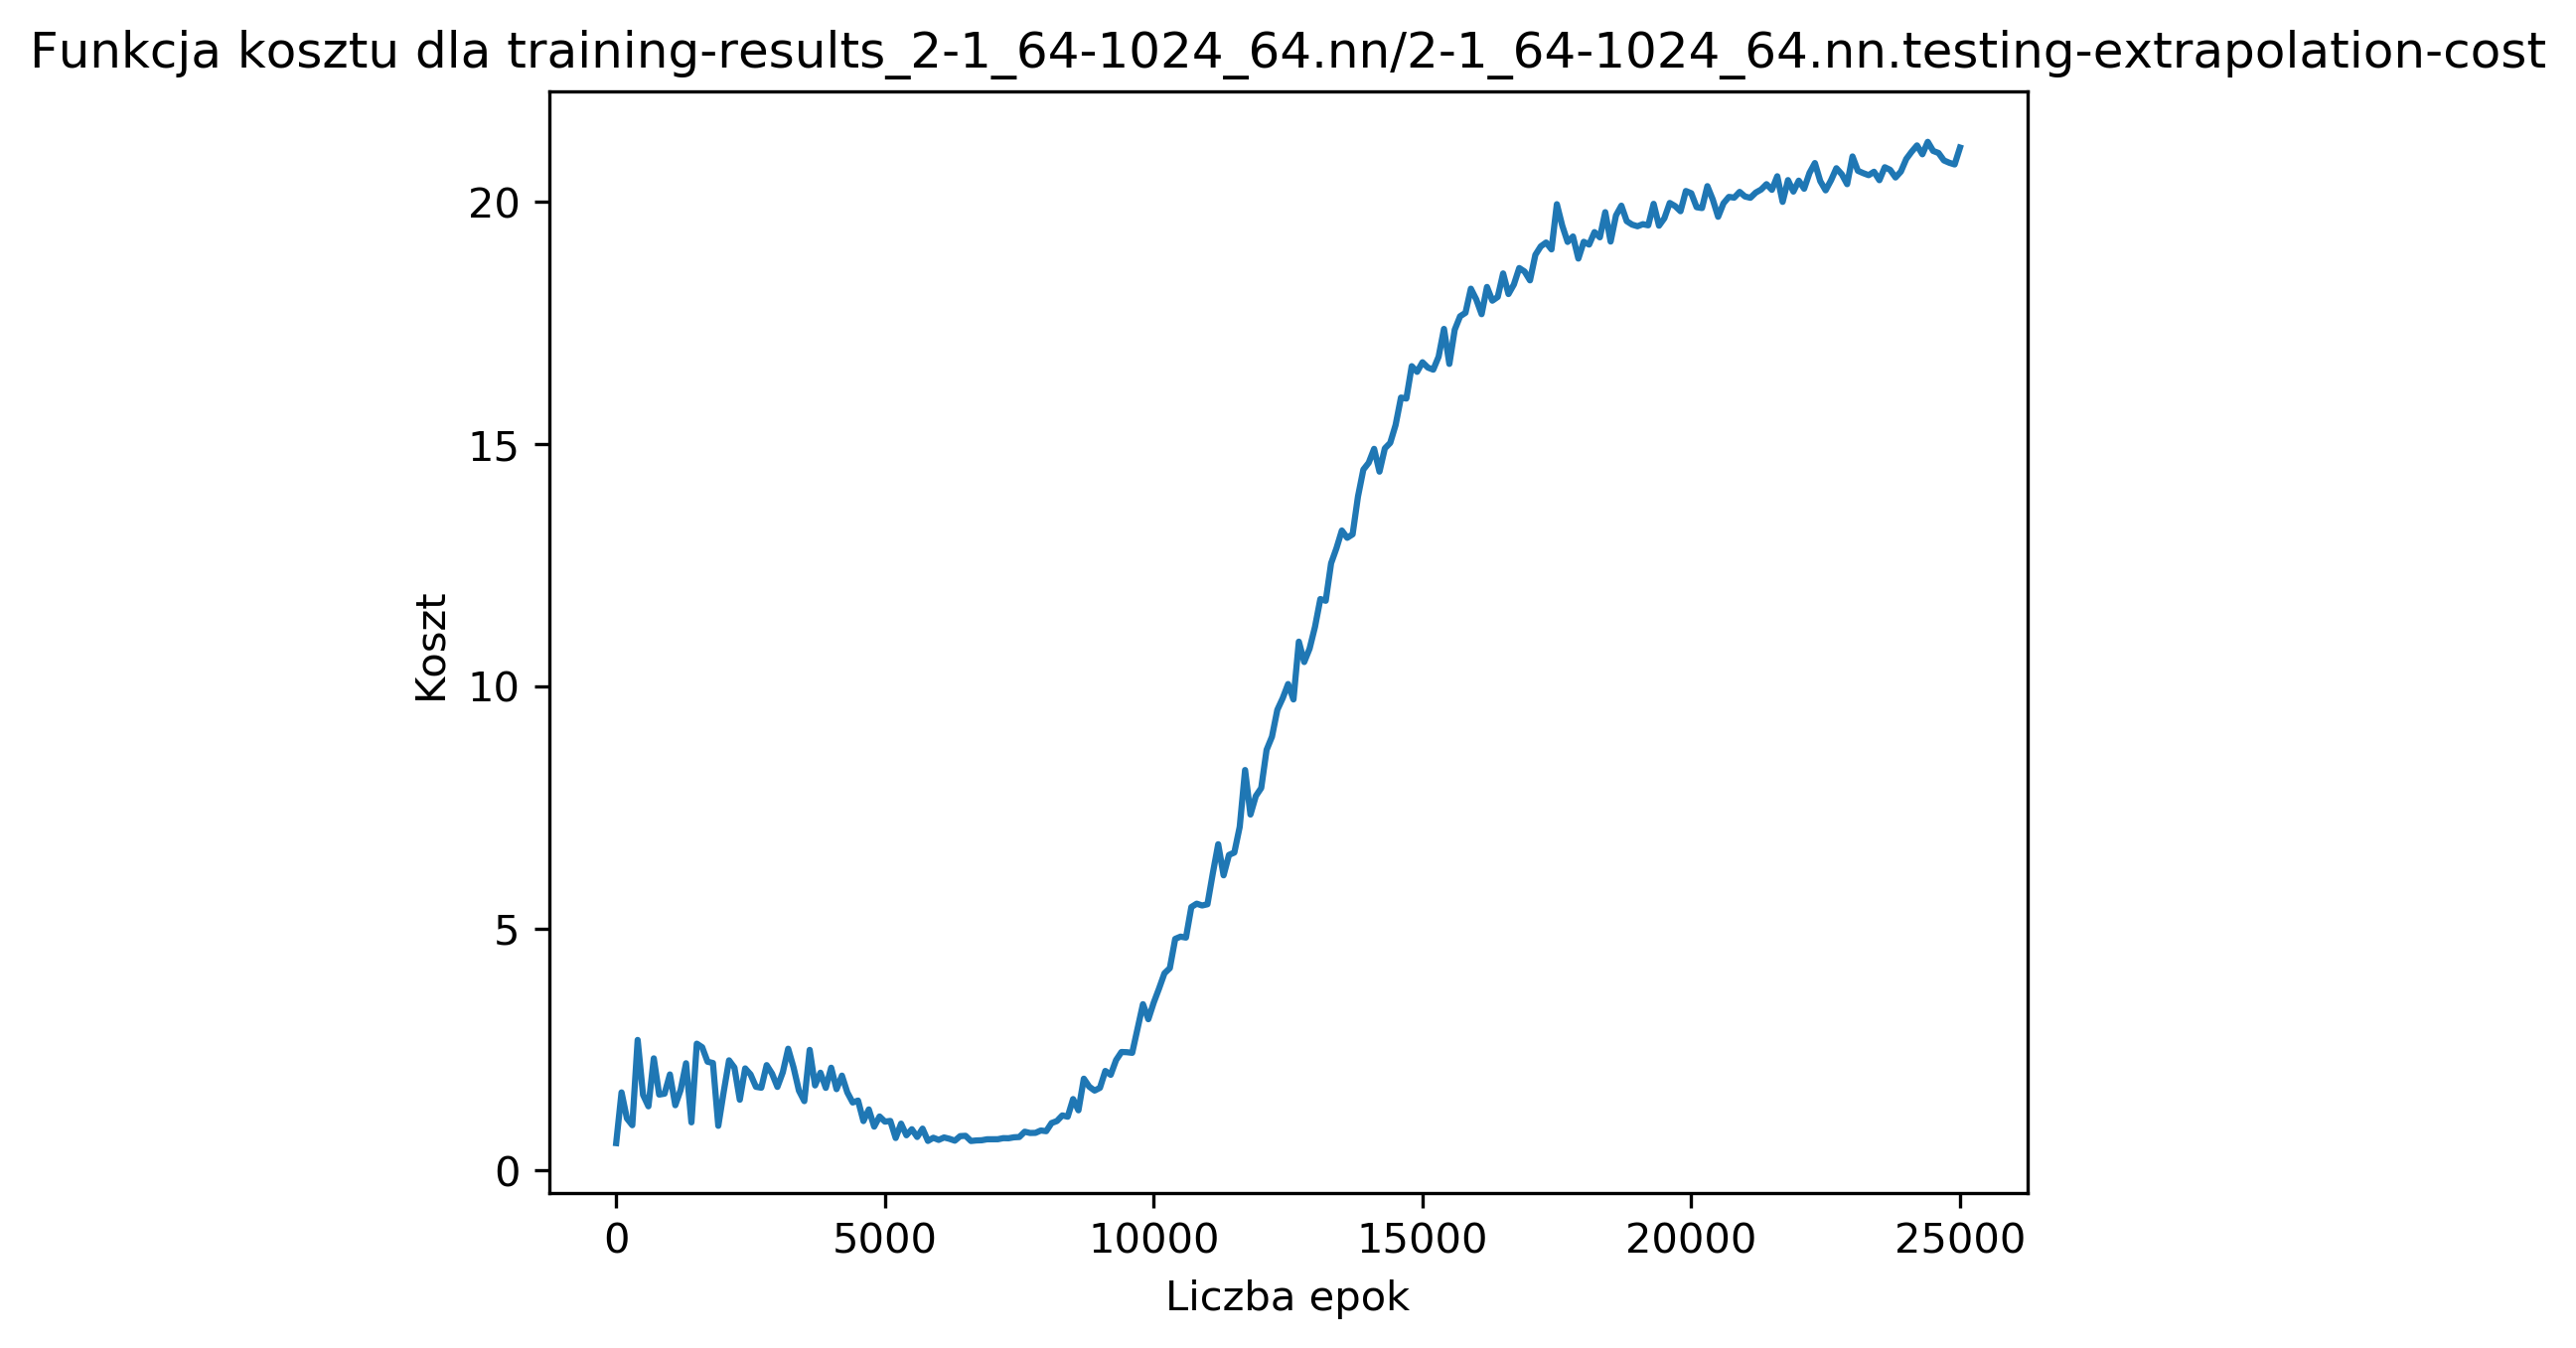
\includegraphics[width=140mm]{wykresy/2-1_64-1024_64_nn_testing-extrapolation-cost.png}
            \end{figure}
            \FloatBarrier
        %---------------------------------------------------%
            \begin{figure}[!htbp]
                \centering
                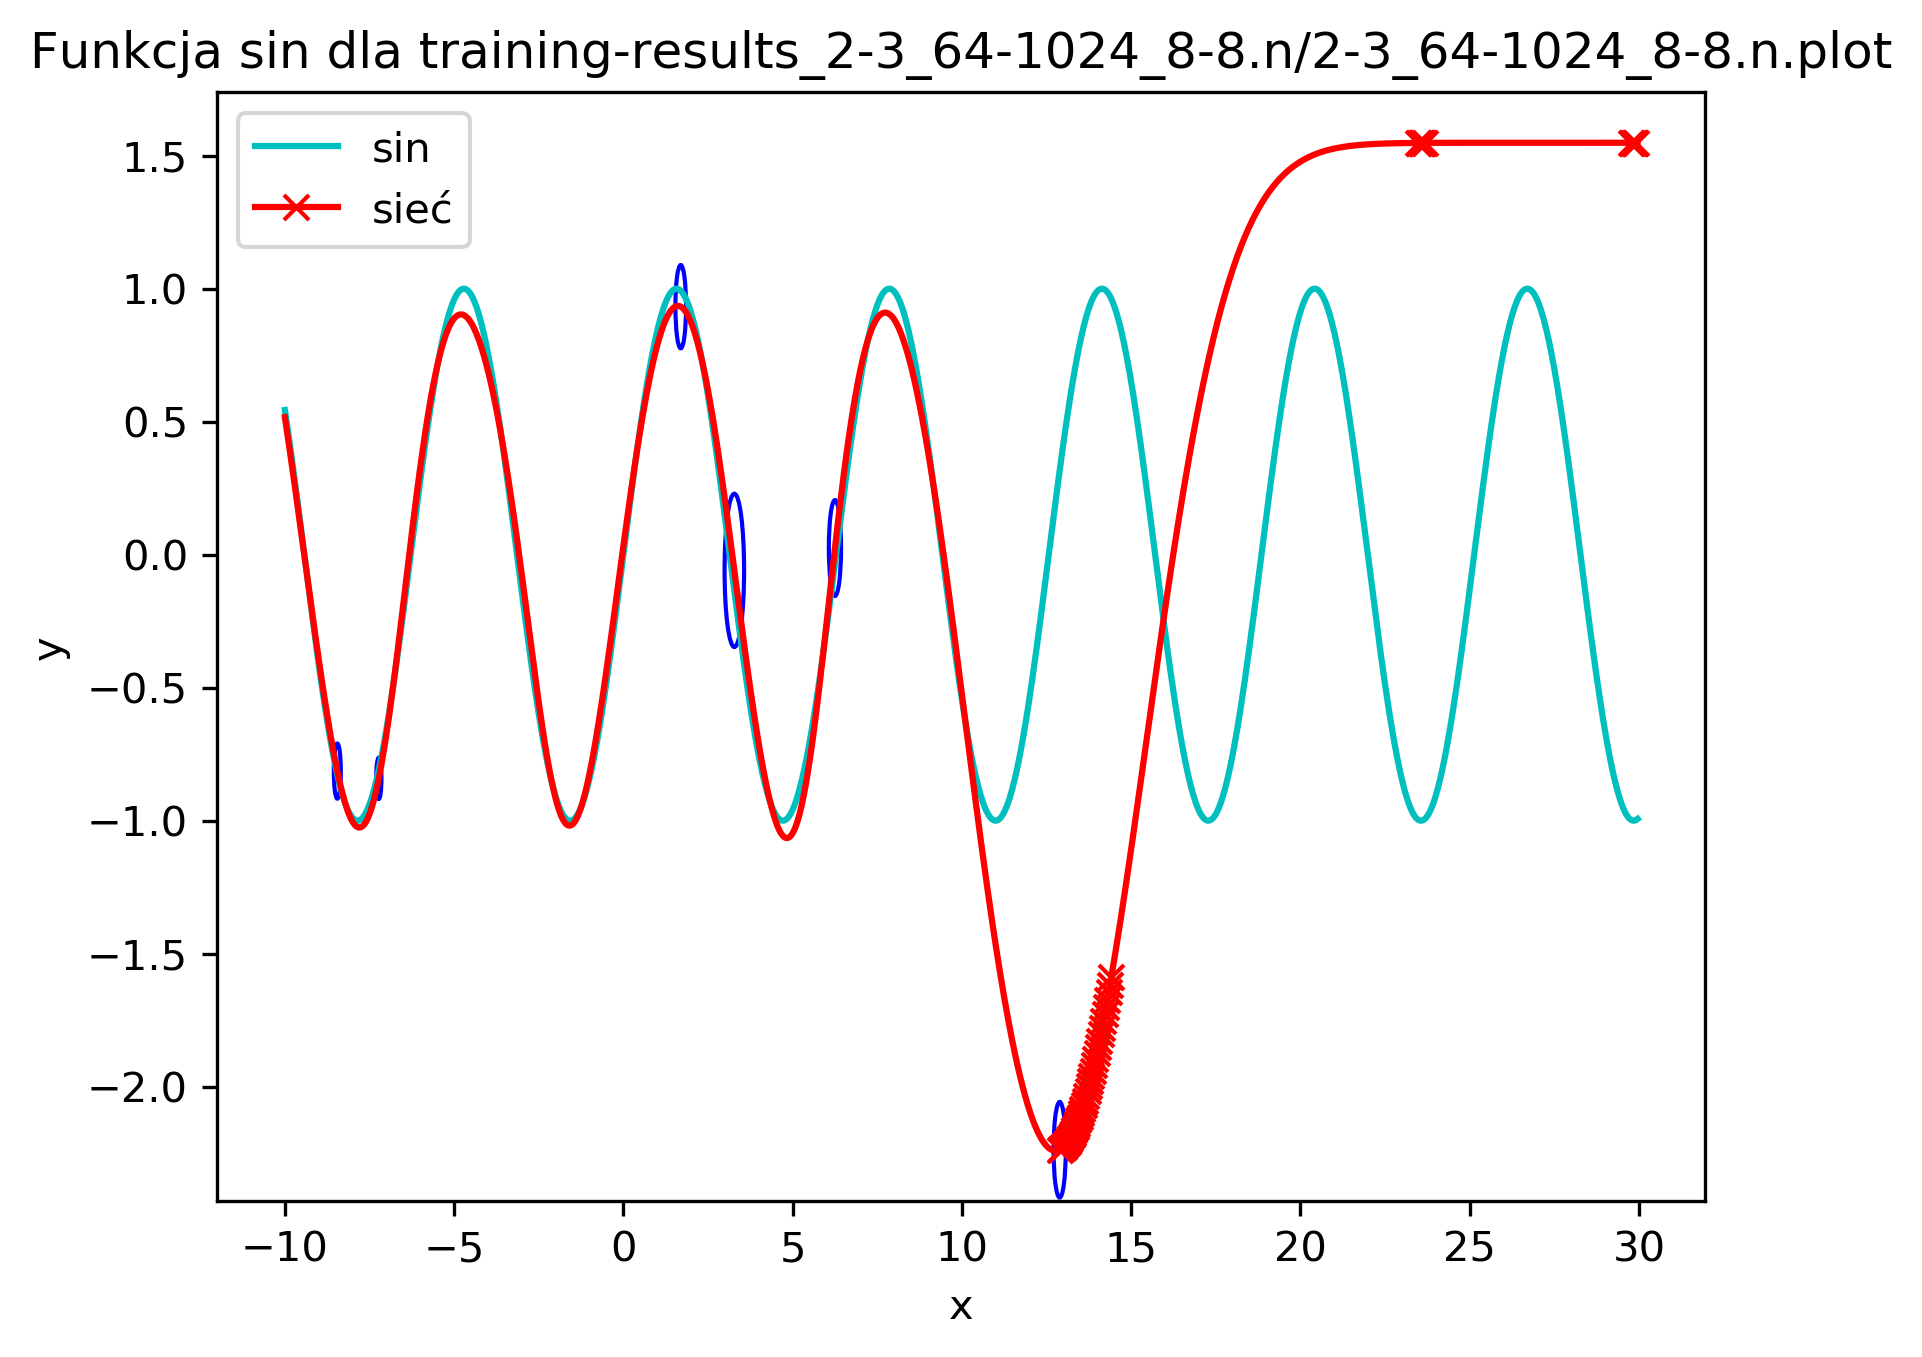
\includegraphics[width=105mm]{wykresy/2-3_64-1024_8-8_n_plot.png}
            \end{figure}
            \begin{figure}[!htbp]
                \centering
                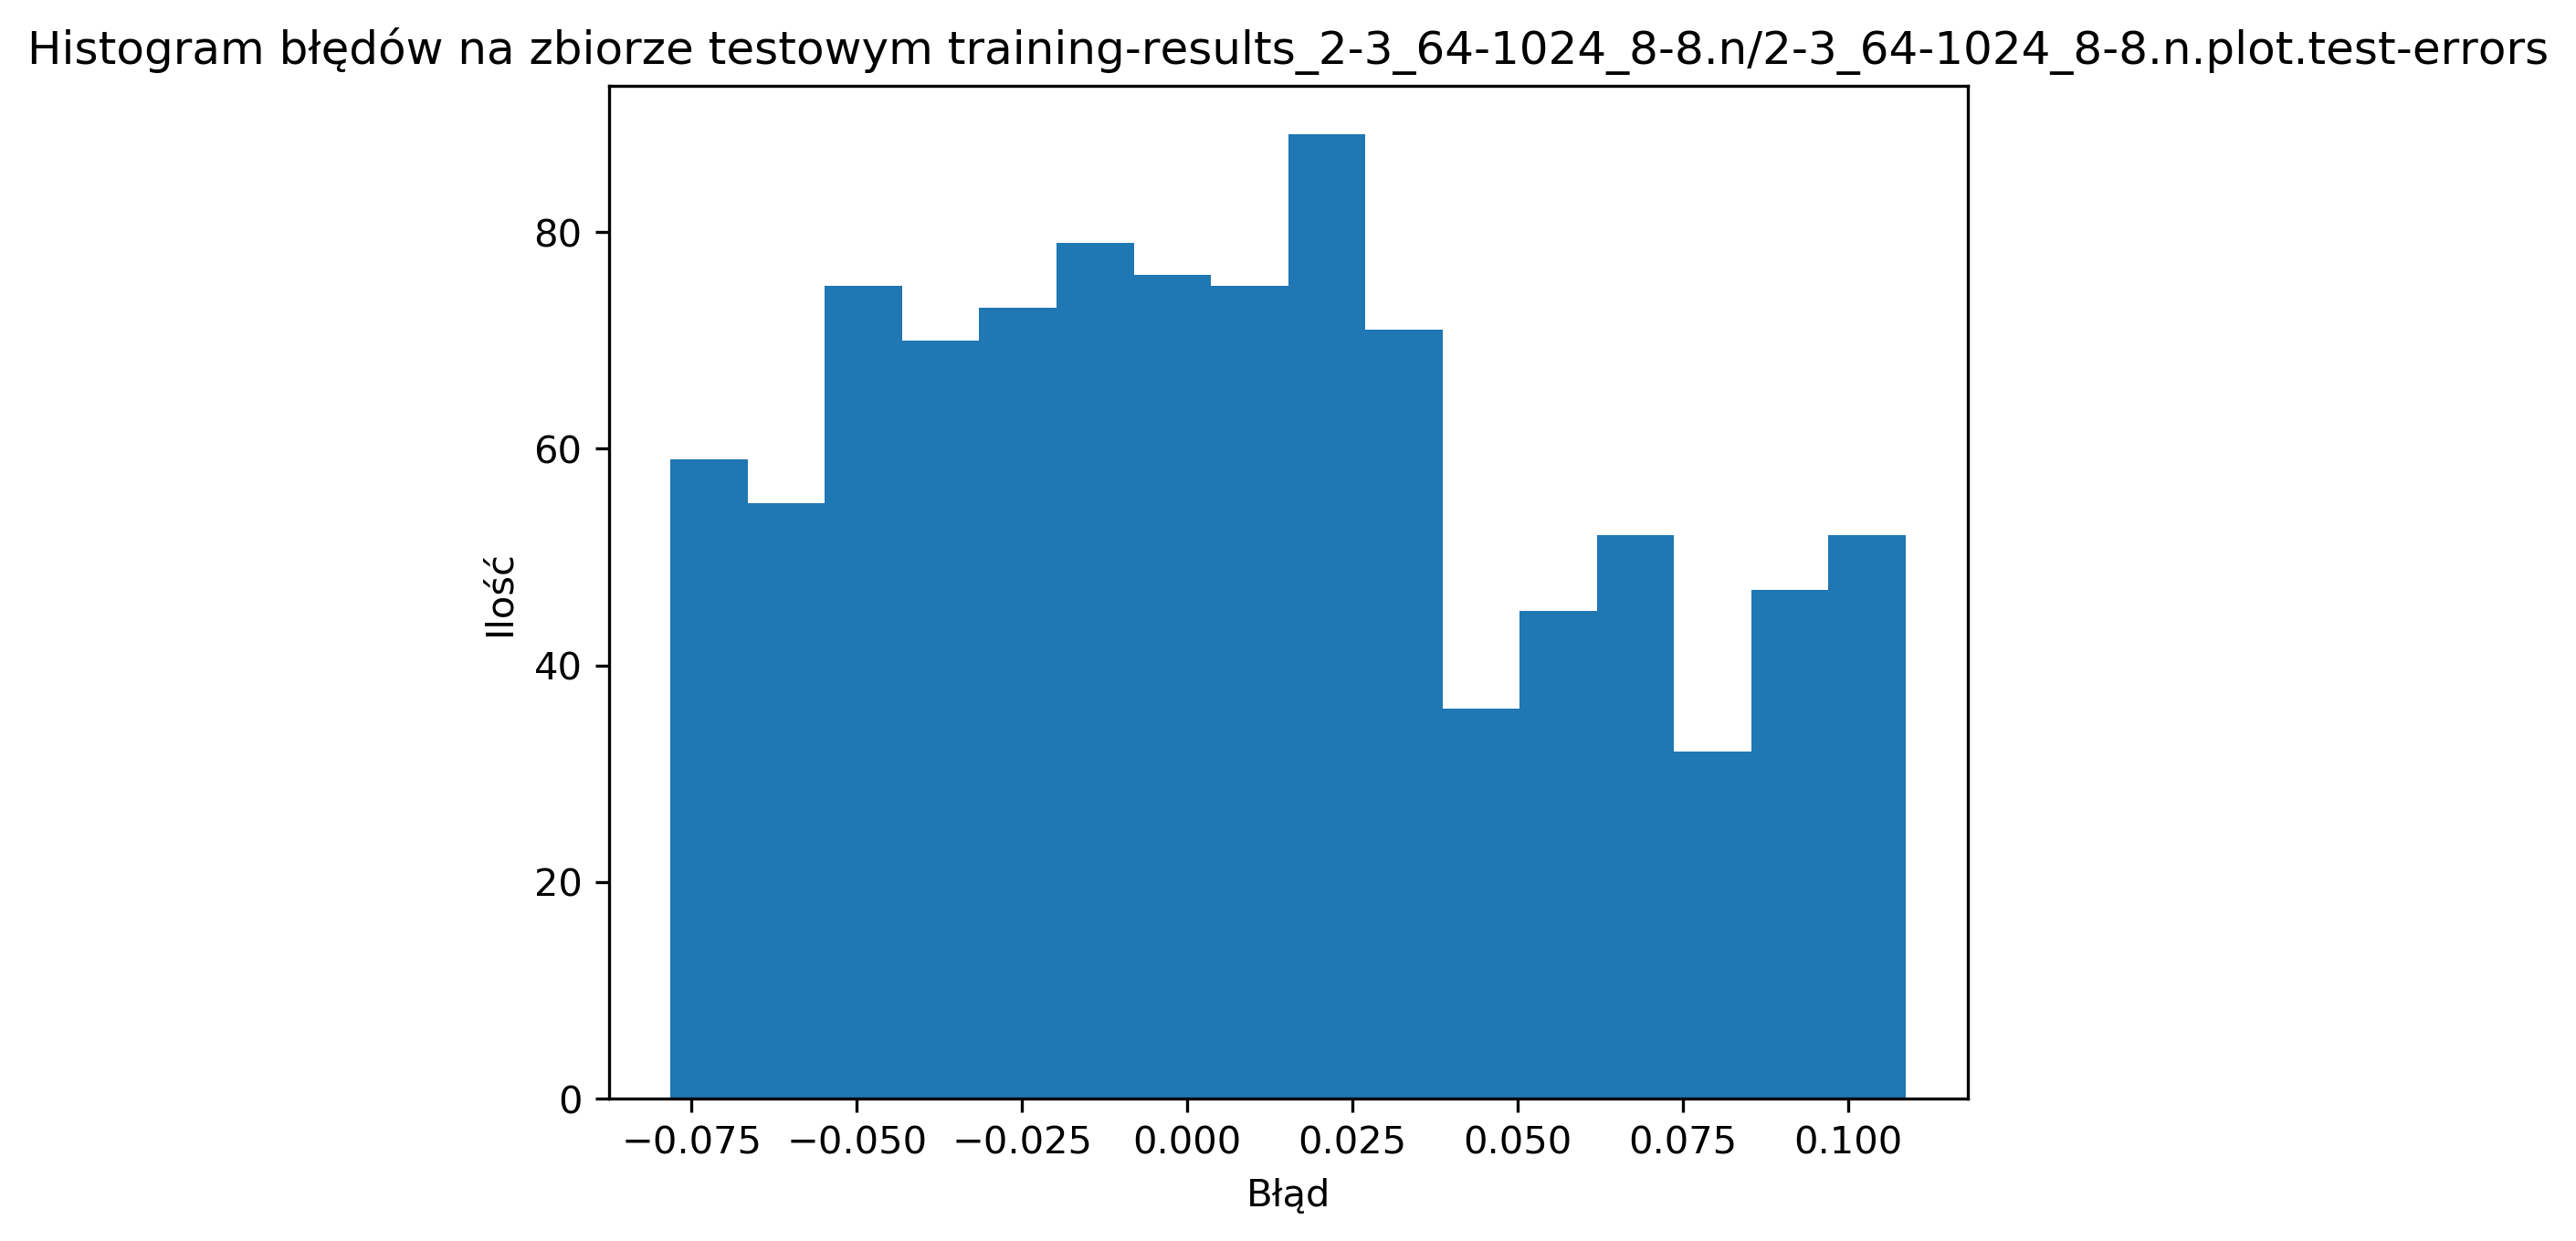
\includegraphics[width=140mm]{wykresy/2-3_64-1024_8-8_n_plot_test-errors.png}
            \end{figure}
            \begin{figure}[!htbp]
                \centering
                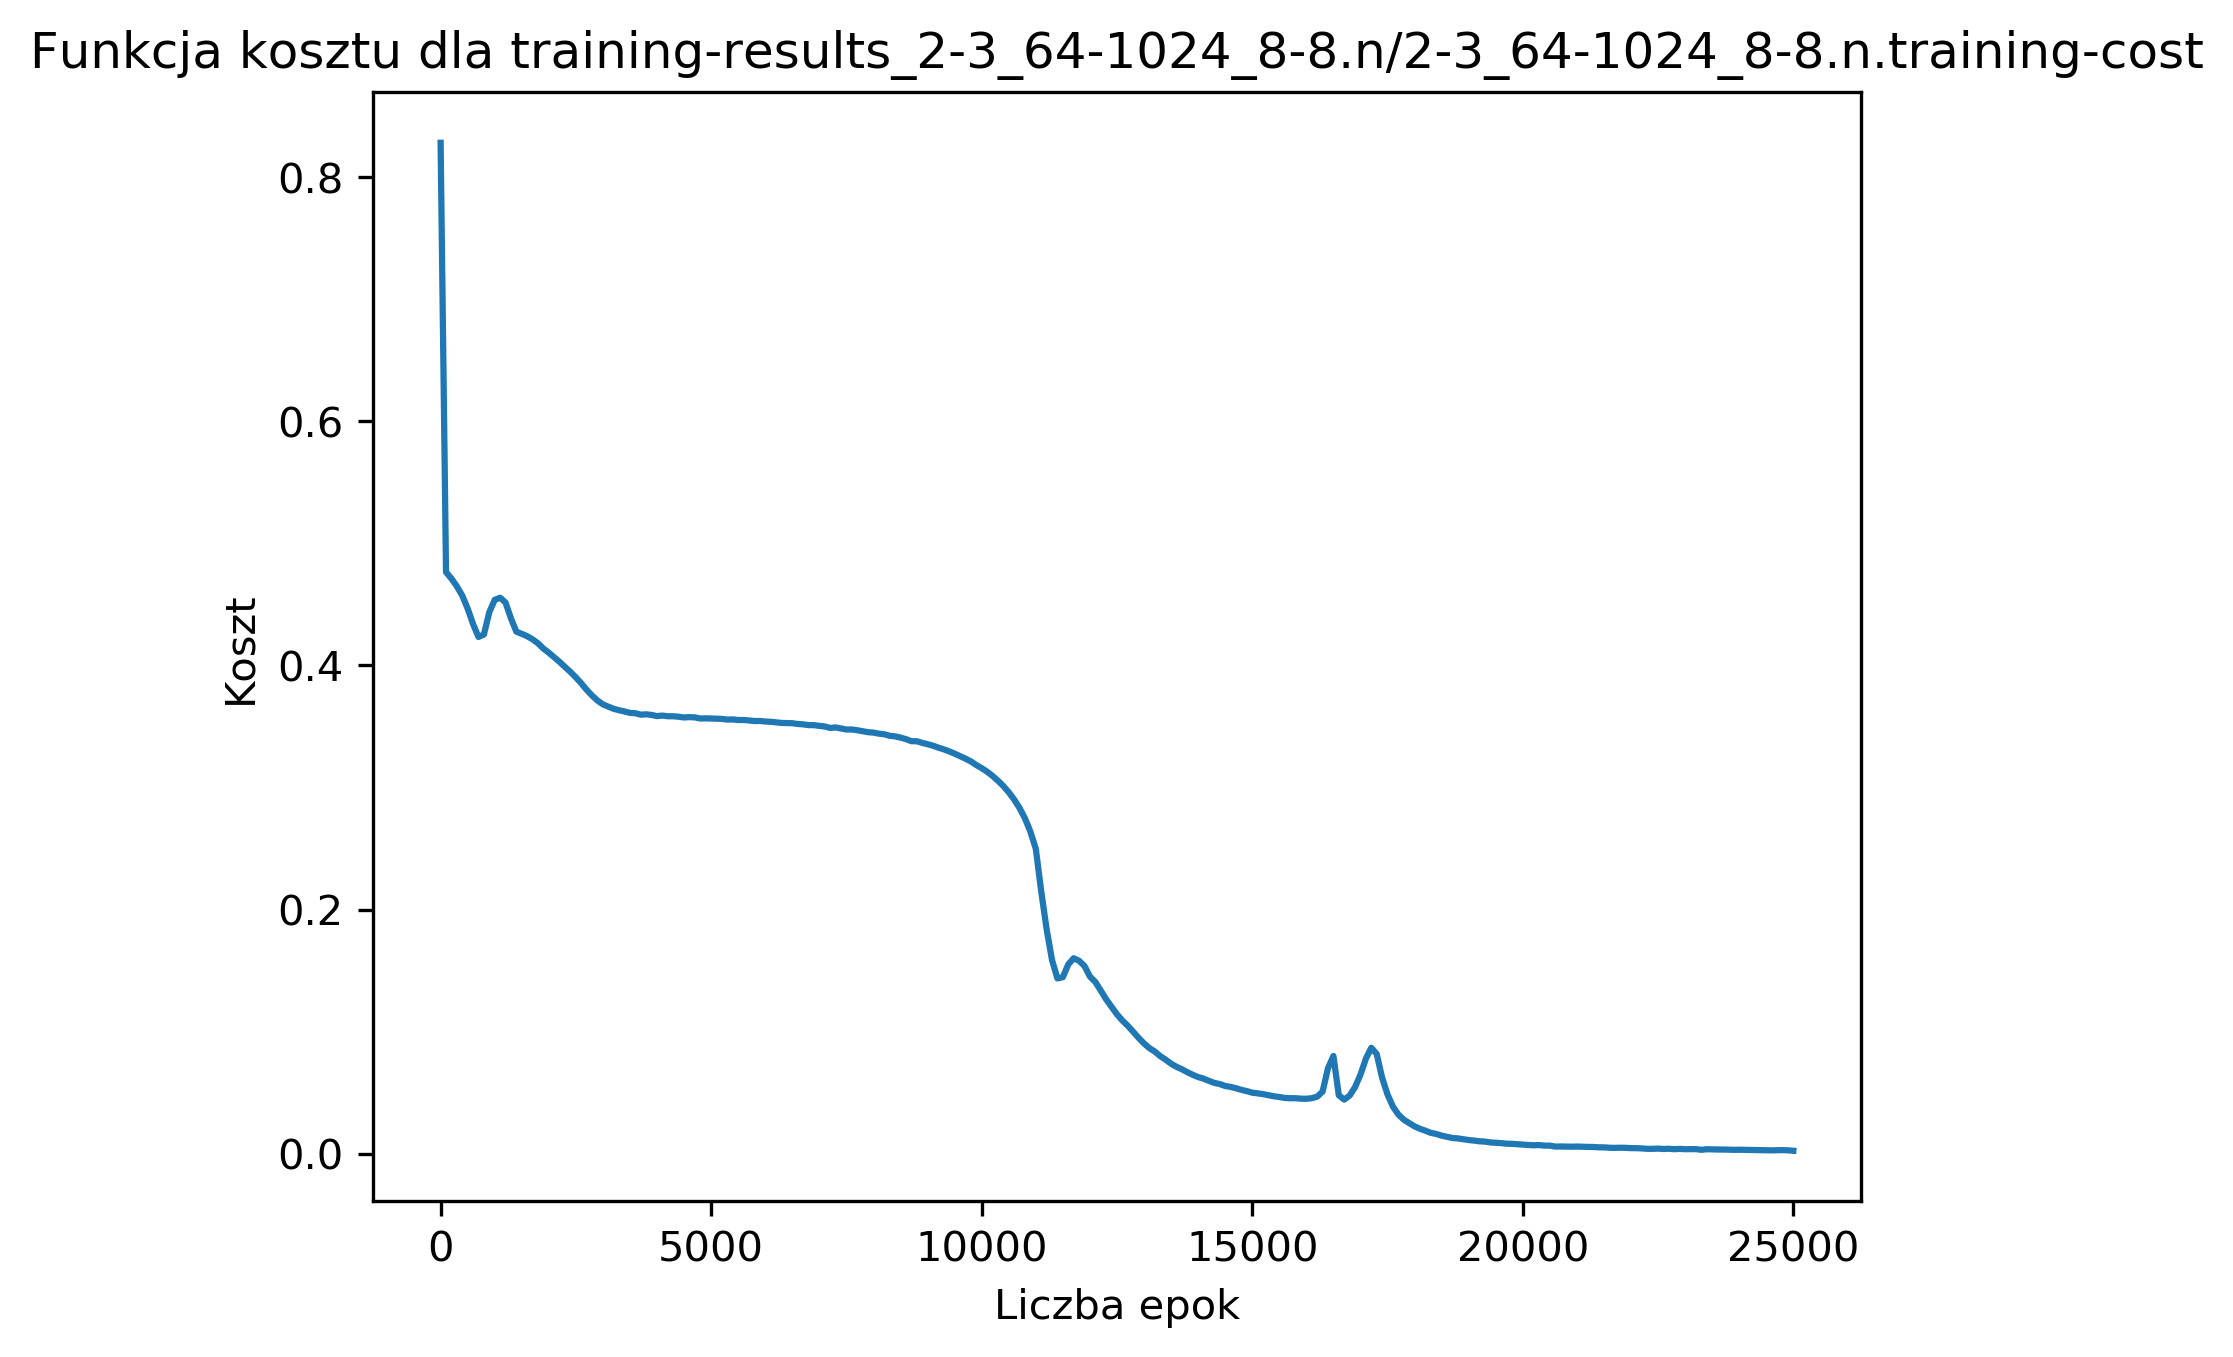
\includegraphics[width=120mm]{wykresy/2-3_64-1024_8-8_n_training-cost.png}
            \end{figure}
            \begin{figure}[!htbp]
                \centering
                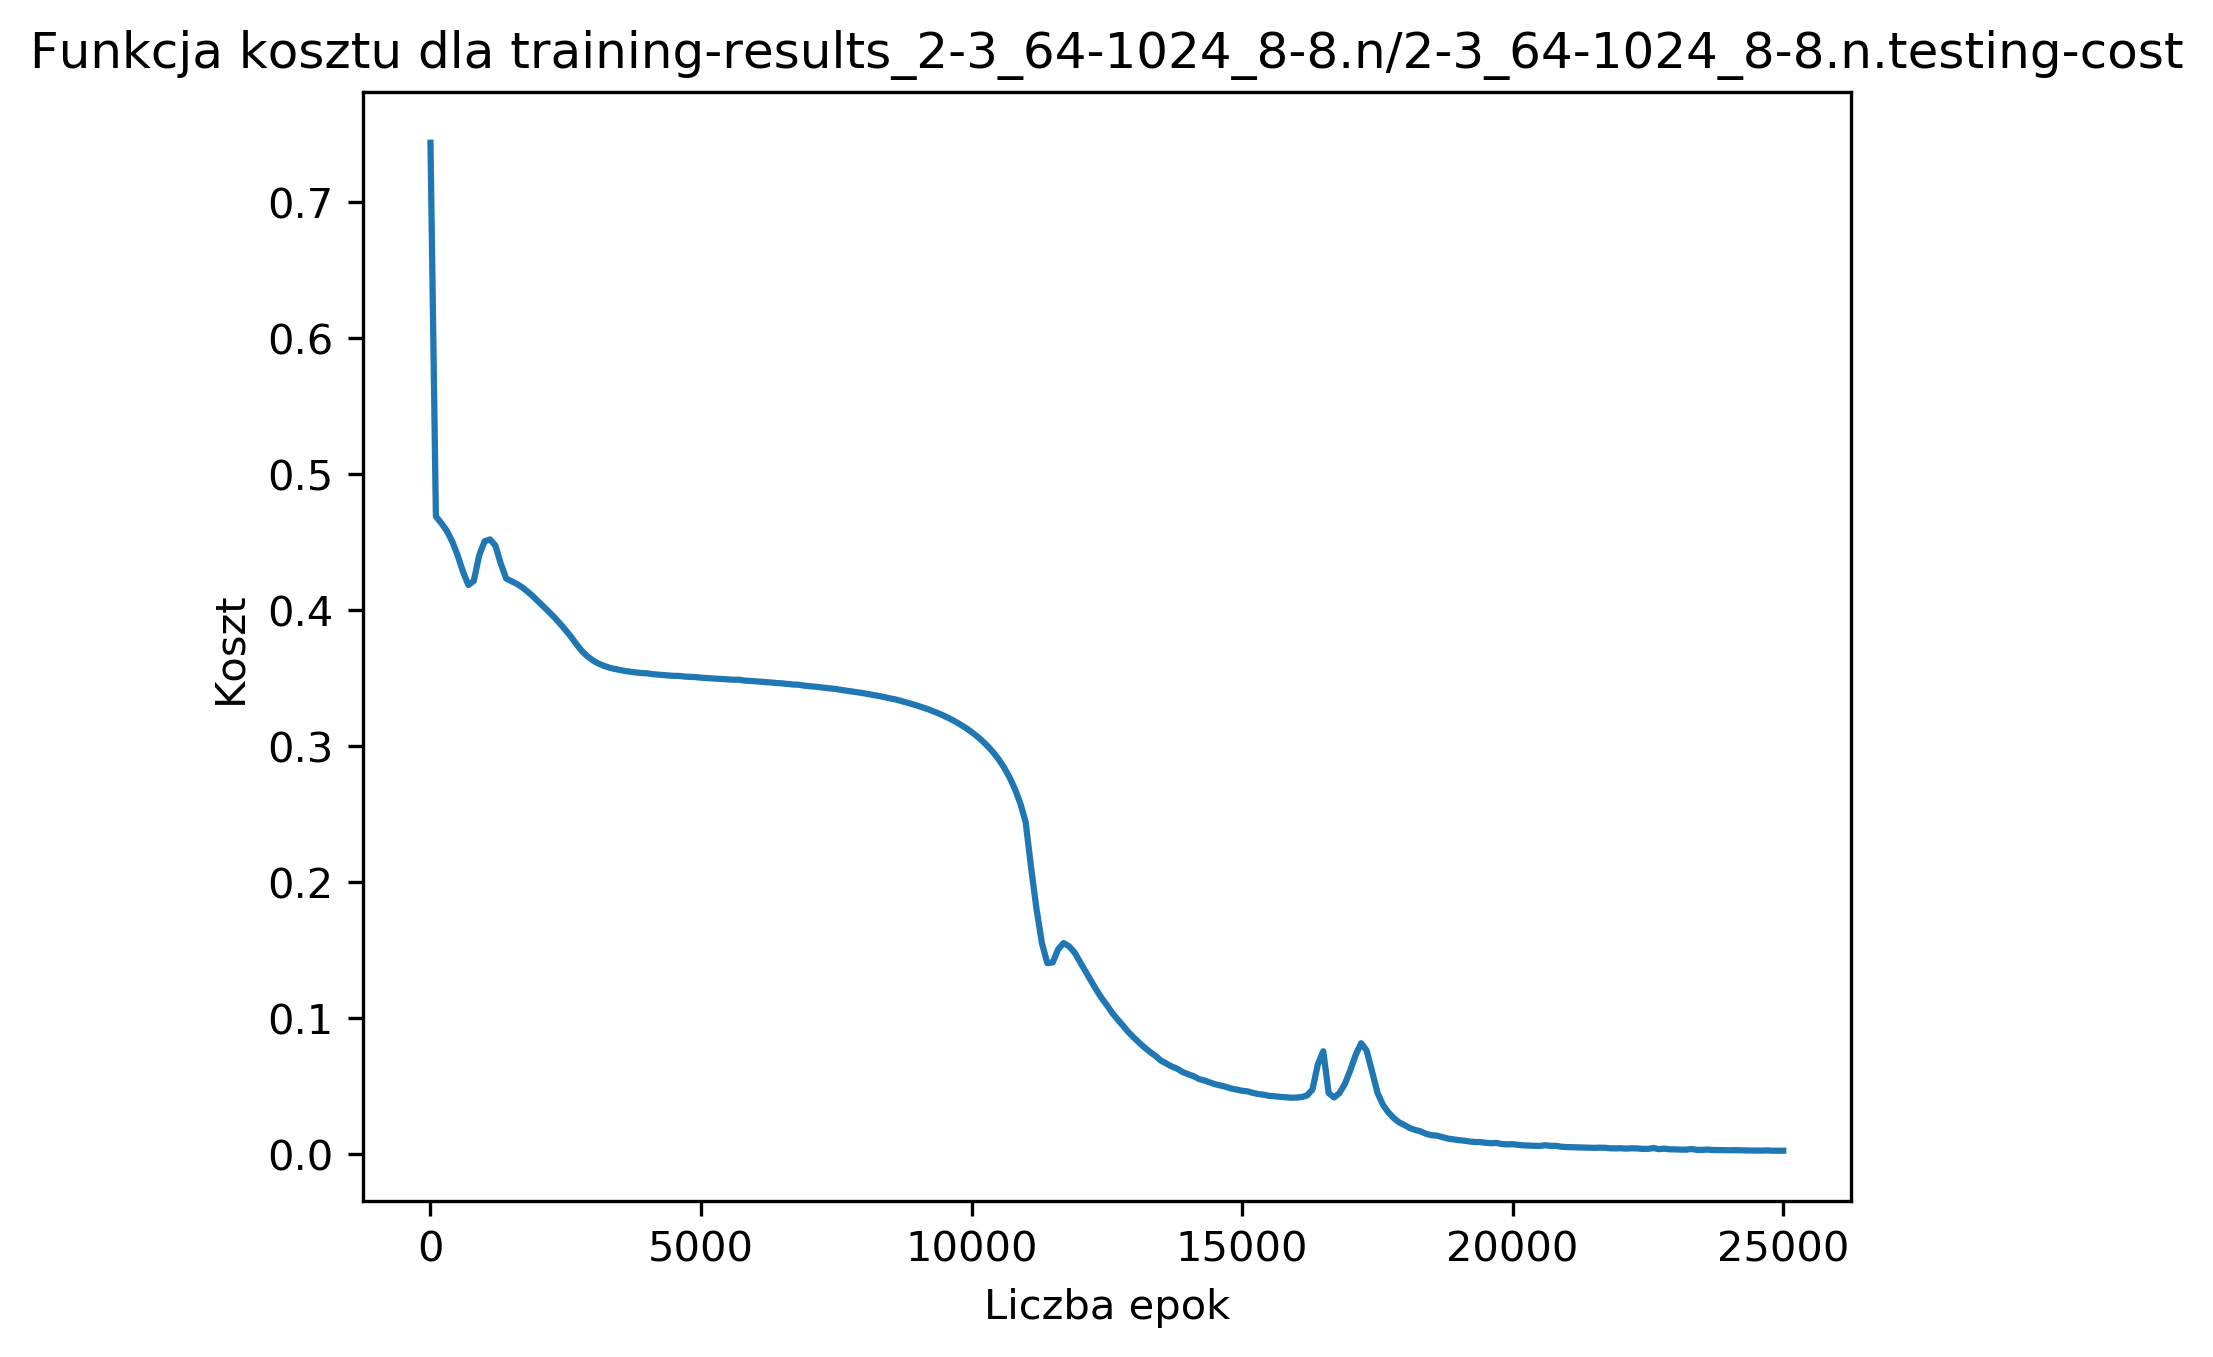
\includegraphics[width=120mm]{wykresy/2-3_64-1024_8-8_n_testing-cost.png}
            \end{figure}
            \begin{figure}[!htbp]
                \centering
                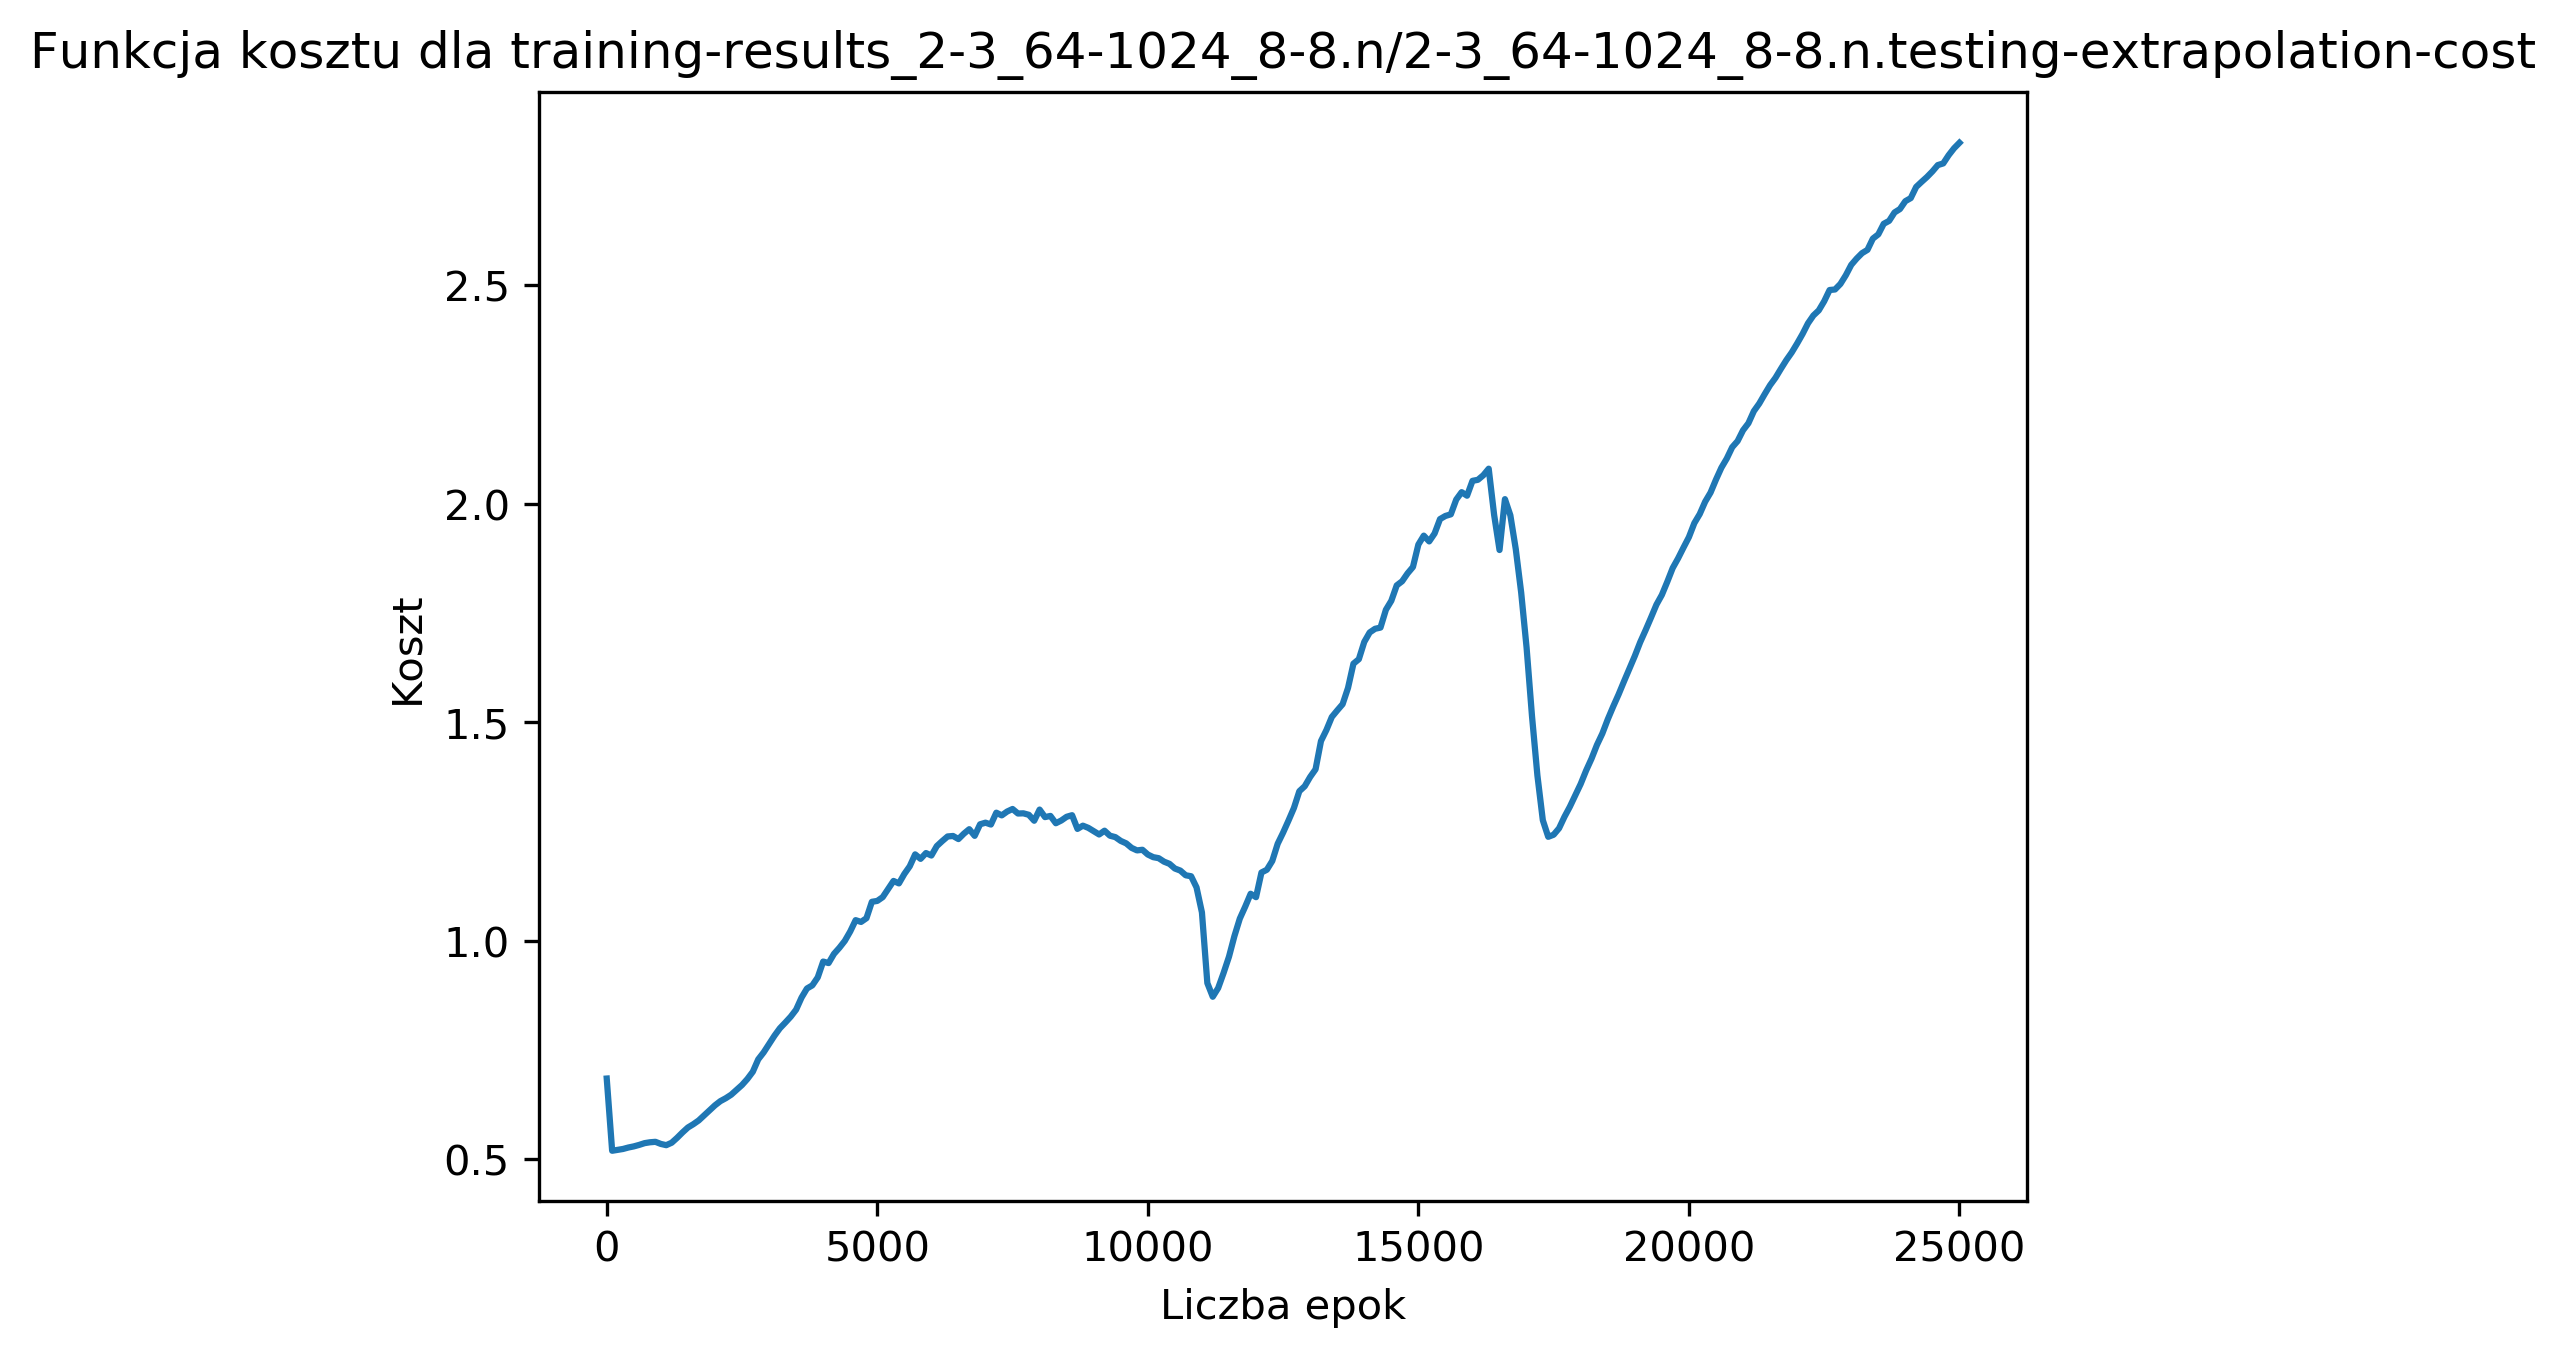
\includegraphics[width=140mm]{wykresy/2-3_64-1024_8-8_n_testing-extrapolation-cost.png}
            \end{figure}
            \FloatBarrier
        %---------------------------------------------------%
        }
    %---------------------------------------------------%
        \subsection{Funkcja 3}
        {
            \begin{figure}[!htbp]
                \centering
                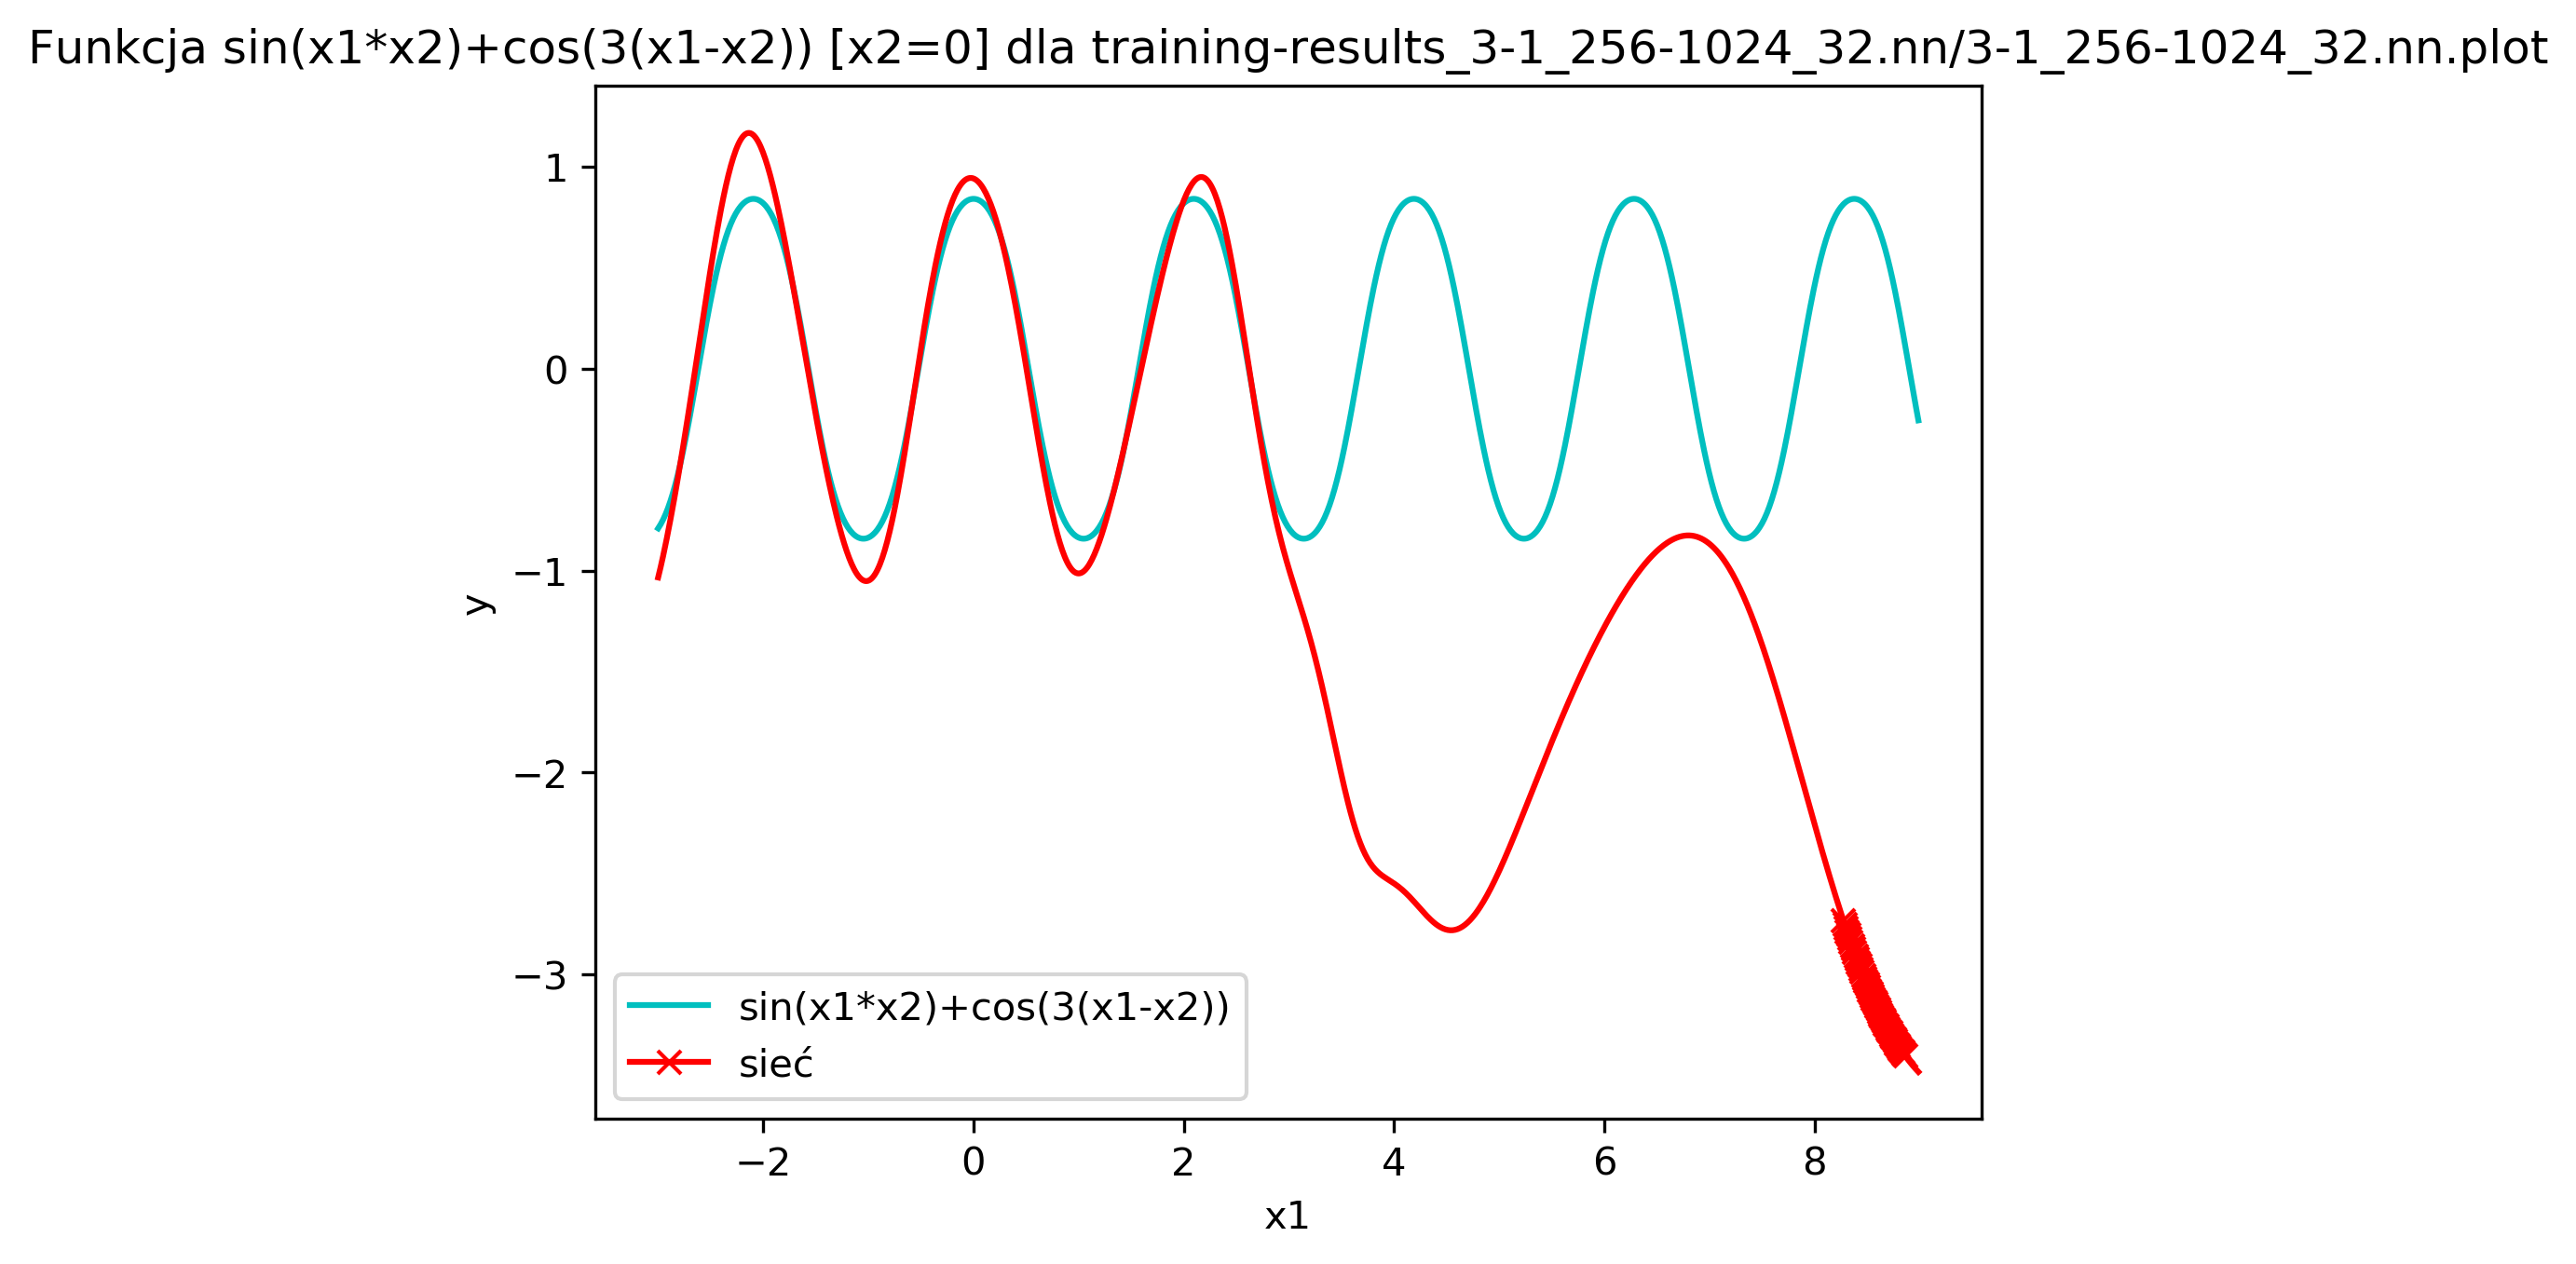
\includegraphics[width=135mm]{wykresy/3-1_256-1024_32_nn_plot1.png}
            \end{figure}
            \begin{figure}[!htbp]
                \centering
                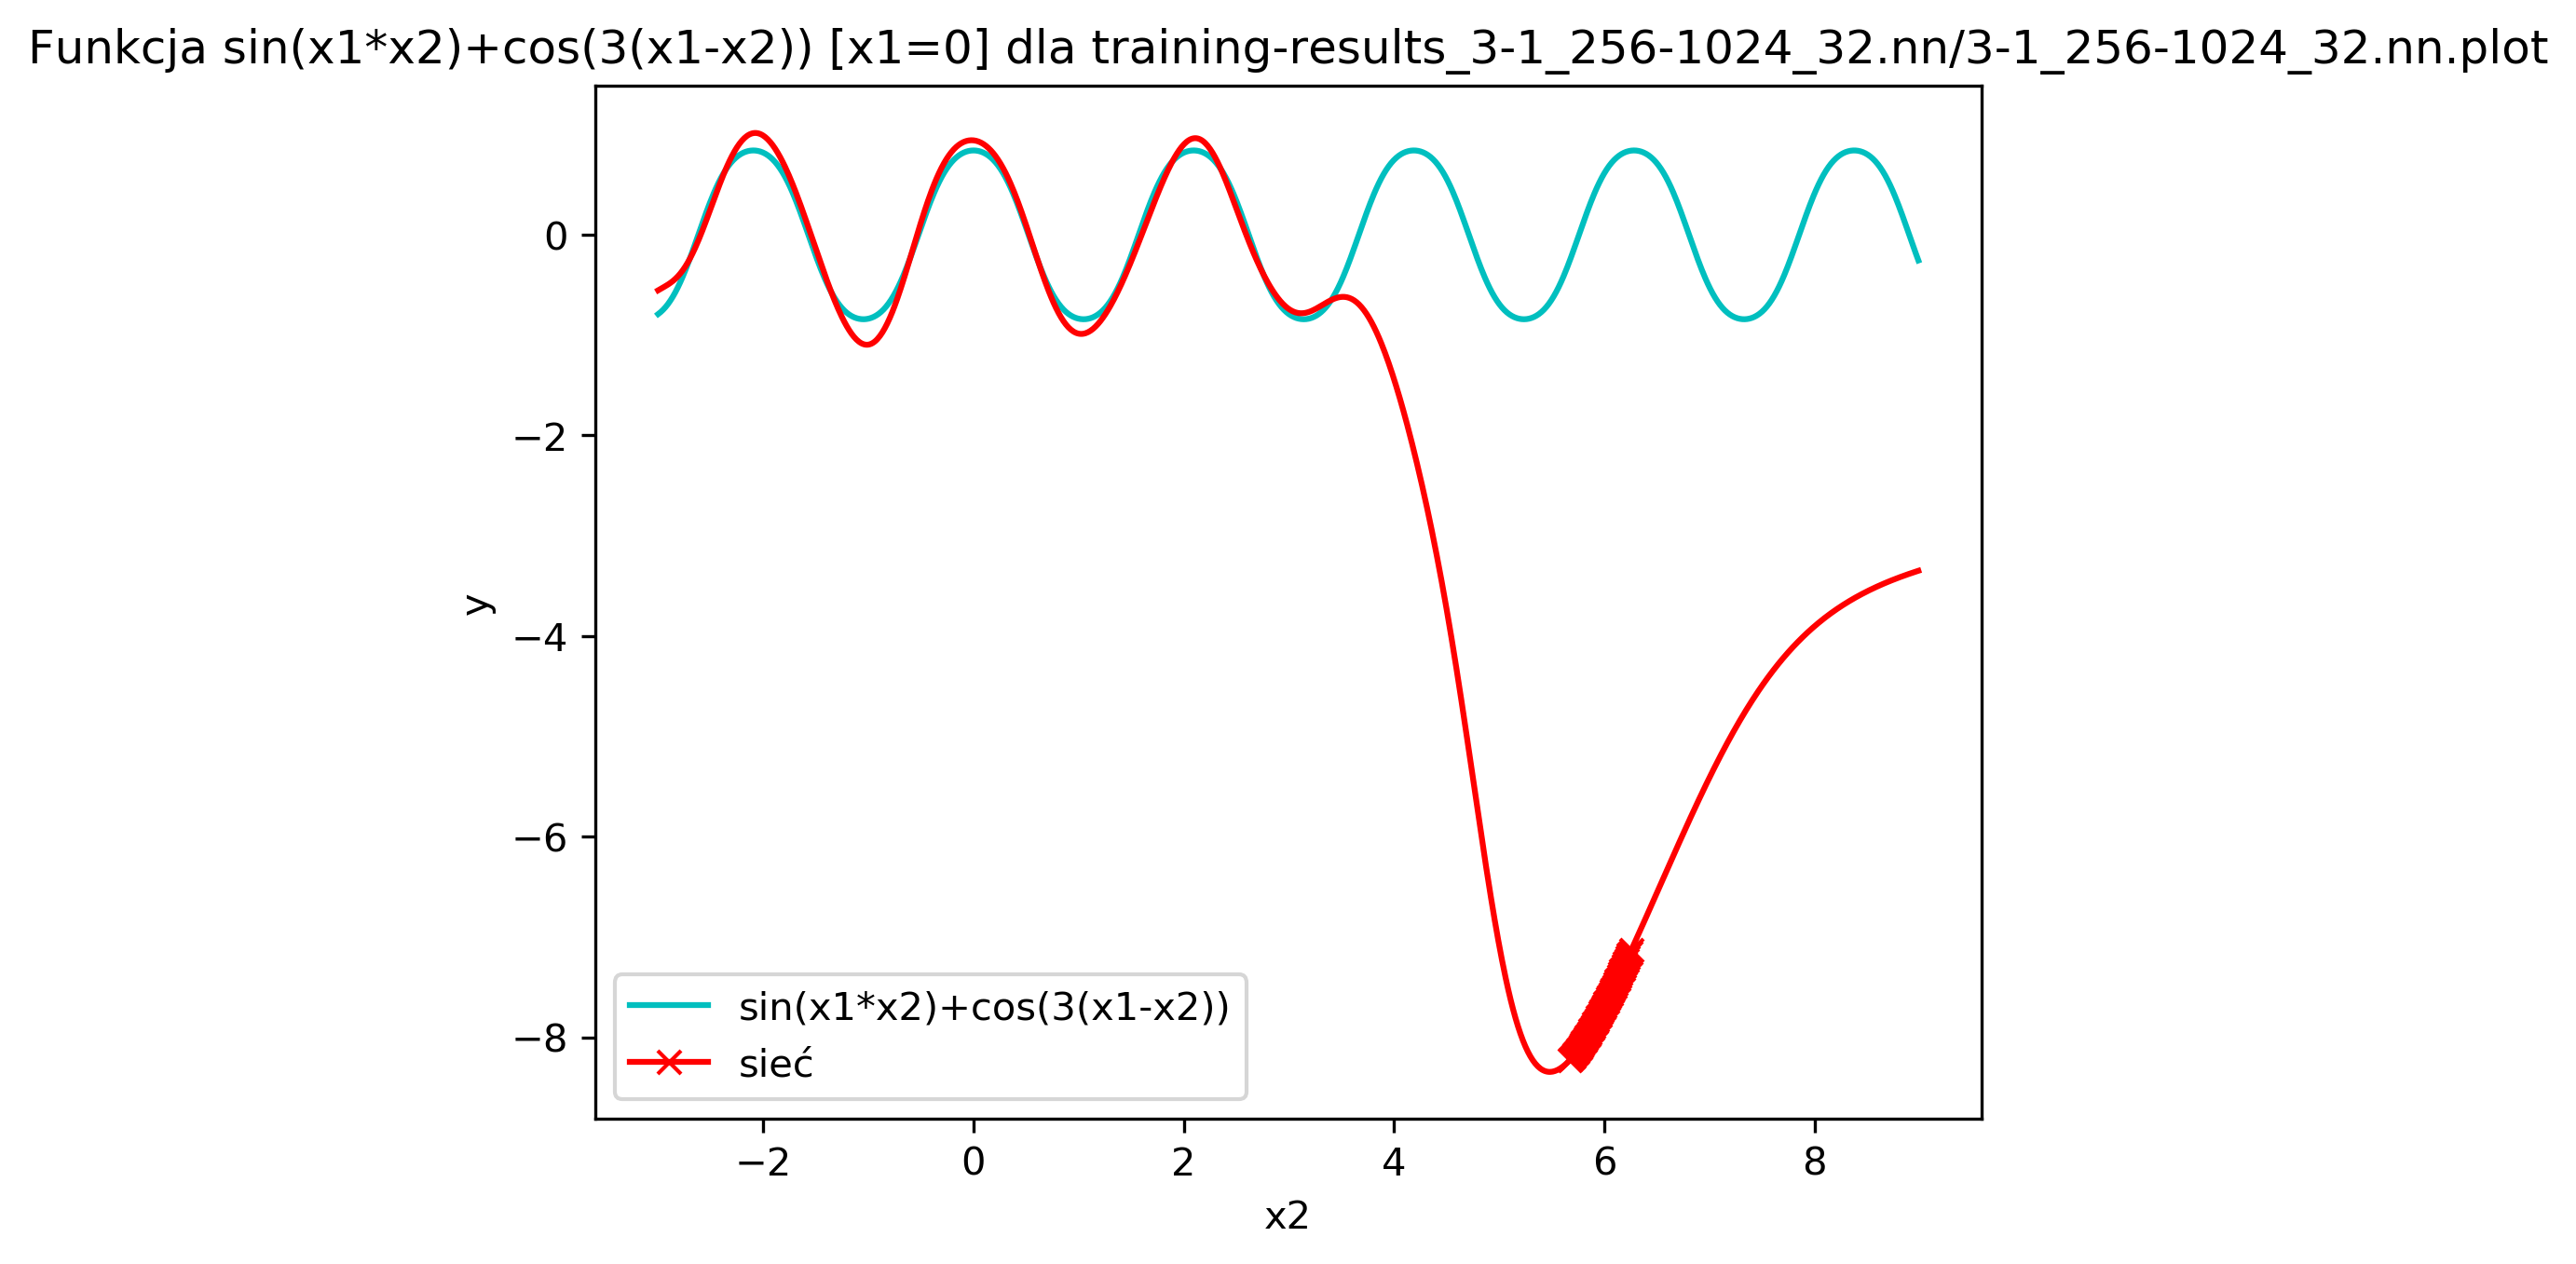
\includegraphics[width=135mm]{wykresy/3-1_256-1024_32_nn_plot2.png}
            \end{figure}
            \begin{figure}[!htbp]
                \centering
                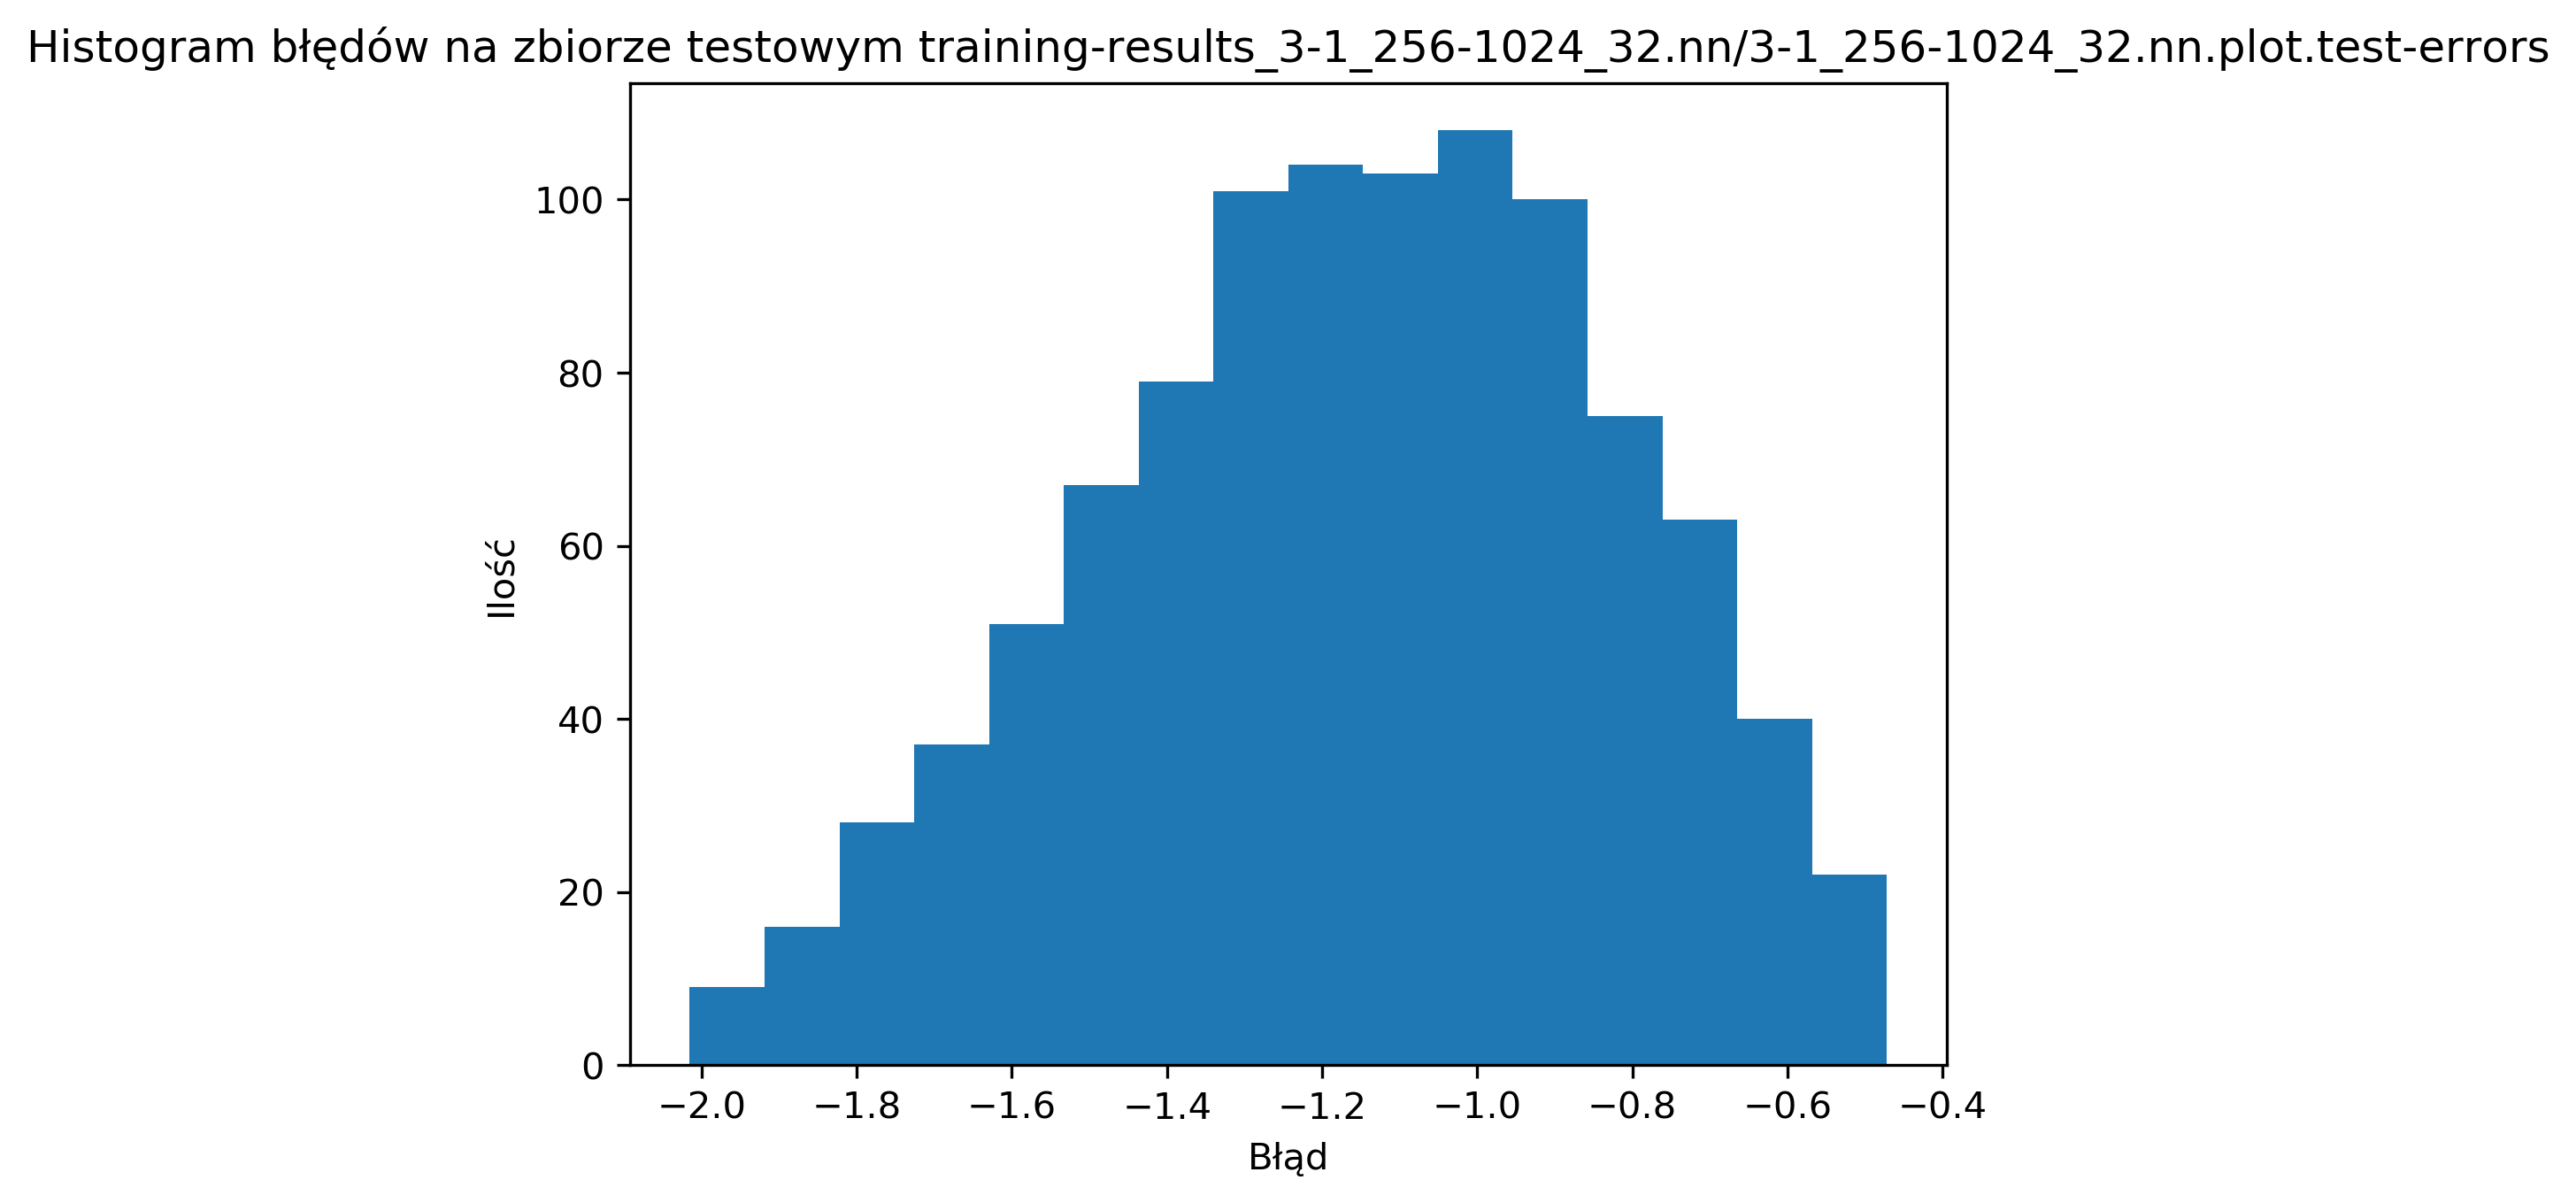
\includegraphics[width=145mm]{wykresy/3-1_256-1024_32_nn_plot_test-errors.png}
            \end{figure}
            \begin{figure}[!htbp]
                \centering
                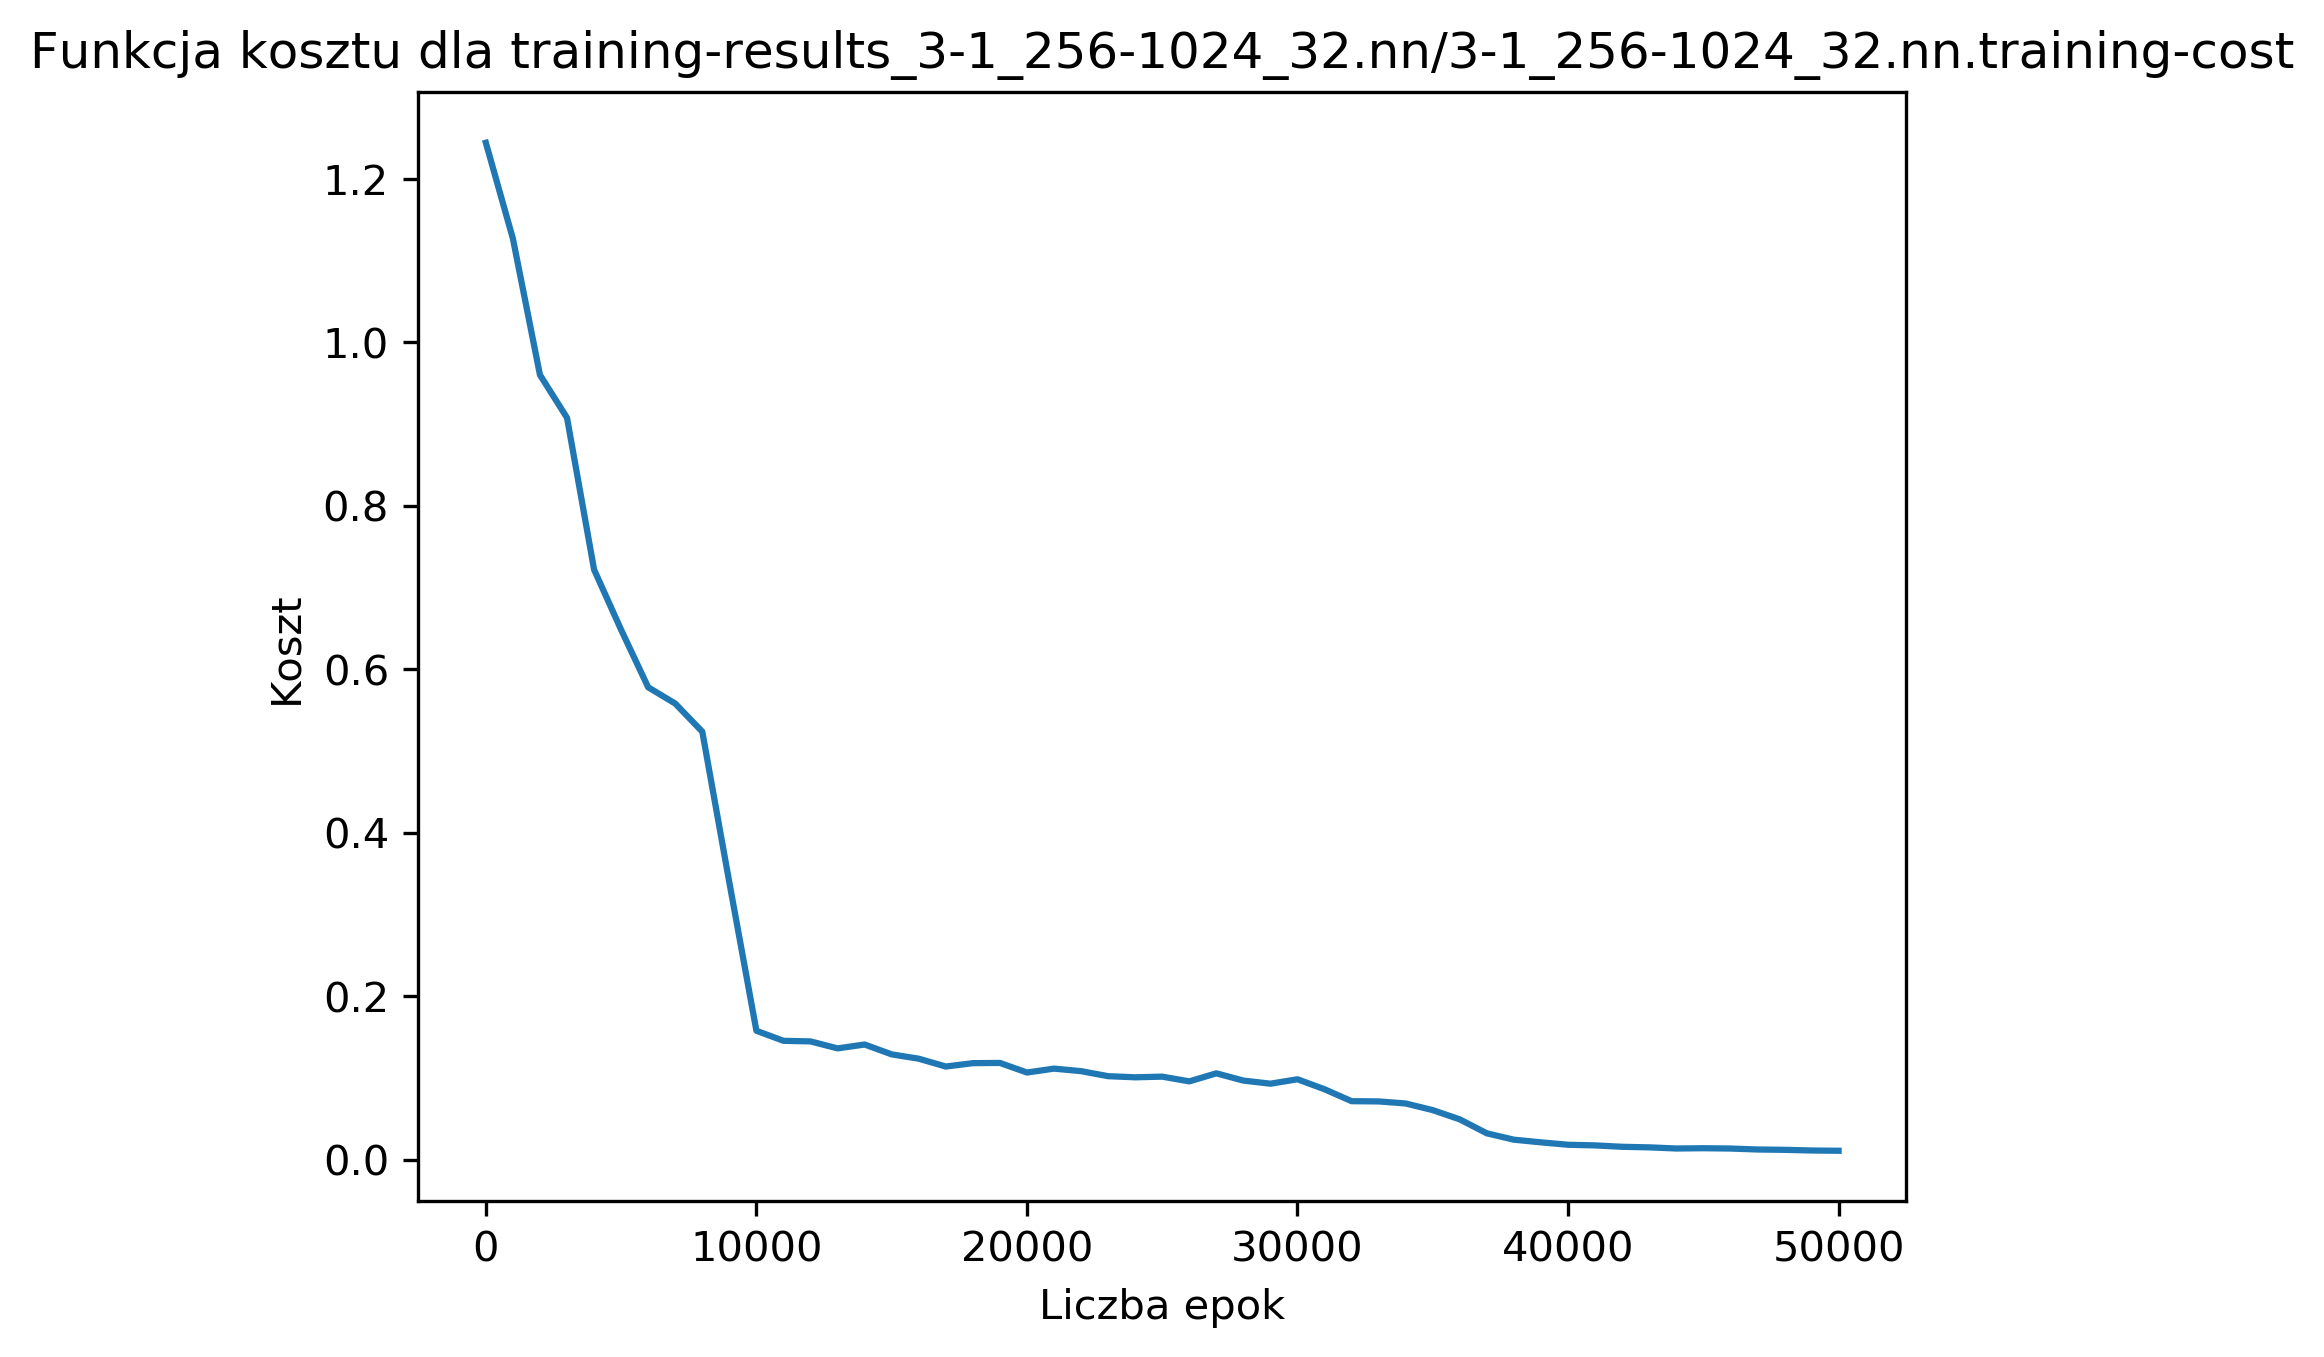
\includegraphics[width=120mm]{wykresy/3-1_256-1024_32_nn_training-cost.png}
            \end{figure}
            \begin{figure}[!htbp]
                \centering
                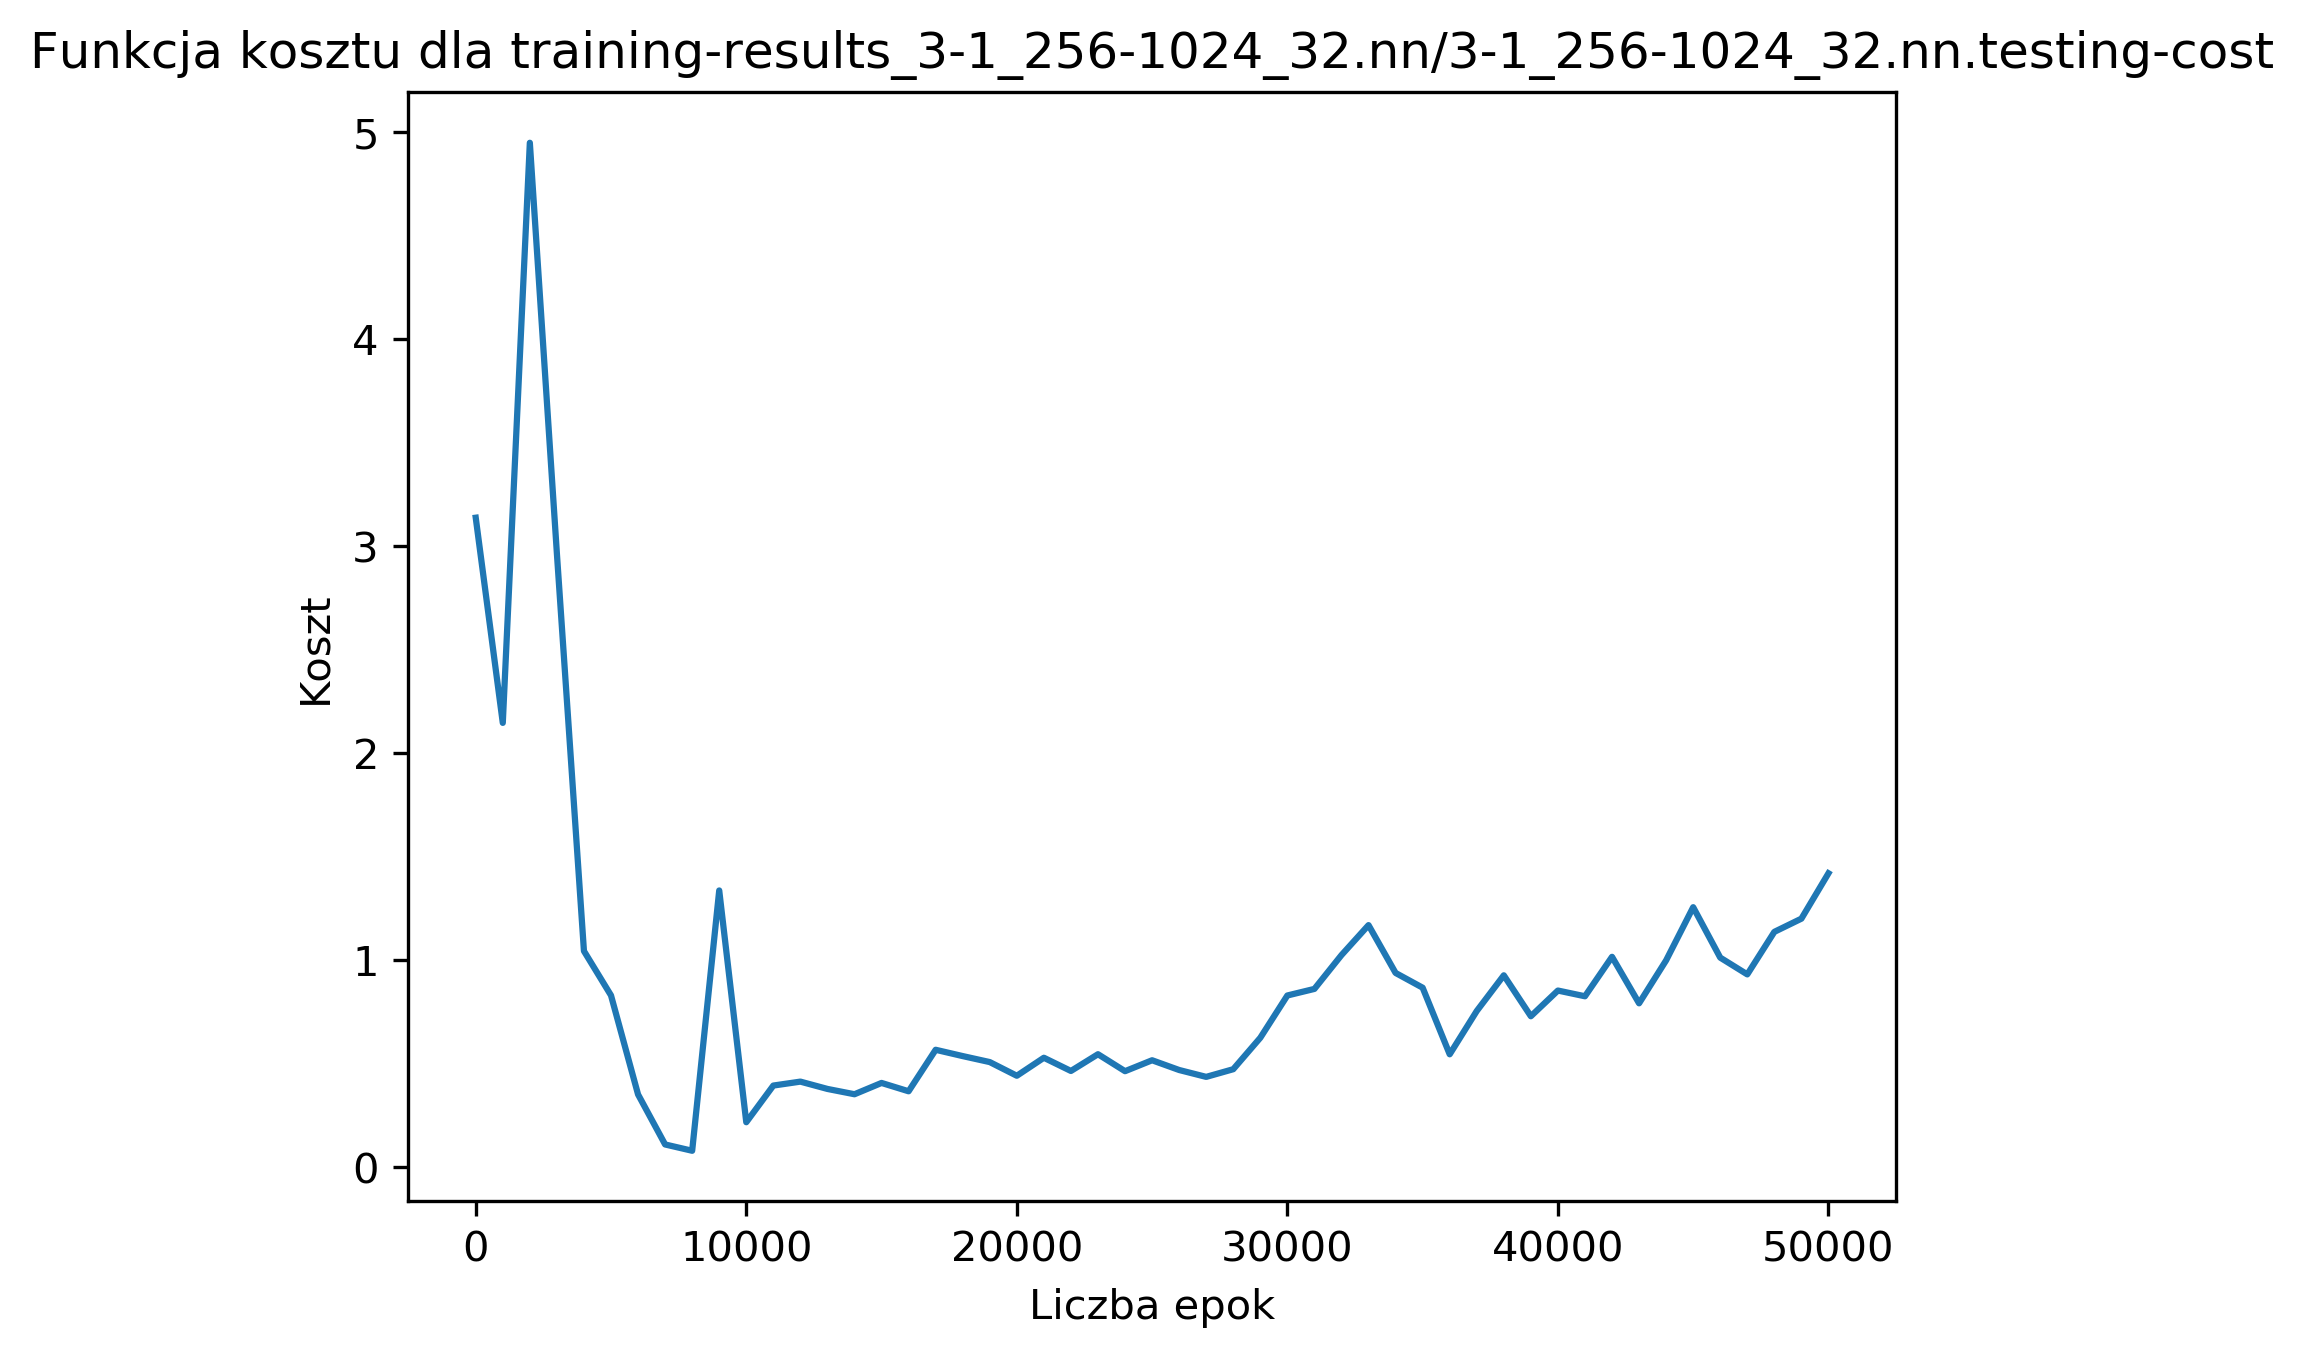
\includegraphics[width=120mm]{wykresy/3-1_256-1024_32_nn_testing-cost.png}
            \end{figure}
            \begin{figure}[!htbp]
                \centering
                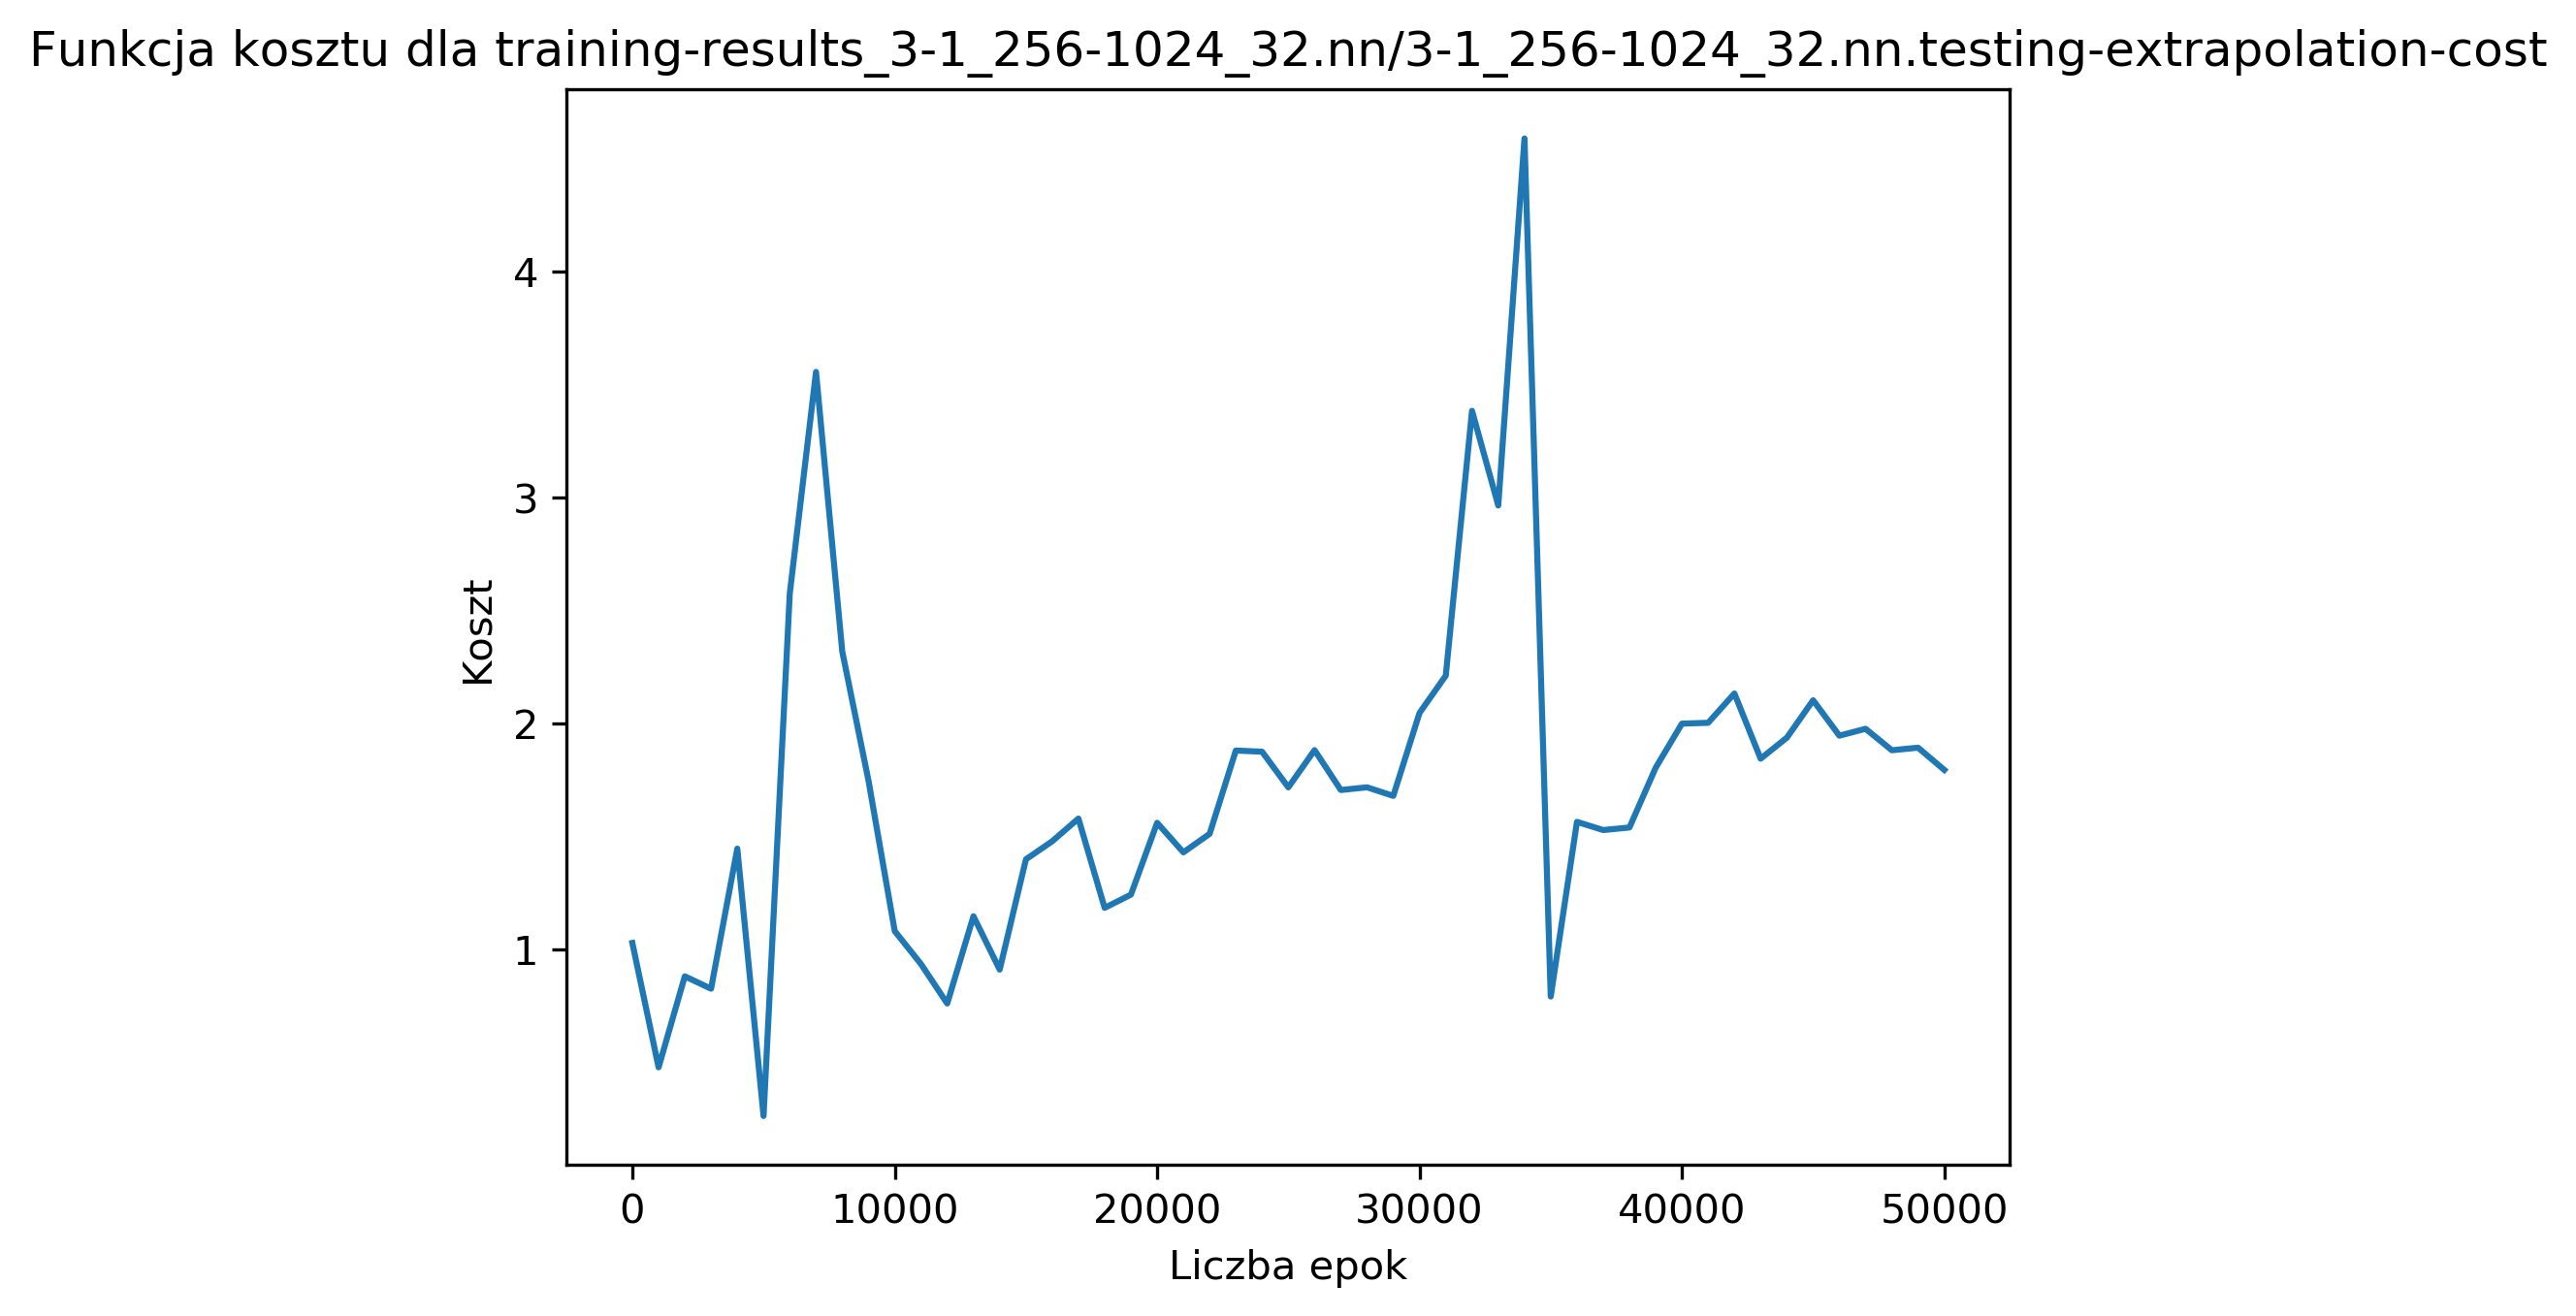
\includegraphics[width=140mm]{wykresy/3-1_256-1024_32_nn_testing-extrapolation-cost.png}
            \end{figure}
            \FloatBarrier
        %---------------------------------------------------%
            \begin{figure}[!htbp]
                \centering
                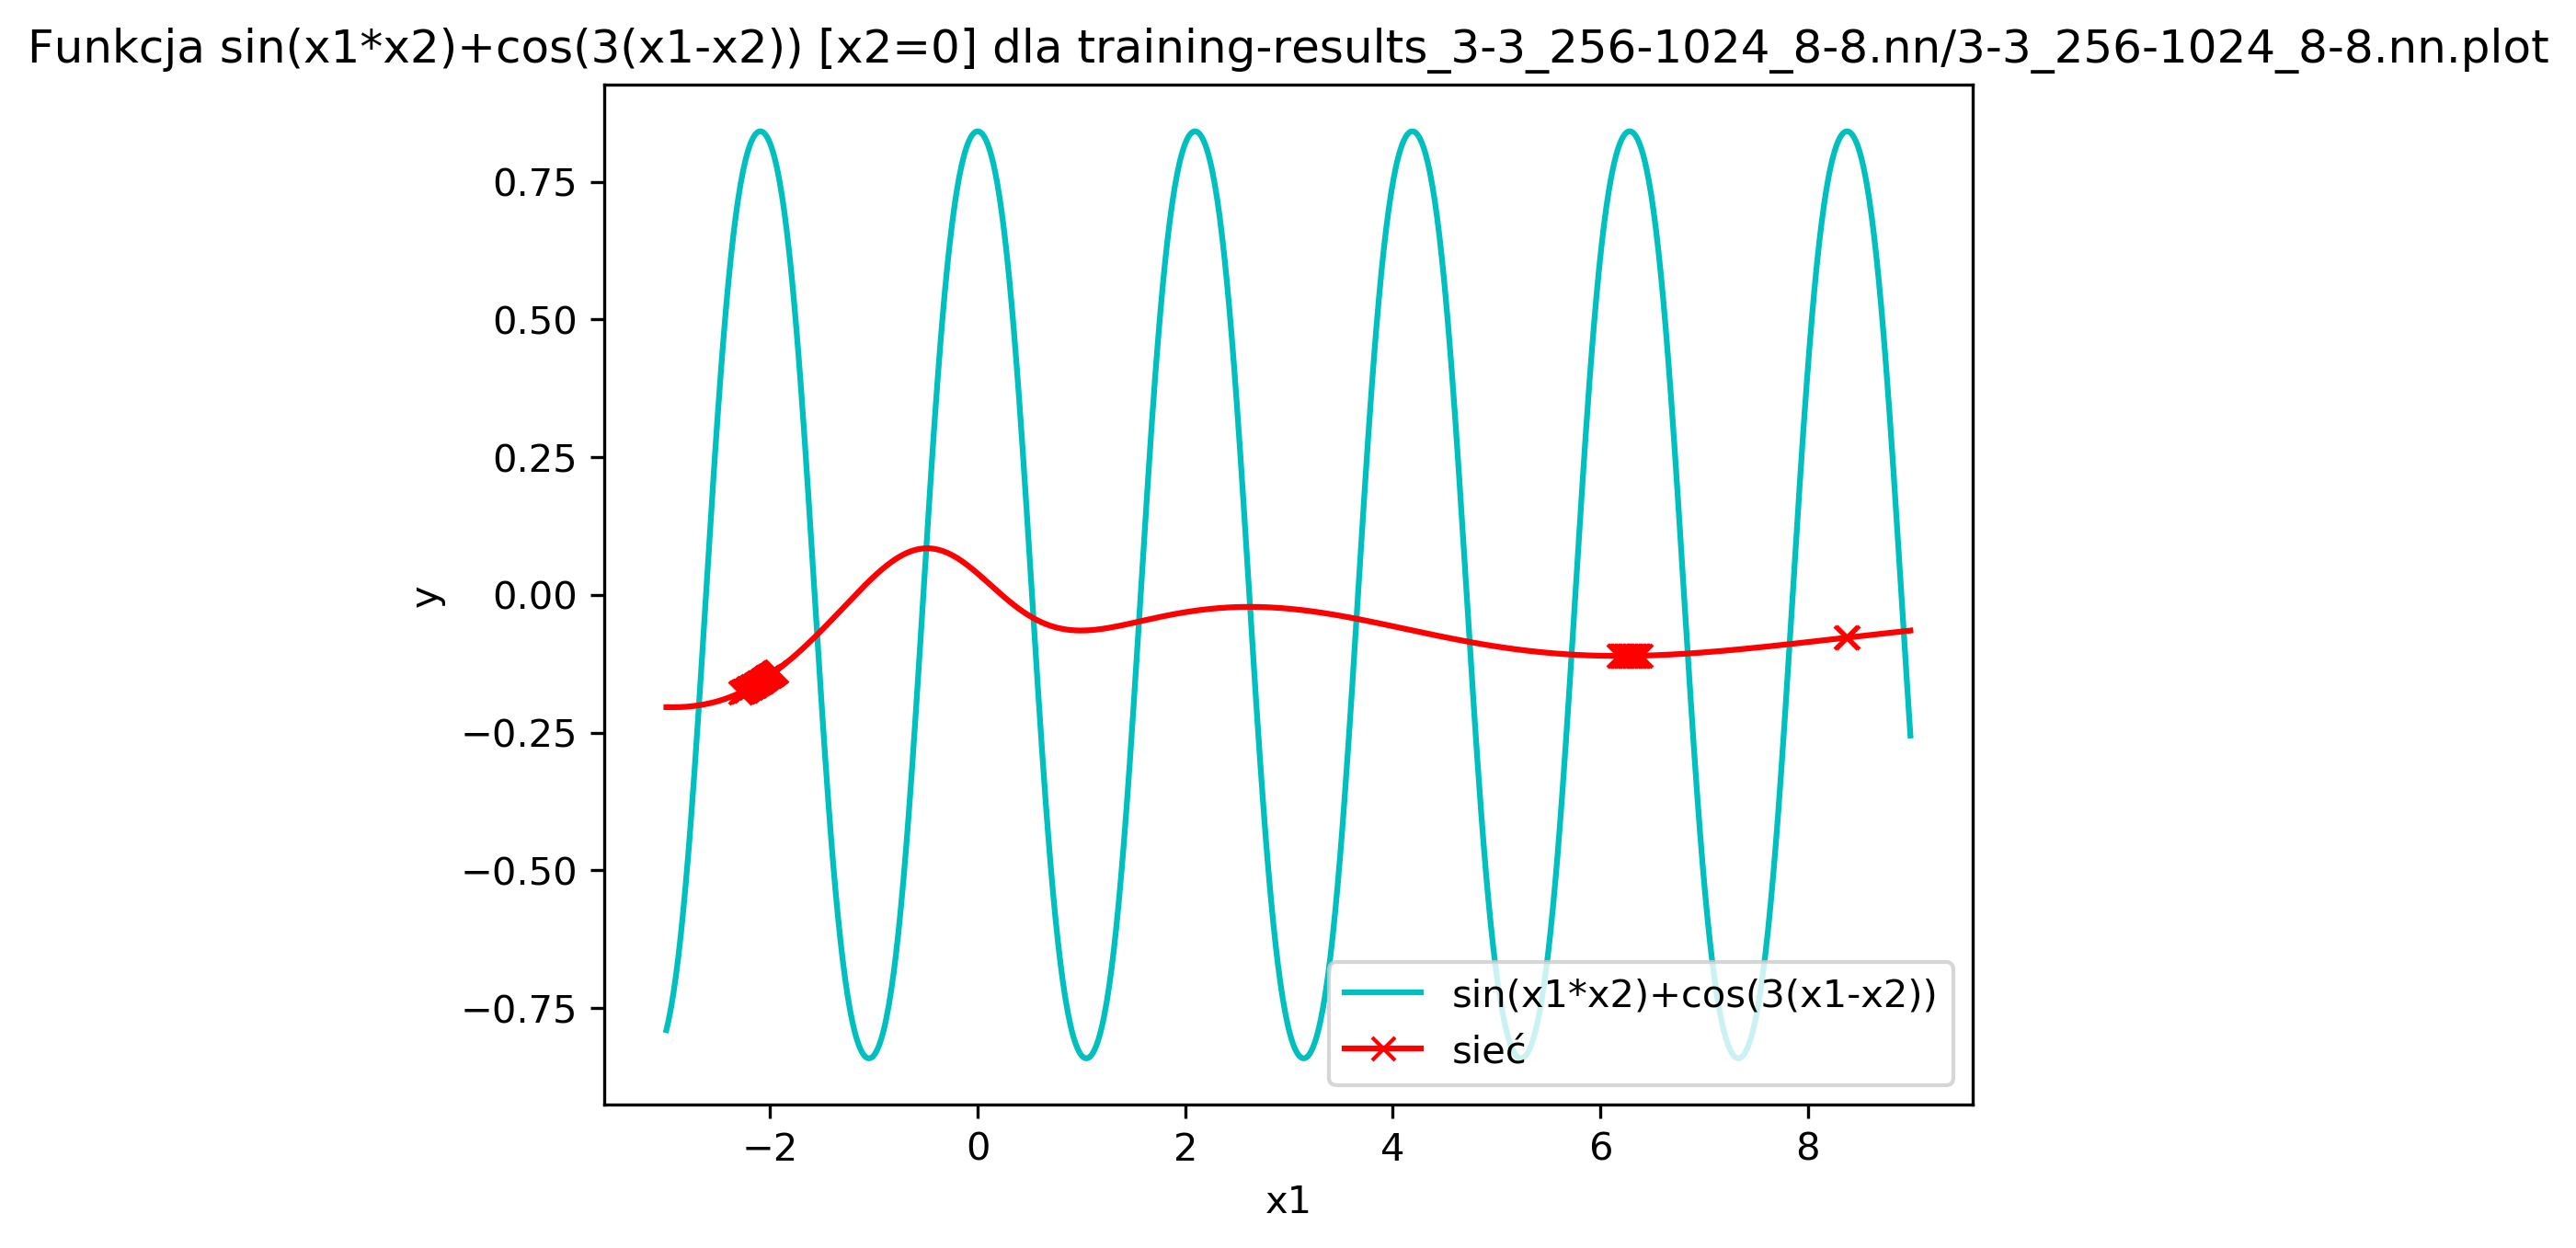
\includegraphics[width=135mm]{wykresy/3-3_256-1024_8-8_nn_plot1.png}
            \end{figure}
            \begin{figure}[!htbp]
                \centering
                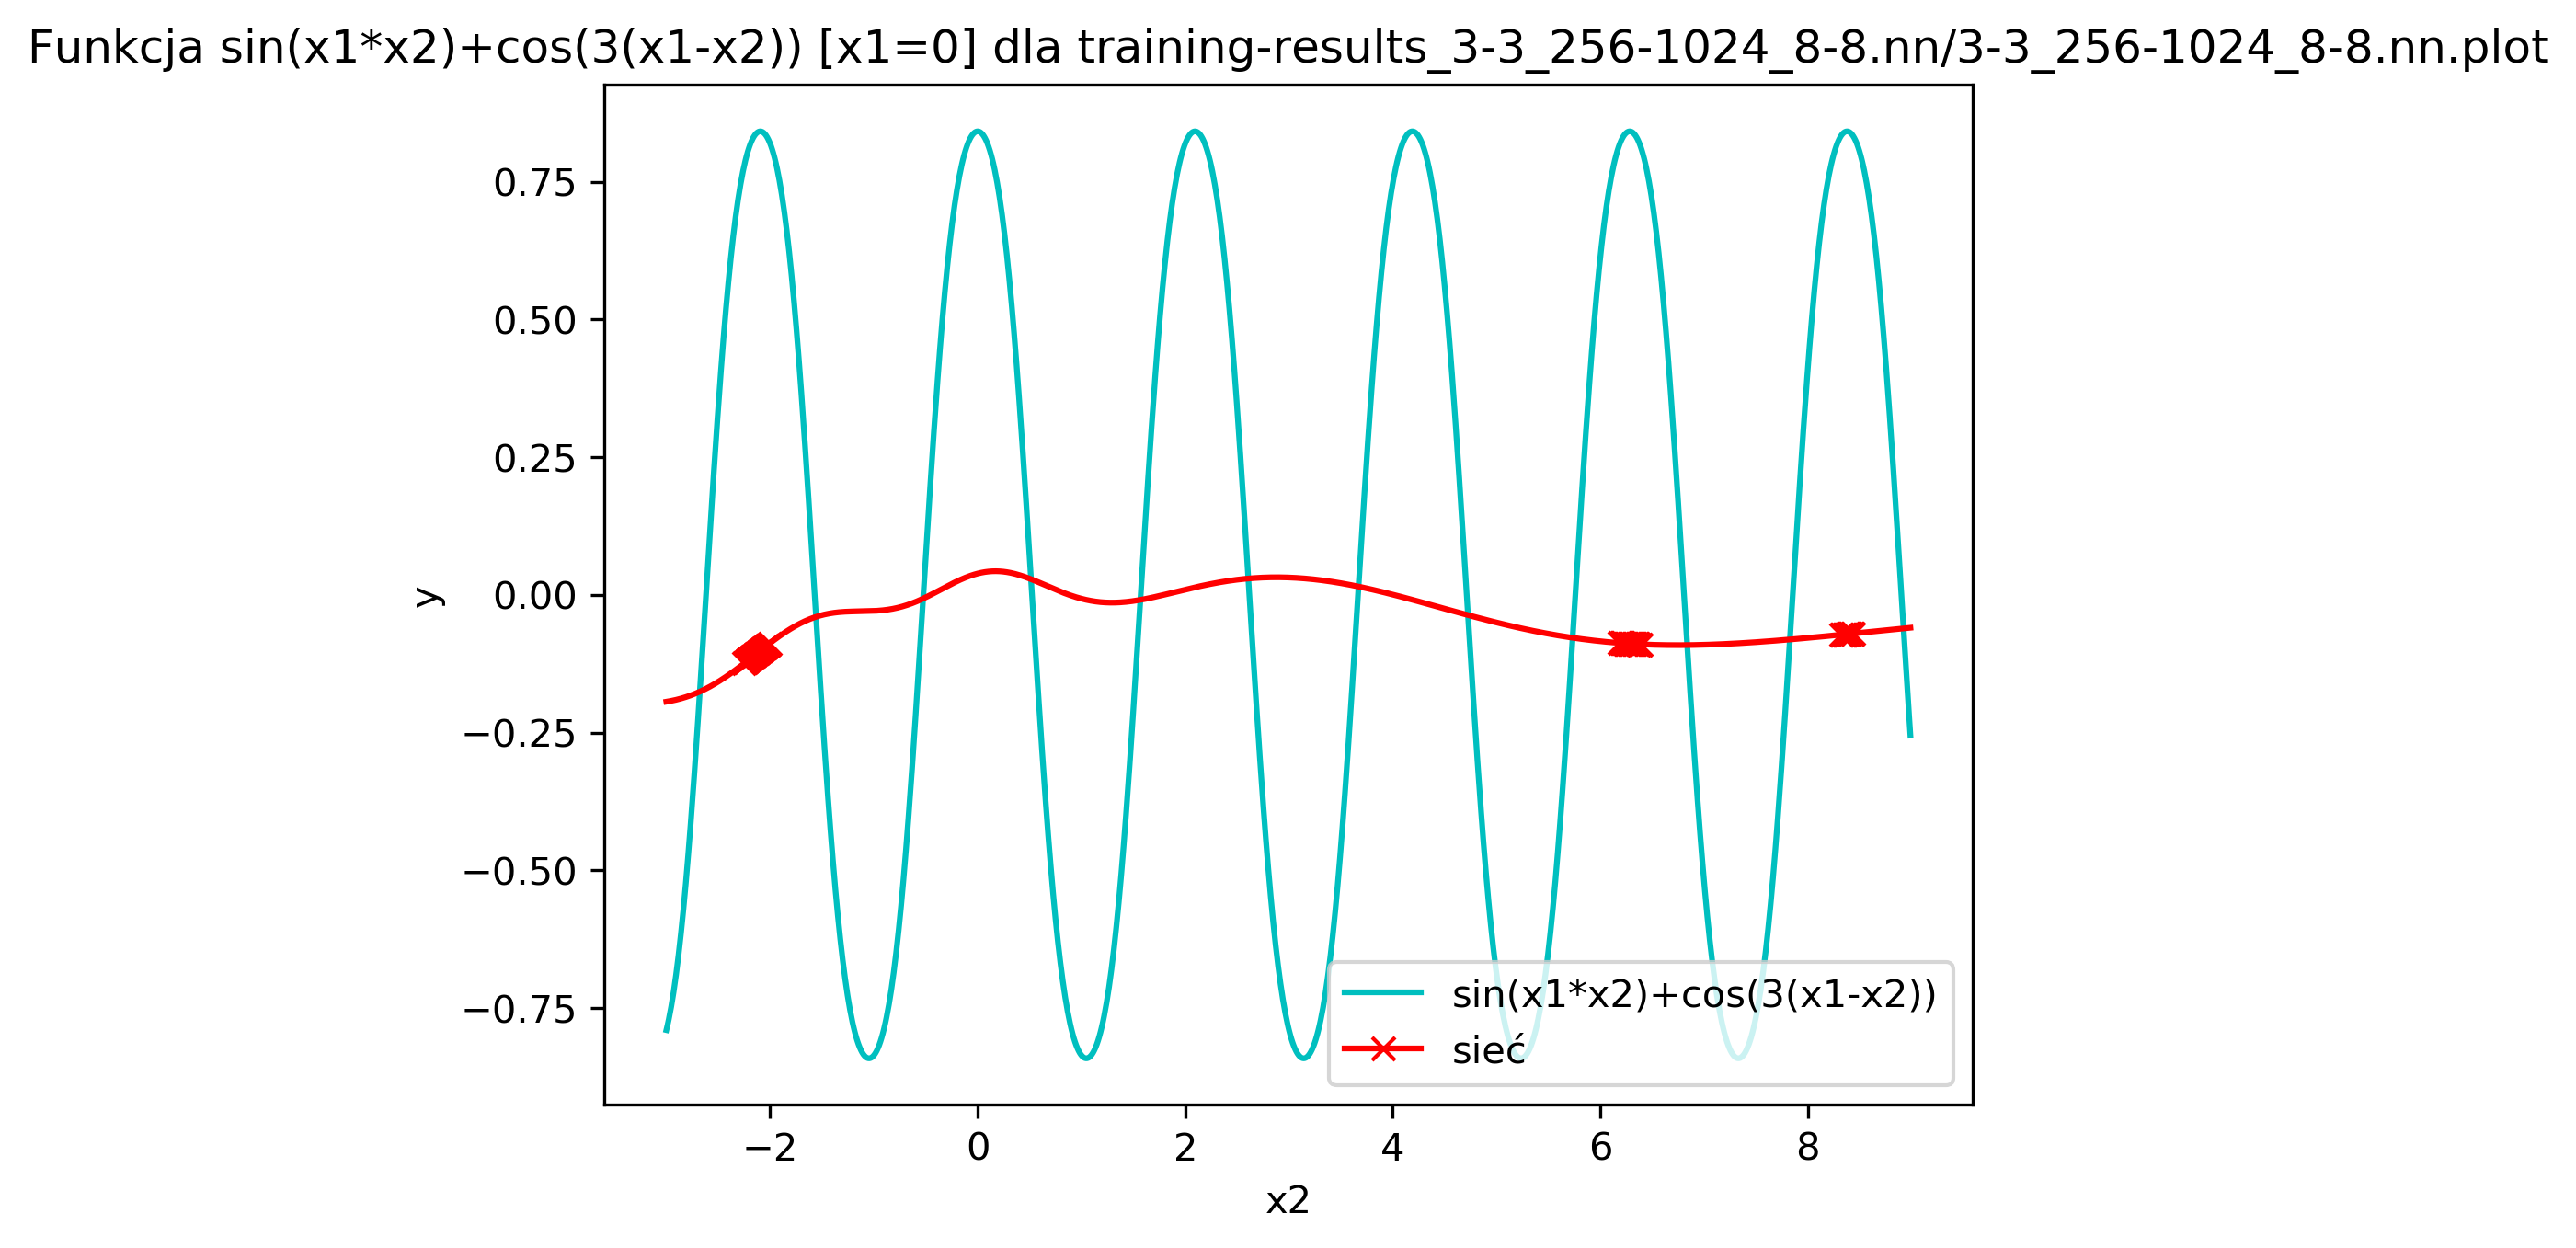
\includegraphics[width=135mm]{wykresy/3-3_256-1024_8-8_nn_plot2.png}
            \end{figure}
            \begin{figure}[!htbp]
                \centering
                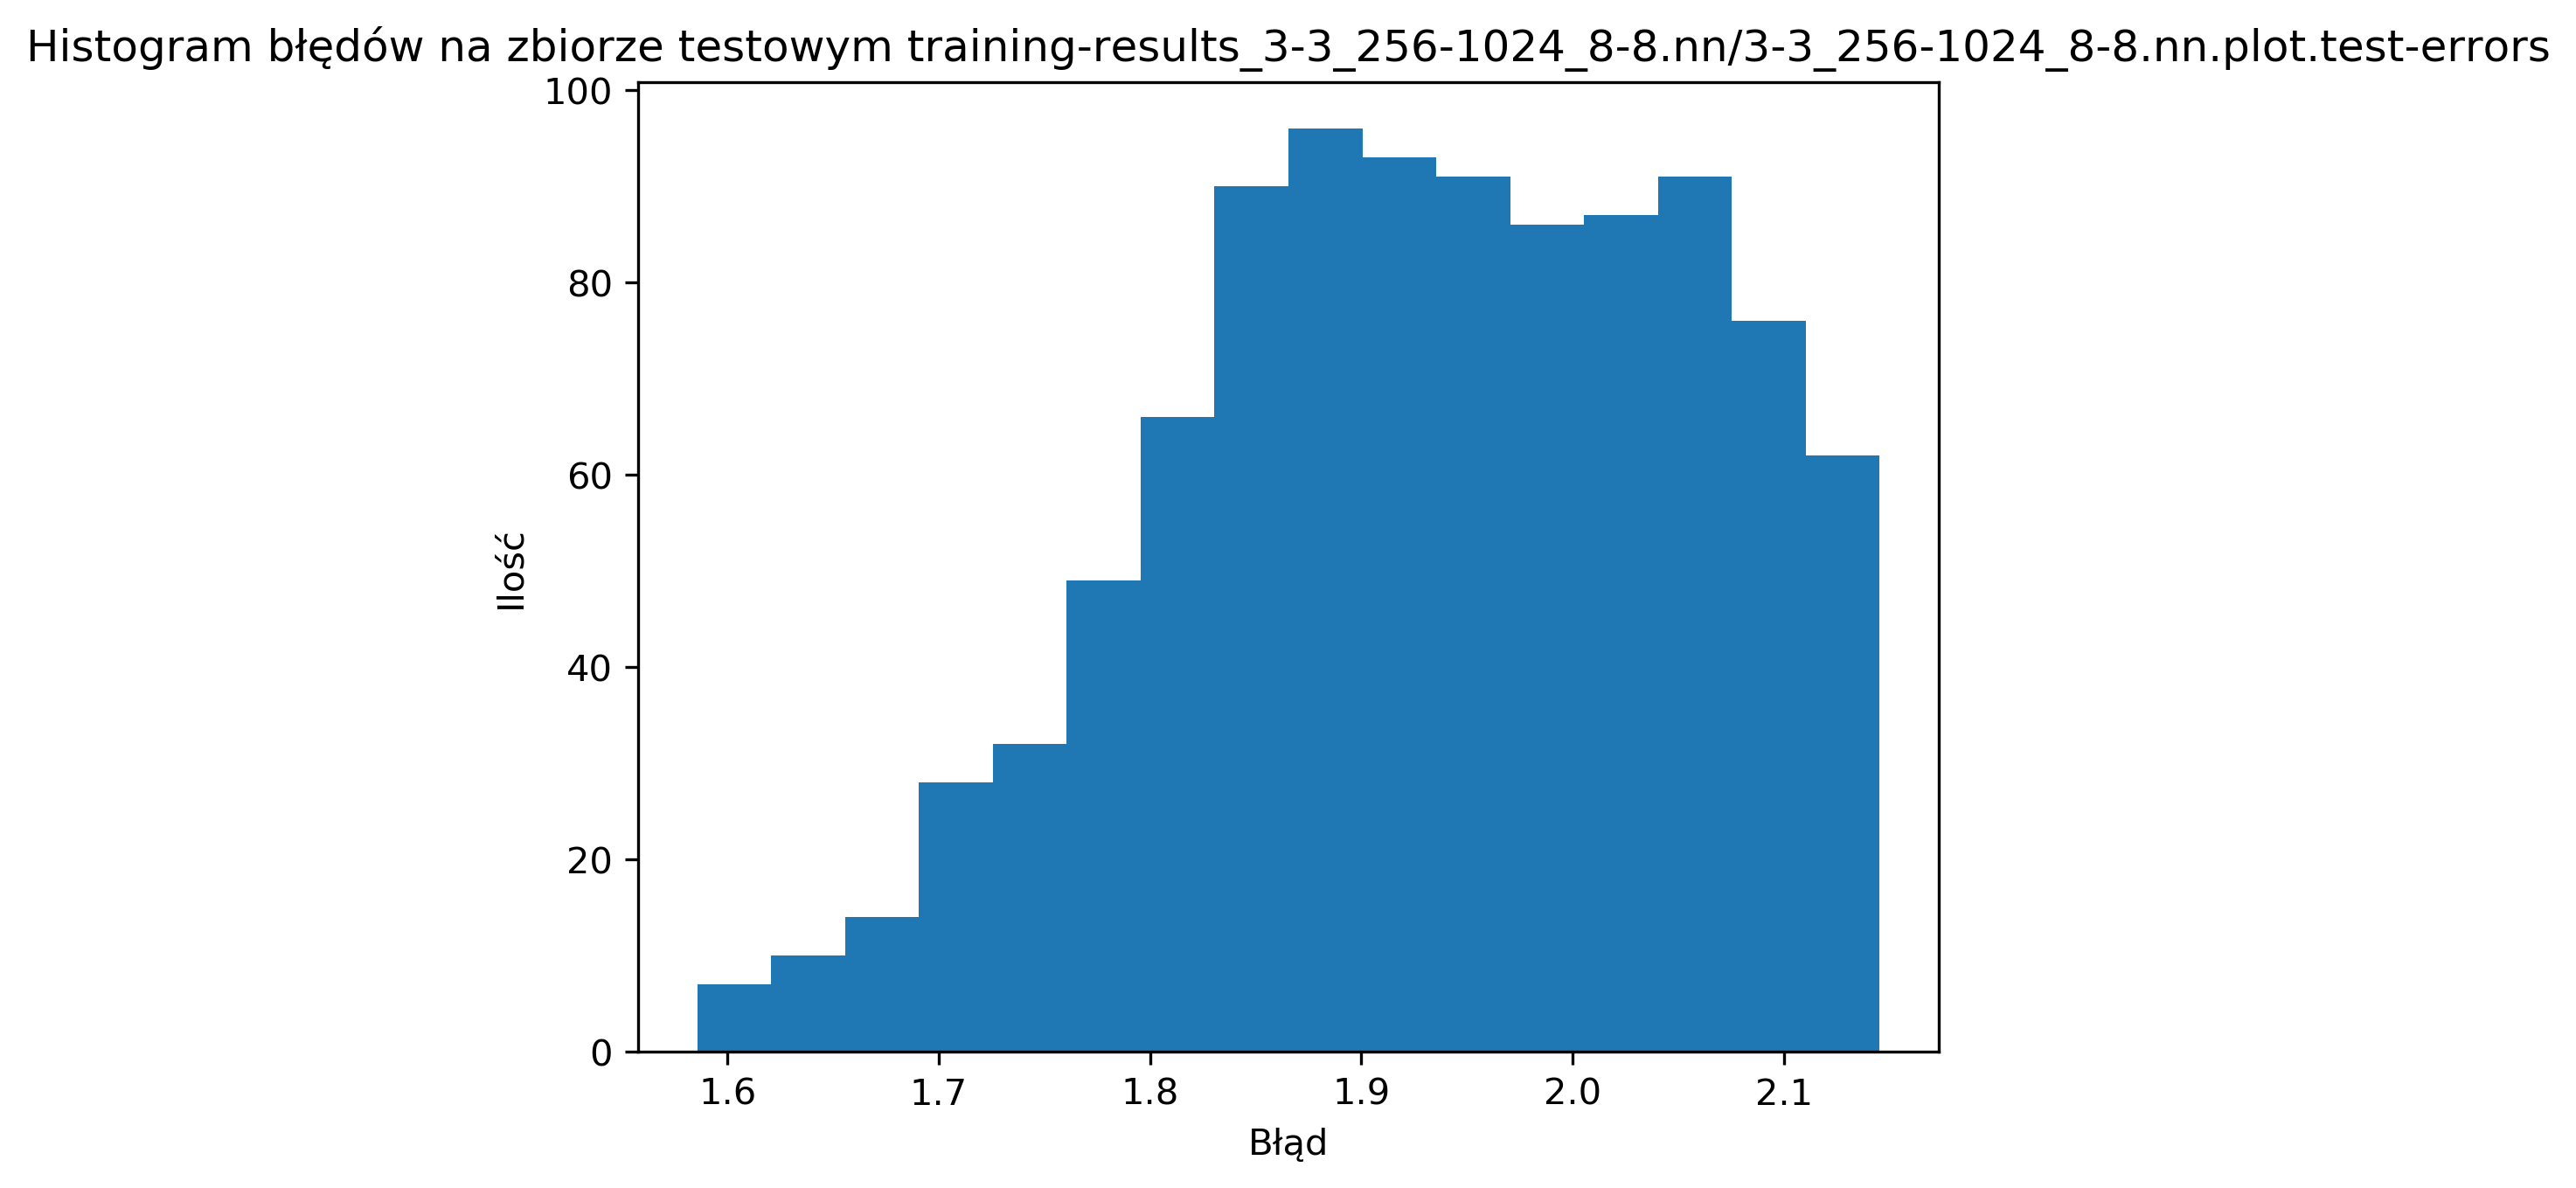
\includegraphics[width=145mm]{wykresy/3-3_256-1024_8-8_nn_plot_test-errors.png}
            \end{figure}
            \begin{figure}[!htbp]
                \centering
                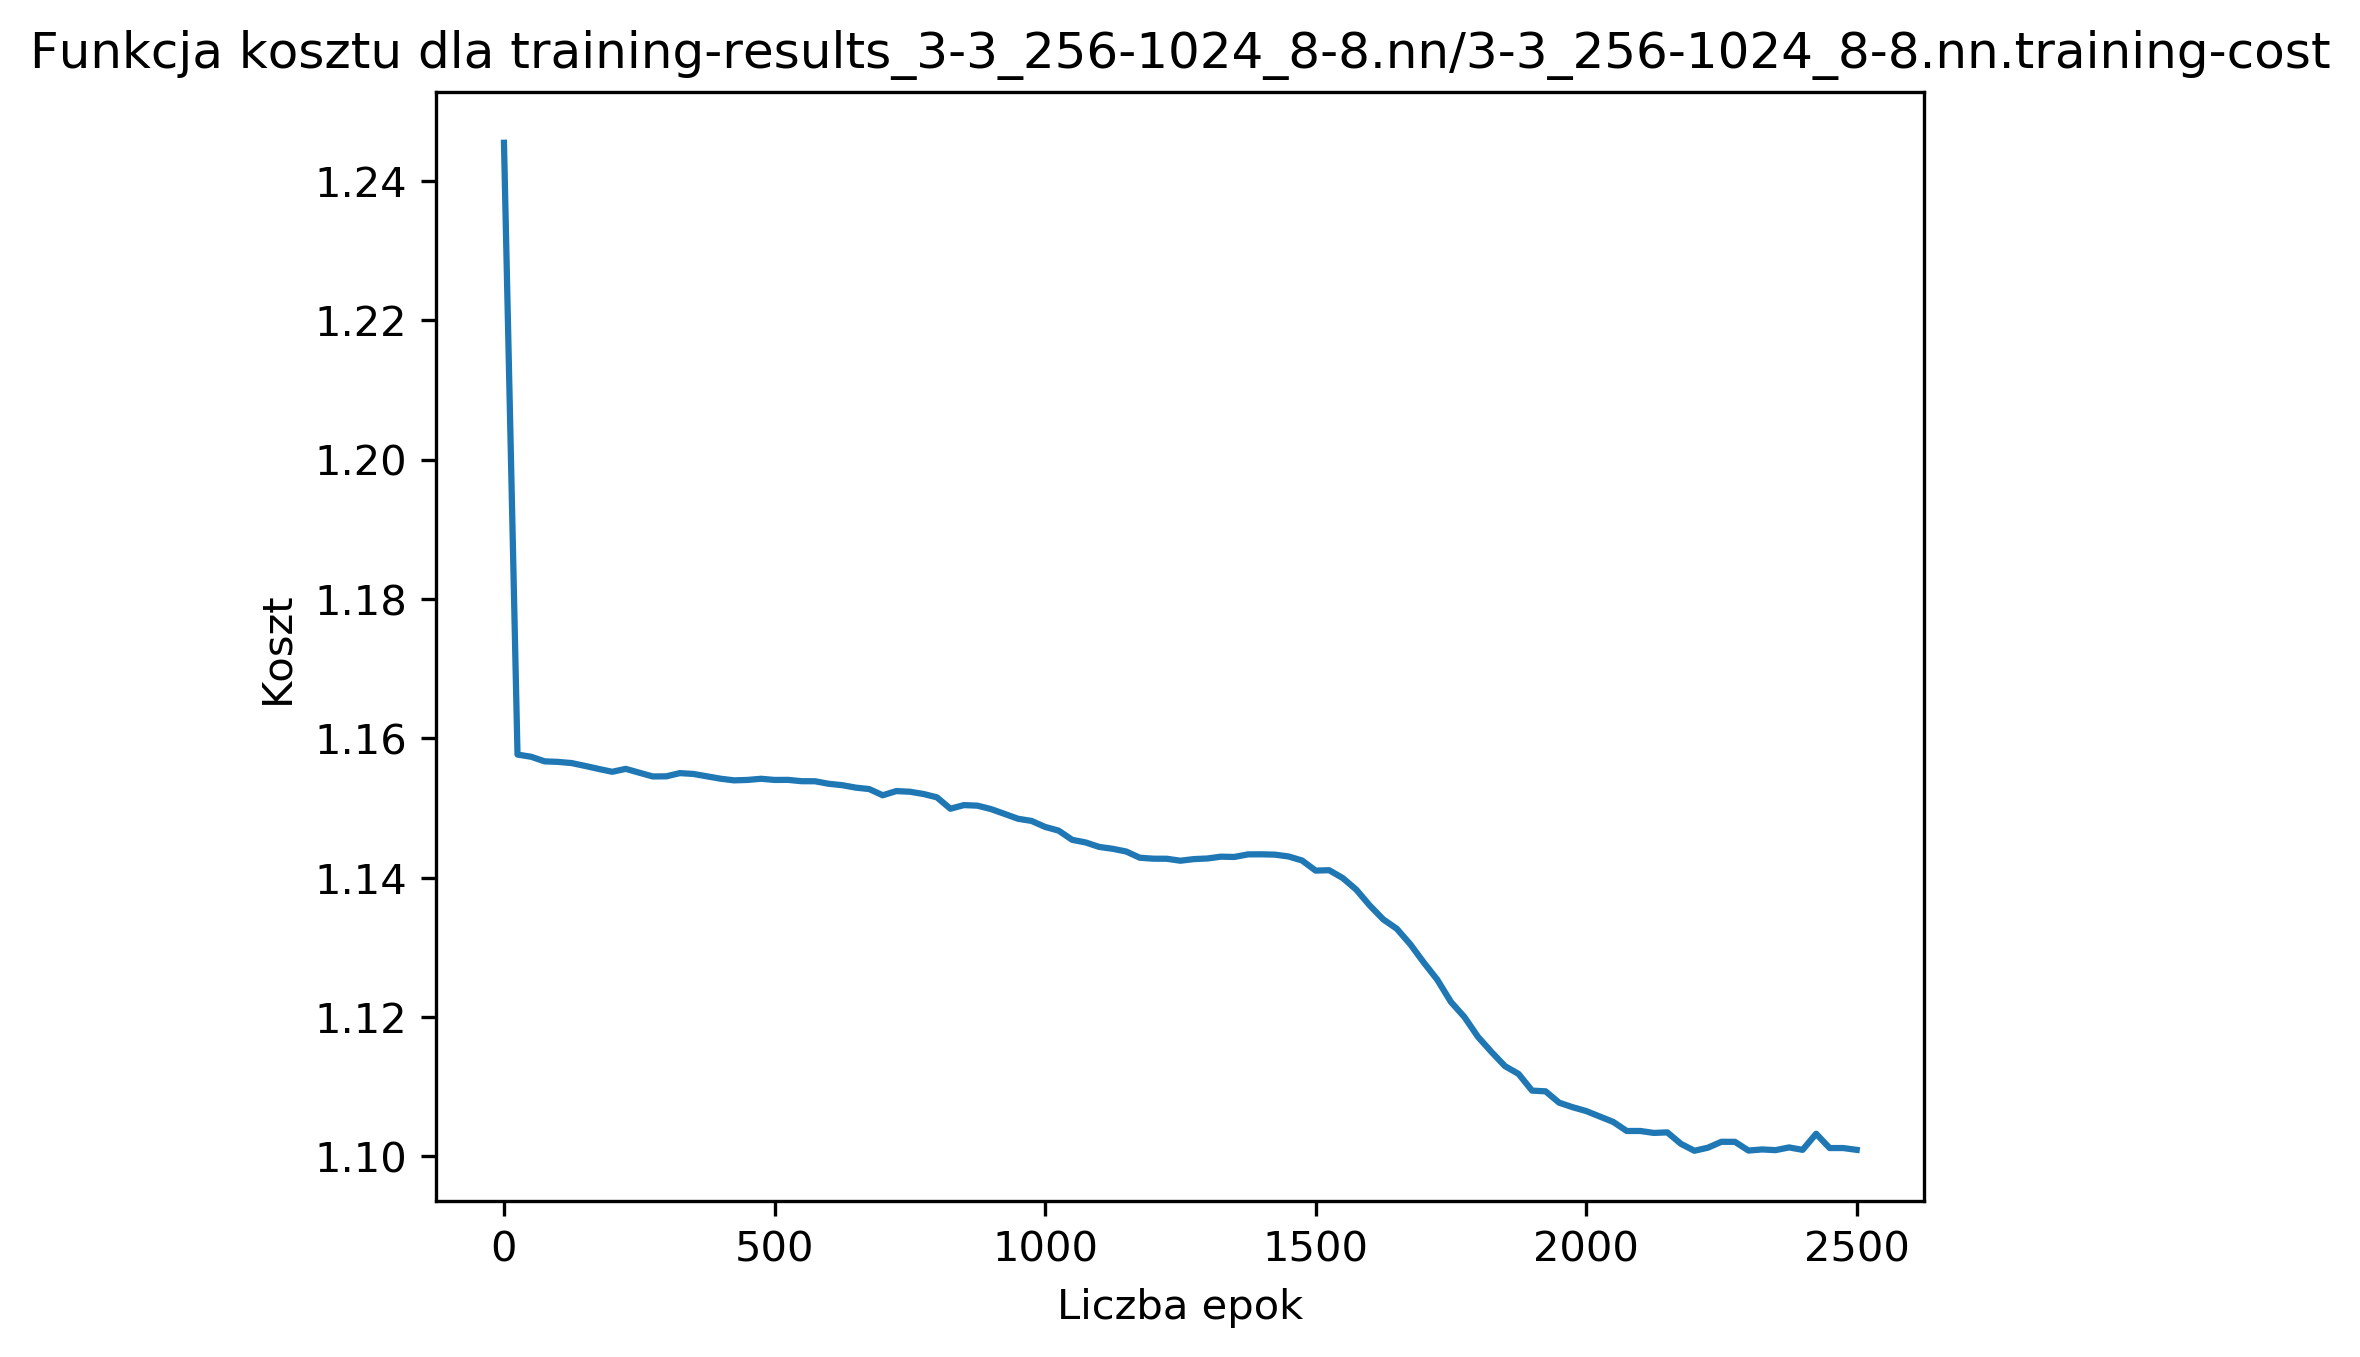
\includegraphics[width=120mm]{wykresy/3-3_256-1024_8-8_nn_training-cost.png}
            \end{figure}
            \begin{figure}[!htbp]
                \centering
                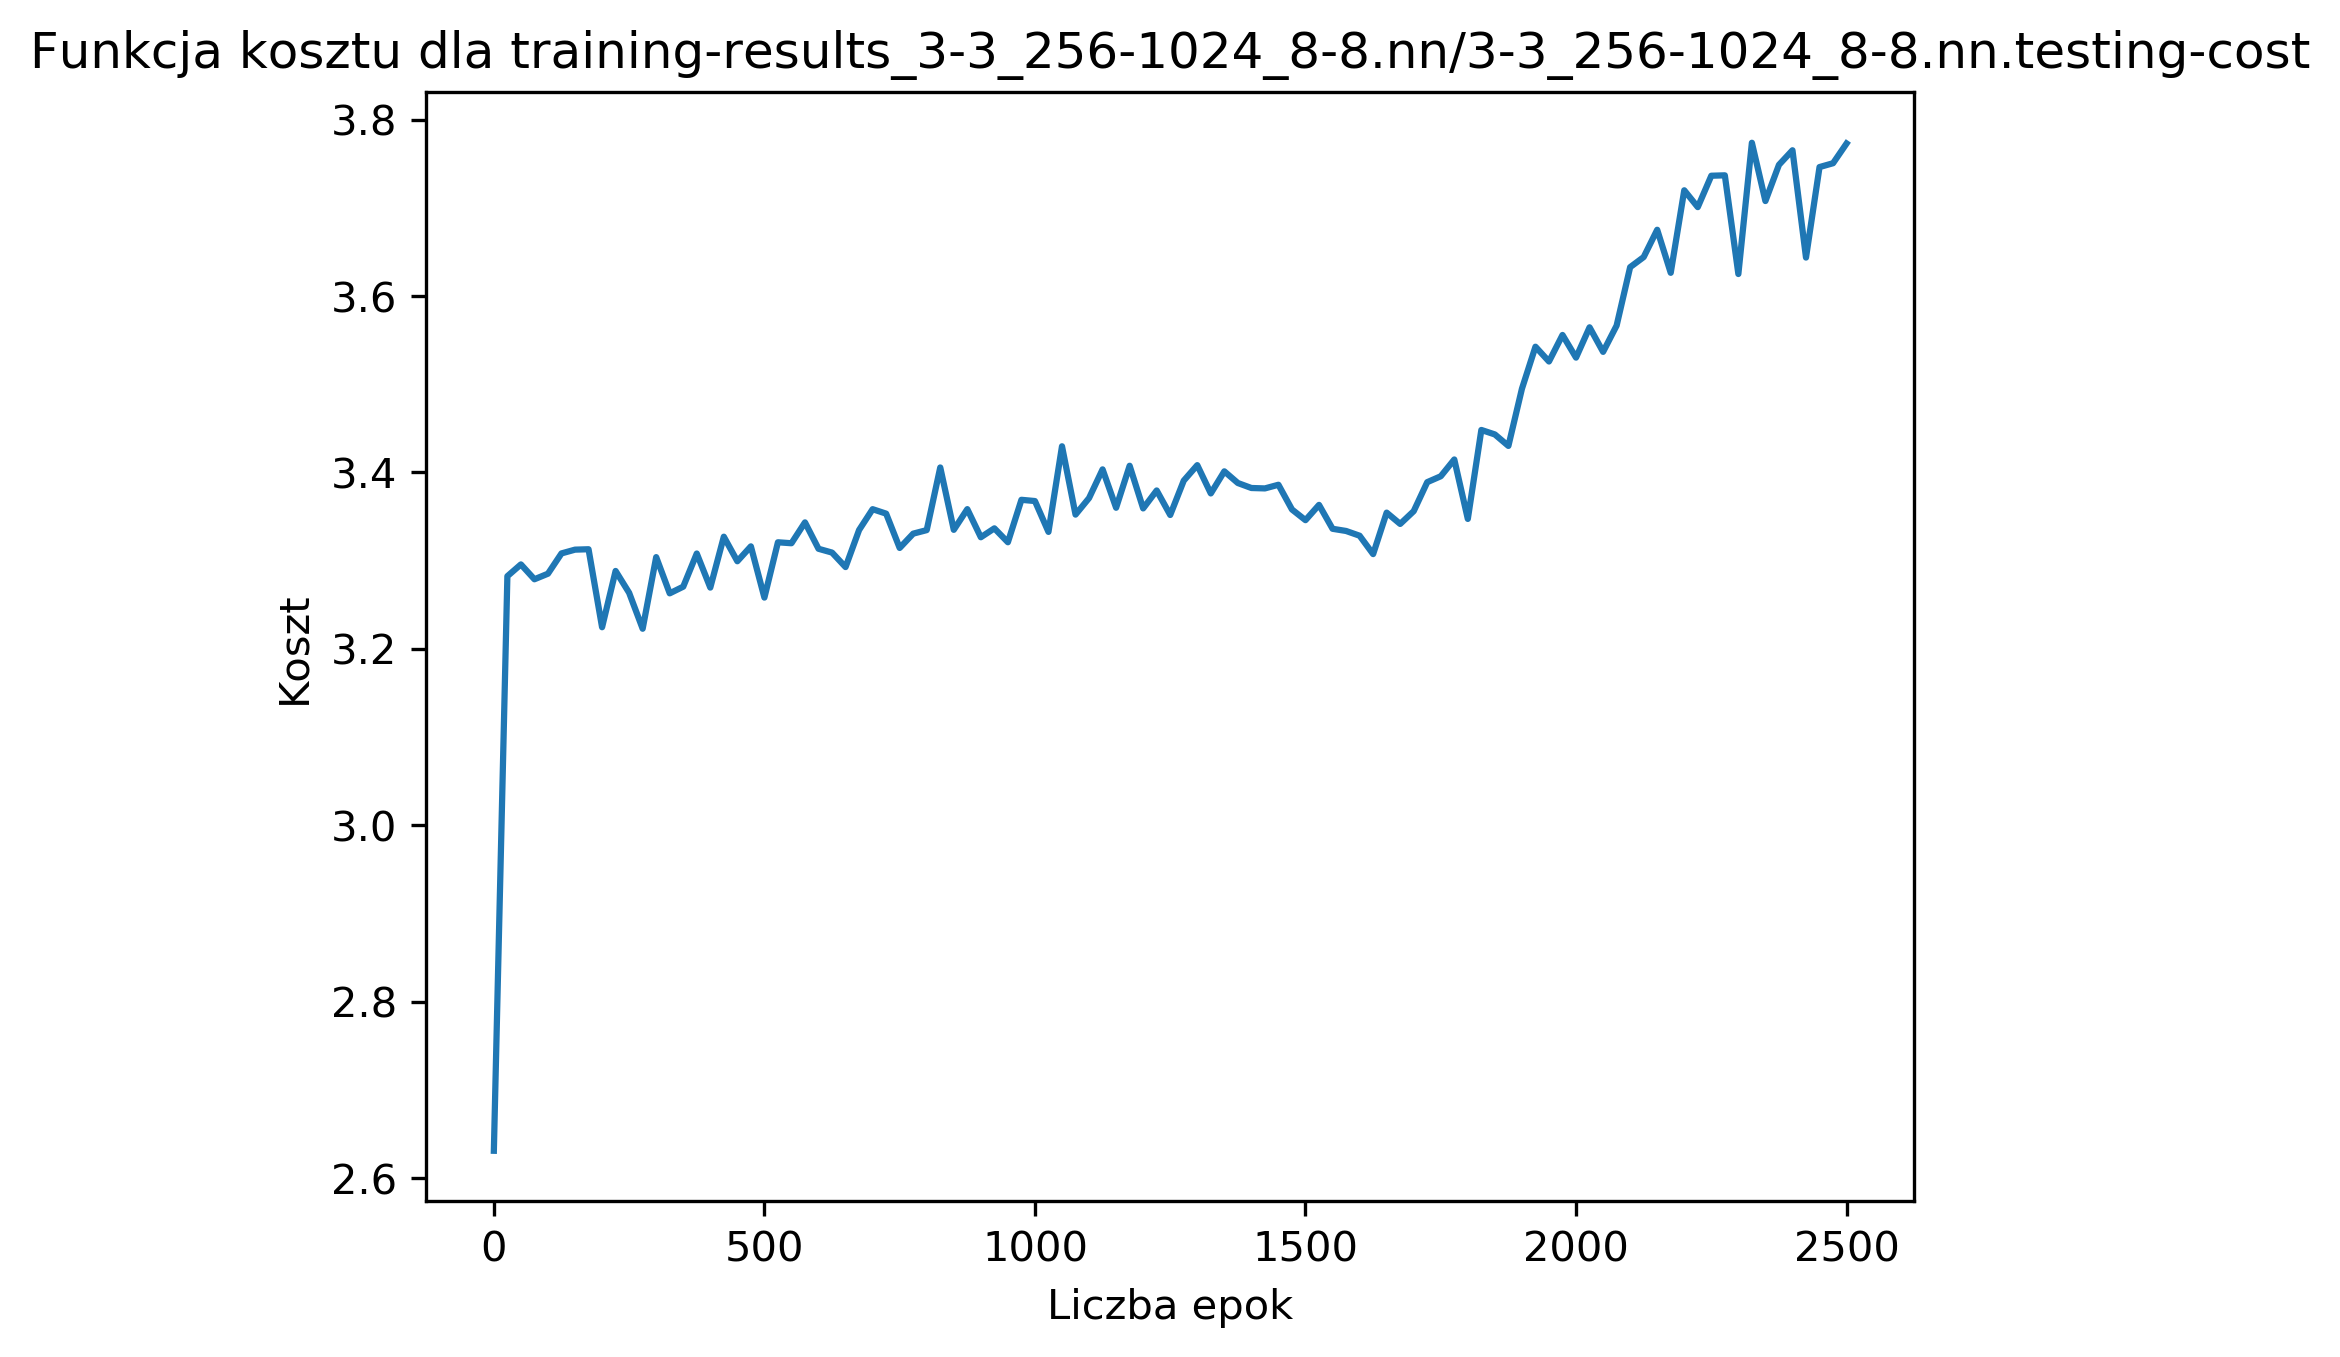
\includegraphics[width=120mm]{wykresy/3-3_256-1024_8-8_nn_testing-cost.png}
            \end{figure}
            \begin{figure}[!htbp]
                \centering
                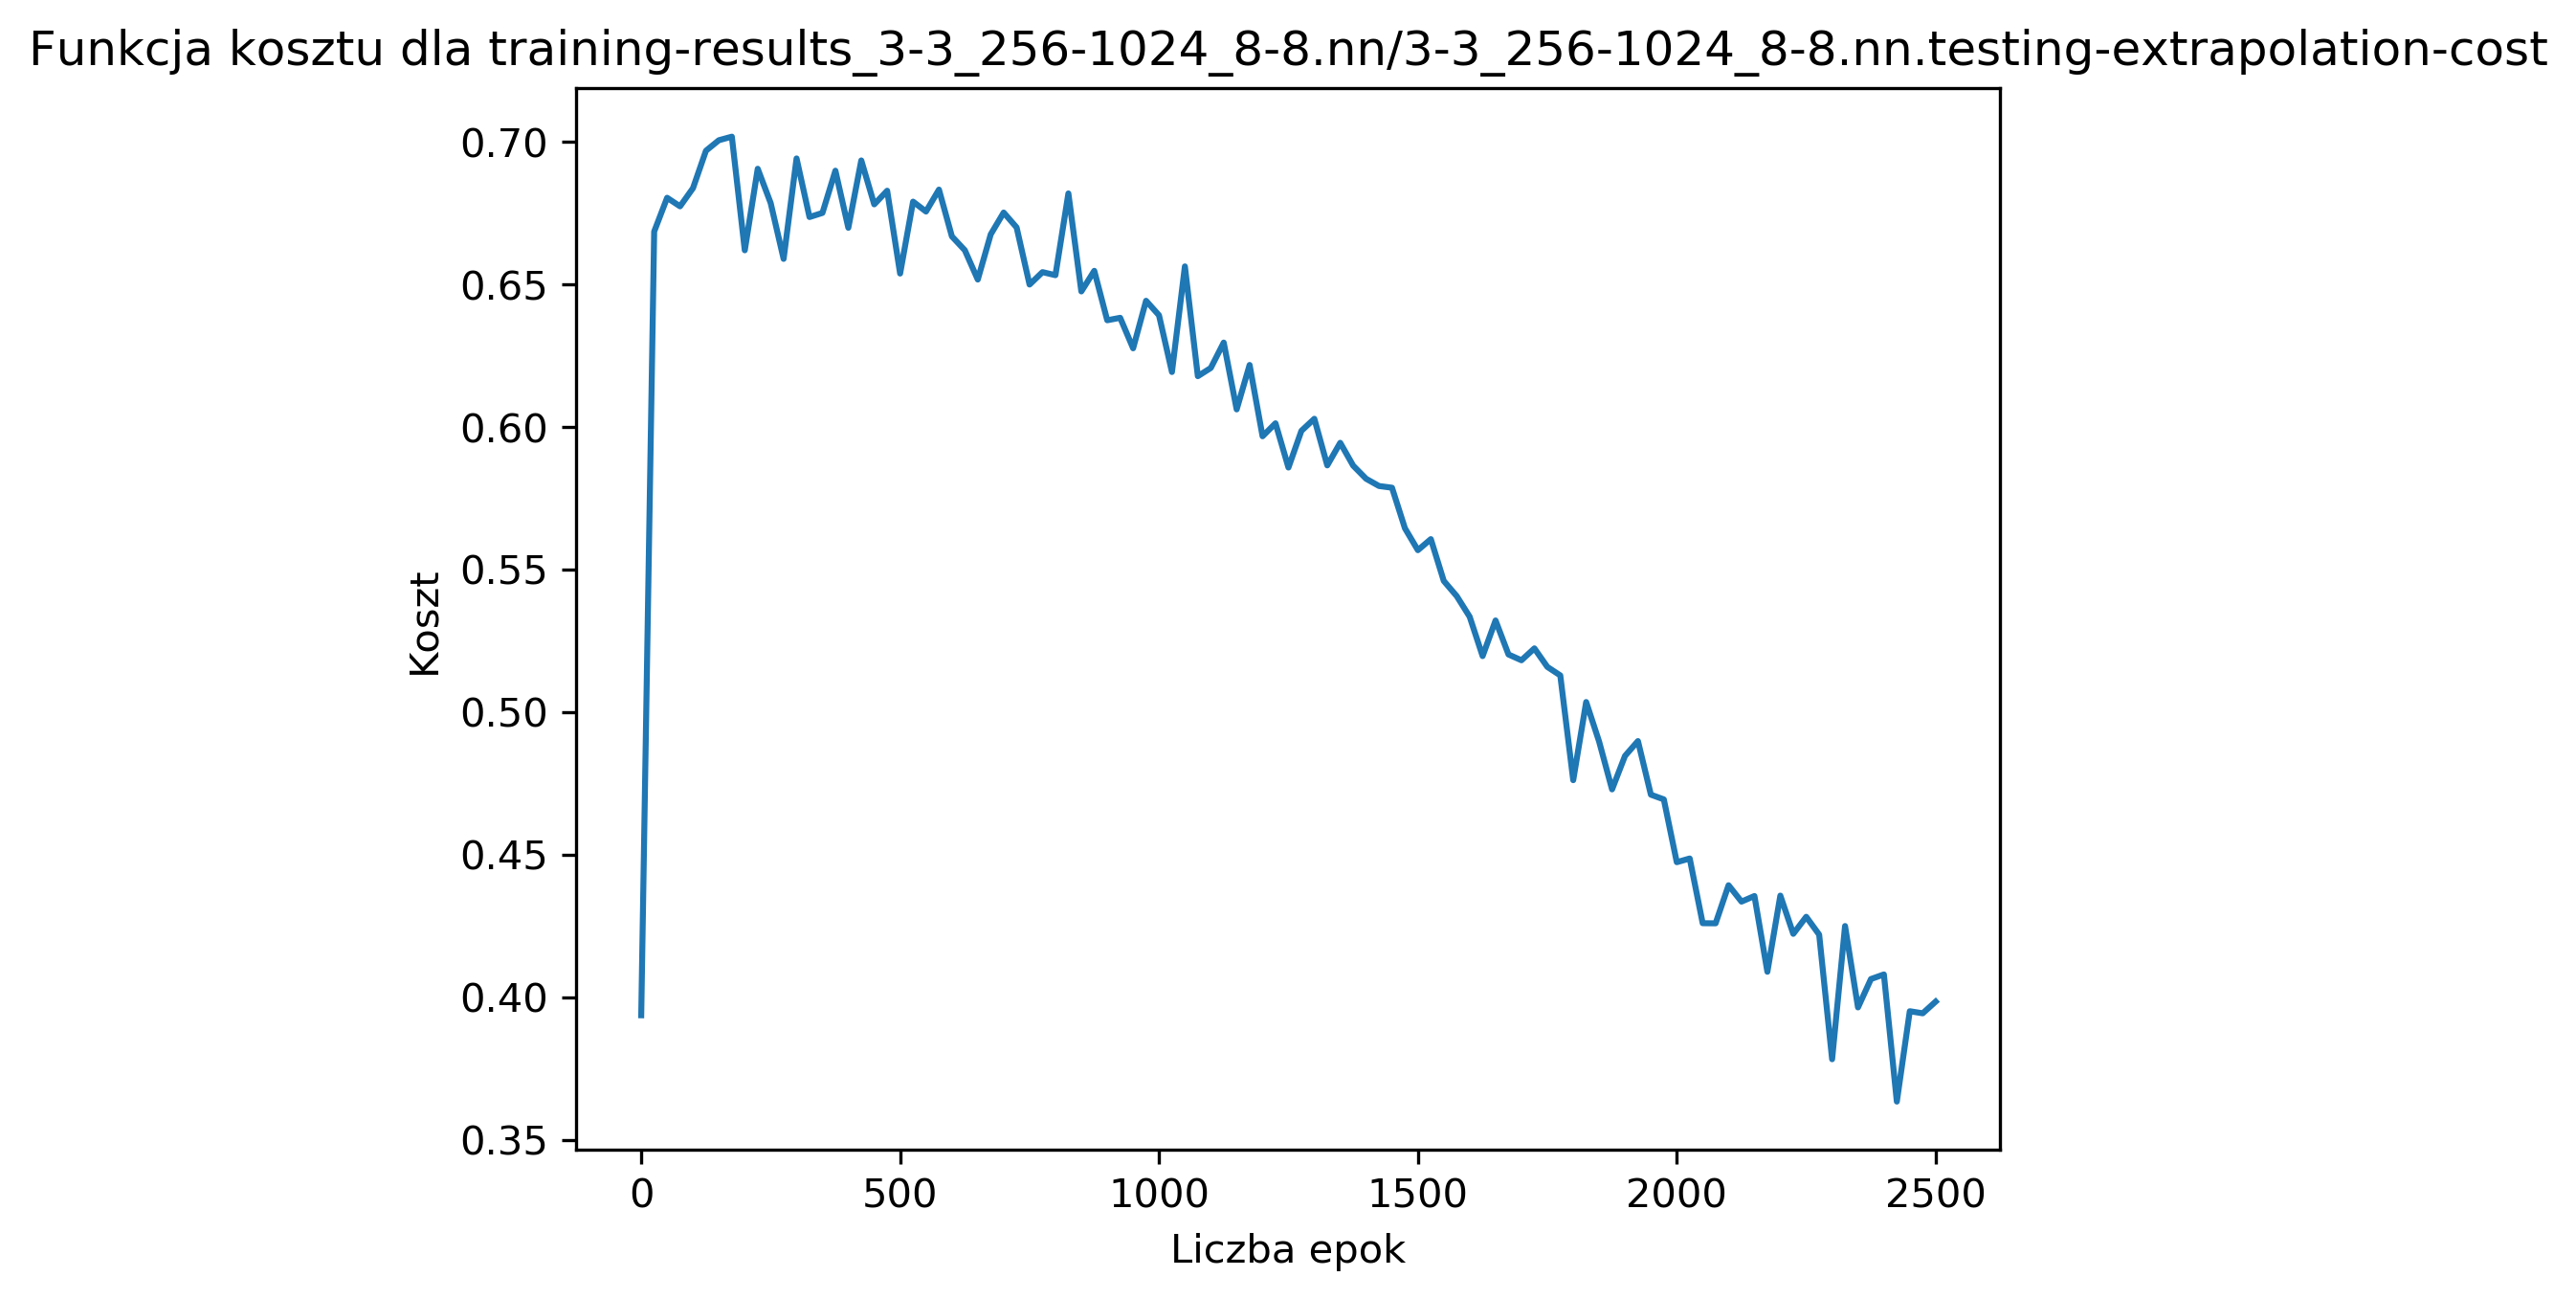
\includegraphics[width=140mm]{wykresy/3-3_256-1024_8-8_nn_testing-extrapolation-cost.png}
            \end{figure}
            \FloatBarrier
        %---------------------------------------------------%
        }
    %---------------------------------------------------%

    }
%--------------------------------------------------------------------------------------%
    \section{Dyskusja}
    {
        Przedstawione funkcje na wykresach maja pierwsza połowe argumentów przeznaczonych do procesu nauki natomiast druga cześć
        podlega testowaniu ekstrapolacji.\\

        Na bazie aproksymacji funkcji pierwiastkowej po zbadaniu liczby punktów trenignowych 4,9,16,64 zauważyliśmy ze juz przy
        liczbe 9 punktów wynik działania programu jest satysfakcjonujacy i przybliżenie funkcji jest naszym zdaniem wystraczajaco dobre i nie ma
        potrzeby aby powtarzac obliczenia z większa liczba punktów. \\

        Zauważmy że nie udało się nam otrzymać satysfakcjonujacej extrapolacji funkcji pierwsiatkowej w przypadku warstw RBF.
        W czasie nauki udało nam sie osiagnać ze funkcja kosztu od numeru iteracji cały czas malała jednak wynik tej ekstrapolacji nas nie
        satysfakcjonuje.\\

        Warto zwrócic uwage na sposob działania warstwy RBF ponieważ jej wagi sa interpretowane jako neurony wzgledem których liczymy
        prawdopodobieństwa wejscia oraz zwrócicmy uwage na w miare roznomierny rozkład tych neruonów na wykresie pierwiastka co przekłada sie na zadawalajaco aproksymacje jednak z drugiej strony połozenie tych neuronow tylko w zakresie uczenia nie polepsza
        extrapolacji.\\

        W perzypdaku funkcji sinus warstwa afiniczna możemy zaobserwaować bardzo dobra aproksymacje na przedziale treningowym
        lecz nie koniecznie dobra eksrapolacje. Patrzac na wykres zmian funkcji kosztu w zakresie uczenia możemy zauwazyc "schodki".
        Zauwazylismy ze przy użytych parametrach nauki funkcje trygonometryczne sin oraz cos sa podatne na wpadanie w minima lokalne.
        Obserwujac koszt dla ekstrapolacji widzimy zjawisko over-fittingu tzn ze sieć mimo ciagłem minimalizjacji kosztu treningowego w
        pewnym momencie zaczyna zwiekszac koszt esktrapolacji.\\

        Dla funkcji sinus ale mieszanej architektury sieci rownież widzimy dobra aproksynacje sieci lecz ekstrapolacja, mimo bycia
        niesatusfakcjonujacą, jest inna(lepsza) od tej z poprzedniego przykładu. Również potwierdza sie spostrzenie o minimach lokalnych.
    Widzimy rowniez over-fittring ale stopniowy zachaczajacy o pewne minima lokalne.\\

        W przypadku funkcji nr 3 - złoeżnie trygonometryczne wnioski sa podobne jak w funkcji w sinus. Zjawisko przeuczenia jest mniejsze niz poprzednio.
        Przy uzyciu mieszanej architektury sieci nie udało nam się dobrze aproksymować tej funkcji. Co ciekawe przy malejacym koszcie trenignowym
        i eksptrapolacyjnym, koszt na zbiorze testowym rosnie. \\

        Zauwazylismy ze histogramy bledów na zborze testowym układają się według rozkładu normalnego.\\

    }
%--------------------------------------------------------------------------------------%
    \section{Wnioski}
    {
        Podsumowując wykonane zadanie wnioskujemy, że:
        \begin{itemize}
            \item Sieci neuronowe są w stanie aproksymować funkcje rzeczywiste z dużą dokładnością
            \item Nie jest wymagana duża liczbna punktów treningowych aby osiągnąć zadawalający wynik
            \item W warstwach rbf zwiekszenie liczby neuronów w warstwie bezpośrednio przekłada sie na lepszy wynik.
            \item Czesto wystepuje zjawisko over-fittingu przy funkcjach trygonometrycznych
            \item Mimo sukcesywnej aproksymacji funkcji na przedziale treningowych osiagniecie dobrej ekstrapolacji jest utrudnione
            \item W przypadku warstw rbf możliwe jest logiczna interpetacja znaczenia wag
        \end{itemize}
    }
%--------------------------------------------------------------------------------------%
    \begin{thebibliography}{0}
        \bibitem{l2short}{ http://www.cs.put.poznan.pl/jstefanowski/aed/TPDANN.pdf}
        \bibitem{l2short}{mgr inż. Paweł Tarasiuk Sztuczne sieci neuronowe z propagacji w przód: przydatne
        wzory Politechnika Łódzka }
    \end{thebibliography}
%--------------------------------------------------------------------------------------%
\end{document}